\chapter{Application to Online Portfolio Selection}
\label{ch:empirical-eval}


\minitoc


%In addition to \textsc{AdaGrad} and \textsc{Adam}, we shall compare the performance across a variety of metrics and data sets of the resulting OLPS framework against that of a number of representative strategies from the existing literature.

%via adaptive subgradient methods, for which a generic expression is given by
%\begin{equation}
%\label{eq:generic-update-rule}
%	\mathbf{w}_{t+1}
%	= \Pi_{\Omega}^{\mathbf{V}_t^{1/2}}(\mathbf{w}_t - \eta_t\mathbf{V}_t^{-1/2}\mathbf{m}_t),
%\end{equation}
%where
%\begin{itemize}
%	\item $\eta_t > 0$ denotes the learning rate at step $t$;
%	\item the generalised projection operator $\Pi_{\Omega}^\mathbf{A}(\cdot)$ for any matrix $\mathbf{A}$ in the set $\mathcal{S}^n_+$ of positive definite $n\times n$ matrices is defined as
%\begin{equation}
%	\Pi_{\Omega}^\mathbf{A}(\mathbf{v})
%	\equiv \argmin_{\mathbf{w} \in \Omega} \; (\mathbf{w} - \mathbf{v})^{\top}\mathbf{A}(\mathbf{w} - \mathbf{v});
%\end{equation}
%	\item $\mathbf{m}_t$ and $\mathbf{V}_t$ are shorthands for the `averaging' functions
%\begin{align}
%	\mathbf{m}_t : \mathbb{R}^{nt} &\rightarrow \mathbb{R}^n
%	& \mathbf{V}_t : \mathbb{R}^{nt} &\rightarrow \mathcal{S}^n_+
%	\\
%	\mathbf{g}_{1:t} &\mapsto \mathbf{m}_t(\mathbf{g}_{1:t})
%	& \mathbf{g}_{1:t} &\mapsto \mathbf{V}_t(\mathbf{g}_{1:t}).
%\end{align}
%\end{itemize}
%We highlight that Eq. \eqref{eq:generic-update-rule} encompasses the update rules of many well-known adaptive subgradient algorithms, including those that will be tested in this chapter, namely the \textsc{Ogd}, \textsc{AdaGrad} and \textsc{Adam} algorithms:
%\begin{align}
%	& \mathbf{m}_t = \mathbf{g}_t, \qquad \mathbf{V}_t = \mathbf{I}_n
%	\tag{\textsc{Ogd}} \\
%	& \mathbf{m}_t = \mathbf{g}_t, \qquad \mathbf{V}_t = \frac{1}{t}\sum_{s=1}^t \mathrm{diag}(\mathbf{g}_s\mathbf{g}_s^{\top}), \qquad \eta_t = \frac{\eta}{\sqrt{t}}
%	\tag{\textsc{AdaGrad}} \\
%	& \mathbf{m}_t = \beta_1\mathbf{m}_{t-1} + (1-\beta_1)\mathbf{g}_t, \quad \mathbf{V}_t = \beta_2\mathbf{V}_{t-1} + (1-\beta_2)\mathrm{diag}(\mathbf{g}_t\mathbf{g}_t^{\top}), \quad \eta_t = \eta\frac{\sqrt{1-\beta_2^t}}{1-\beta_1^t},
%	\tag{\textsc{Adam}} \\
%\end{align}
%for some positive constants $\eta$, $\beta_1$ and $\beta_2$.


%\section{Problem Statement}
%
%We consider a universe of $n \geq 1$ assets and an investment horizon spanning $T > 1$ time steps. We denote the closing price of asset $i \in [n]$ at time step $t \in [T]$ by $p_{t,i}$ and concatenate these across $i$ to obtain the contemporaneous closing-price vector $\mathbf{p}_t \in \mathbb{R}^n_{>0}$. The corresponding vector of returns, denoted by $\mathbf{r}_t$, is such that $r_{t,i} \equiv p_{t,i}/p_{t-1,i} - 1$, for $i \in [n]$ and $t = 2, 3, \ldots, T$.
%
%The goal of the investor at each stage $t$ is to allocate her wealth among the $n$ assets, forming a portfolio $\mathbf{w}_t$ each element of which, the \emph{weight} of asset $i$, represents the fraction of total capital held in that asset. In the absence of transaction costs (commission fees, taxes, etc.), trading the portfolio $\mathbf{w}_t$ yields a net increase in wealth by a factor of $R_t = \mathbf{w}_t^{\top}\mathbf{r}_t$, which gives rise to the recursive wealth update
%\begin{equation}
%	W_{t} = W_{t-1}(1 + \mathbf{w}_t^{\top}\mathbf{r}_t),
%	\qquad t \in [T],
%\end{equation}
%for some initial wealth $W_0 > 0$. The final, or terminal, wealth is then given by
%\begin{equation}
%\label{eq:terminal-wealth}
%	W_{T} = W_{0} \prod_{t=1}^{T} (1 + \mathbf{w}_t^{\top}\mathbf{r}_t).
%\end{equation}
%
%In general, the performance criteria we consider are functions $U(W_T)$ of terminal wealth or, more generally, of the whole time sequence of trades, i.e.\ $U(W_0, W_1, \ldots, W_T)$. The simple form $U(W_T)$ includes standard economic utility functions. The second case is the general form for path-dependent performance functions, which include intertemporal utility functions and performance ratios like the Sharpe ratio. In either case, the performance criterion at time $T$ can be expressed as a function $U(R_1, R_2, \ldots, R_T; W_0)$ of the sequence of portfolio returns, by virtue of Eq. \eqref{eq:terminal-wealth}. For brevity, we denote this general form by $U_T$.
%Throughout this chapter, we assume that $U_T$ is time-separable in the dynamic-programming sense, meaning that it can be expressed in the form
%\begin{equation}
%	U_T = \sum_{t=1}^T u_t(R_t)
%	= \sum_{t=1}^T u_t(\mathbf{w}_t^{\top}\mathbf{r}_t).
%\end{equation}
%This is the case for the logarithmic utility function, for instance, which is defined as $U(W) = \log W$. To see this, we take the logarithm of Eq. \eqref{eq:terminal-wealth}, giving
%\begin{equation}
%	\log W_{T} = \sum_{t=1}^{T} \log(1 + \mathbf{w}_t^{\top}\mathbf{r}_t) + \text{const},
%\end{equation}
%where $\text{const}$ is a term that is independent of the sequence of portfolio returns.
%
%Typically, we assume that the portfolio is self-financed and that no margin/short sale is allowed, implying each entry of a portfolio is non-negative and all entries add up to one, i.e.\
%\begin{equation}
%	\mathbf{w}_t \in \Delta_{n} \equiv \Big\{\mathbf{w}\in\mathbb{R}^n \, \Big| \, \mathbf{w} \succeq \mathbf{0}_{n\times 1}, \mathbf{1}_{n\times 1}^{\top}\mathbf{w} = 1\Big\}, \qquad t \in [T].
%\end{equation}
%We shall cast the problem of portfolio selection in terms of an empirical risk minimisation problem. In other words, we shall view portfolio selection as a constrained optimisation problem of the form
%\begin{equation}
%\label{eq:erm-for-portfolio-selection}
%	\min_{\mathbf{w} \in \Delta_{n-1}} \;\, \frac{1}{T}\sum_{t=1}^T f_t(\mathbf{w}),
%\end{equation}
%where $\mathbf{w}$ represents the portfolio weight vector and $\Delta_{n-1}$ denotes the $(n-1)$-dimensional probability simplex, i.e.\ the set of $n$-dimensional vectors that satisfy
%\begin{equation}
%	\mathbf{w} \succeq \mathbf{0}_{n\times 1},
%	\qquad \mathbf{1}_{n\times 1}^{\top}\mathbf{w} = 1.
%\end{equation}
%The advantage of the above formulation is that it makes adaptive subgradient methods a natural choice for portfolio management, as we shall shortly discuss. But before, we point out the connection between Eq. \eqref{eq:erm-for-portfolio-selection} and the problem of maximising the utility of wealth.
%
%\subsection{Logarithmic utility}
%
%We now justify the formulation proposed in Eq. \eqref{eq:erm-for-portfolio-selection} by establishing a direct link between the former and the traditional utility-maximisation formulation of the portfolio-selection problem. We first demonstrate this connection for the logarithmic utility of wealth, one of the most popular choices of utility function, then we extend this result to more general, so-called \emph{time-separable} utility functions.


Online portfolio selection (OLPS), a fundamental problem in computational finance, has attracted increasing interest from the artificial intelligence and machine learning communities in recent years. Empirical evidence shows that highs and lows in the stock market are temporary phenomena, as daily equity prices are likely to follow a \emph{mean-reverting} pattern. While existing OLPS strategies capturing this pattern achieve good empirical performance on many real data sets, they suffer from \emph{data-snooping bias}---the danger that backtest performance is inflated relative to future performance because one has over-optimised a strategy's hyperparameters based on transient noise in the historical data.

%To overcome this significant limitation, we adapt the (hyperparameter-free) full-information and subgradient-feedback algorithms introduced in the previous chapter to the OLPS context. We shall see that the former induces a concentrated follow-the-loser procedure whereby, on each trading day, the entire wealth is allocated to the worst-performing stock, with the expectation it will benefit from the largest appreciation over the following trading day. For this reason, we shall refer to this strategy as \emph{online maximum reversion}, or OLMAX for short. We shall then borrow ideas from the MAPGRAD framework to design self-tuning variants of top-performing OLPS algorithms, such as passive-aggressive mean reversion (PAMR) and online moving average reversion (OLMAR), and accordingly name them \emph{adaptive passive-aggressive mean reversion} (AdaPAMR) and \emph{adaptive online moving average reversion} (AdaOLMAR), respectively. Finally, we shall see that AdaPAMR and AdaOLMAR turn out to be useful in cross-asset allocation problems, in which reversion strategies such as PAMR, OLMAR and even OLMAX have a tendency to underperform in the presence of transaction costs.
\begin{mccorrection}
To overcome this significant limitation, we adapt the (hyperparameter-free) full-information and gradient-feedback algorithms introduced in the previous chapter to the OLPS context. We shall see that the former induces a concentrated follow-the-loser procedure whereby, on each trading day, the entire wealth is allocated to the worst-performing stock, with the expectation it will benefit from the largest appreciation over the following trading day. For this reason, we shall refer to this strategy as \emph{online maximum reversion}, or OLMAX for short. We shall then borrow ideas from the MAPGRAD framework to design self-tuning variants of top-performing OLPS algorithms, such as passive-aggressive mean reversion (PAMR) and online moving average reversion (OLMAR), and accordingly name them \emph{adaptive passive-aggressive mean reversion} (AdaPAMR) and \emph{adaptive online moving average reversion} (AdaOLMAR), respectively. Finally, we shall see that AdaPAMR and AdaOLMAR turn out to be useful in cross-asset allocation problems, in which reversion strategies such as PAMR, OLMAR and even OLMAX have a tendency to underperform in the presence of transaction costs.
\end{mccorrection}

%Another major disadvantage of most OLPS techniques is that they are tailored to equities and lack robustness to transaction costs, as we shall demonstrate in a simple but widespread cross-asset allocation problem. As a viable alternative, we propose to cast the portfolio-selection problem in terms of the minimisation of a convex cost function, which we then carry out in a sequential fashion by means of the MAPGRAD algorithm. This more general OLPS formulation performs better in a multi-asset setting and is less sensitive than competing methods to transaction fees.
%
%Last but not least, we show that PAMR and OLMAR are special cases of our PACO framework, with a linear loss and a linear expected utility function, respectively. This is a noteworthy property insofar it allows us to generalise these strategies to non-linear loss/utility functions, but more importantly, to path-dependent performance functions, which include intertemporal utility functions and performance ratios like the Sharpe and Sterling ratios.  


\section{Introduction}
\label{sec:empirical-eval-intro}

Portfolio selection is a fundamental computational finance problem extensively explored across several fields, ranging from traditional finance theory and quantitative finance, to machine learning and artificial intelligence \citep{olps-survey, olps-book}. Generally, the goal is to achieve a long-run target by sequentially allocating wealth across a set of assets. Two major schools of principles and theories for portfolio selection include \emph{i)} mean-variance theory \citep{markowitz52} which balances the expected return (mean) and risk (variance) of a portfolio, and is suitable for single-period portfolio selection, and \emph{ii)} Kelly investment \citep{kelly, breiman, thorp69, thorp71}, which aims to maximise the expected log return of a portfolio and is directly applicable to multiperiod portfolio selection. Due to the sequential nature of a real-world portfolio selection task, many recent OLPS techniques often follow the second approach.

One important property exploited by many existing studies \citep{borodin04, cwmr, pamr, olmar} is the \emph{mean reversion} property, which assumes that poor performing assets will perform well in subsequent periods and vice-versa. Although some recently proposed mean-reversion algorithms \citep{cwmr, pamr, olmar} have achieved promising results on many real-world equity data sets, their performance relies on user-defined hyperparameters and is therefore fraught with \emph{data-snooping bias}, i.e.\ the risk that there is a significant divergence between the historical and future performance of a strategy because its hyperparameters have been overfitted to the historical data. This bias is pervasive in the business of predictive statistical models of historical data, but is especially serious in finance because of the limited amount of available data. High-frequency data, while abundant in supply, is useful only for high-frequency models.

%A useful rule of thumb to avoid the data-snooping pitfall is that the less independent data one has, the fewer adjustable parameters one should employ in a trading model. In this spirit, we adapt the dynamic online convex optimisation algorithms from Chapter~\ref{ch:oo} to the online portfolio selection setting, as these come with the benefit of being hyperparameter-free, among others. The basic idea is to cast the OLPS problem in terms of the minimisation of dynamic regret. This yields two families of simple, scalable and efficient algorithms for online portfolio selection, depending on the amount of information queried about the loss functions at each stage (full-information or subgradient feedback). We shall demonstrate the superiority of the first family, OLMAX, in exploiting daily mean reversion patterns in stock markets, based on the same equity data sets that are widely used in the OLPS literature. As for the second family, derived from the MAPGRAD algorithm (Algorithm~\ref{alg:mapgrad}), we shall see in a simple experiment that it is more suitable for the management of portfolios composed of different asset classes, and not just equities, especially in the presence of transaction costs.
\begin{mccorrection}
A useful rule of thumb to avoid the data-snooping pitfall is that the less independent data one has, the fewer adjustable parameters one should employ in a trading model. In this spirit, we adapt the dynamic online convex optimisation algorithms from Chapter~\ref{ch:oo} to the online portfolio selection setting, as these come with the benefit of being hyperparameter-free, among others. The basic idea is to cast the OLPS problem in terms of the minimisation of dynamic regret. This yields two families of simple, scalable and efficient algorithms for online portfolio selection, depending on the amount of information queried about the loss functions at each stage (full-information or gradient feedback). We shall demonstrate the superiority of the first family, OLMAX, in exploiting daily mean reversion patterns in stock markets, based on the same equity data sets that are widely used in the OLPS literature. As for the second family, derived from the MAPGRAD algorithm (Algorithm~\ref{alg:mapgrad}), we shall see in a simple experiment that it is more suitable for the management of portfolios composed of different asset classes, and not just equities, especially in the presence of transaction costs.
\end{mccorrection}


\section{Preliminaries}

\subsection{Notation}

Before stating the online portfolio selection problem, we introduce some useful notation to be used throughout the chapter. As before, vectors are denoted by lower-case bold Roman letters such as $\mathbf{v}$, and all vectors are assumed to be column vectors. The exceptions are $\mathbf{0}$ and $\mathbf{1}$, which denote the zero vector and a vector of ones, respectively, whose dimensions are to be inferred from the context. A superscript $\text{T}$ denotes the transpose of a vector, so that $\mathbf{v}^\text{T}$ will be a row vector.

One common operation is the product or division of a vector $\mathbf{v}$ by a scalar $s$, whereby each element $v_i$ of the vector is multiplied or divided by $s$, i.e.\ $[s\mathbf{v}]_i = s \times v_i$ and $\left[\frac{s}{\mathbf{v}}\right]_i = \frac{s}{v_i}$.
%In a similar way, the addition and subtraction operations between a vector and a scalar are carried out element-wise, so that $[s + \mathbf{v}]_i = s + v_i$ and $[\mathbf{v} - s]_i = v_i - s$.
With a slight abuse of notation, for two vectors $\mathbf{v}_1$ and $\mathbf{v}_2$, we use $\frac{\mathbf{v}_1}{\mathbf{v}_2}$ to denote the element-wise division of $\mathbf{v}_1$ by $\mathbf{v}_2$, meaning $\left[\frac{\mathbf{v}_1}{\mathbf{v}_2}\right]_i = v_{1,i} / v_{2,i}$. Similarly, $\mathbf{v}_1 \bigotimes \mathbf{v}_2$ denotes the element-wise product of $\mathbf{v}_1$ times $\mathbf{v}_2$, that is, $[\mathbf{v}_1 \bigotimes \mathbf{v}_2]_i = v_{1,i} \times v_{2,i}$. The same definition applies to the summation $\mathbf{v}_1 + \mathbf{v}_2$ and subtraction $\mathbf{v}_1 - \mathbf{v}_2$ operations. The dot/inner product between two vectors is defined as $\mathbf{a} \cdot \mathbf{b} \equiv \mathbf{a}^\text{T}\mathbf{b} = \sum_{i=1}^m a_i \times b_i$. We shall use the two notations $\mathbf{a} \cdot \mathbf{b}$ and $\mathbf{a}^\text{T}\mathbf{b}$ interchangeably.

Lastly, let $\mathbb{N}$ be the set of the positive integers. For $l \in \mathbb{N}$, we define $[l] \equiv \{1, 2, 3, \ldots, l\}$.

\subsection{The online portfolio selection problem}
\label{sec:olps-model}

We now formally describe the online portfolio selection (OLPS) problem. Consider an investment task over a financial market with $m$ assets and a $T$-period horizon. On the $t$-th period, the asset prices are represented by a \emph{closing-price vector} $\mathbf{p}_t \in \mathbb{R}^m_+$. The price changes are represented by a \emph{price-relative vector} $\mathbf{x}_t \in \mathbb{R}_+^m$ such that $x_{t,i} \equiv \frac{p_{t,i}}{p_{t-1,i}}$ for each asset $i \in [m]$. Thus, an investment in asset $i$ on the $t$-th period increases by a factor of $x_{t,i}$. Let us denote by $\mathbf{x}_{t_1:t_2} \equiv \{\mathbf{x}_{t_1}, \mathbf{x}_{t_1+1}, \ldots, \mathbf{x}_{t_2}\}$ a sequence of price-relative vectors ranging from period $t_1$ to $t_2$. Therefore, $\mathbf{x}_{1:T} = \{\mathbf{x}_{1}, \mathbf{x}_{2}, \ldots, \mathbf{x}_{T}\}$ represents the sequence of price-relative vectors over the entire $T$-period horizon.

An investment on the $t$-th period is specified by a \emph{portfolio vector} $\mathbf{b}_t = (b_{t,1}, \ldots, b_{t,m})$, where $b_{t,i}$ represents the proportion of wealth invested in asset $i$. Typically, we assume the portfolio is self-financed and that no margin/short sale is allowed, so that each entry of a portfolio is non-negative and all entries add up to one:
\begin{equation}
	\mathbf{b}_t \in \Delta_m
	\equiv \Big\{\mathbf{b}_t : \mathbf{b}_t \in \mathbb{R}^m_+,\, \sum_{i =1}^m b_{t,i} = 1\Big\}.
\end{equation}
The investment procedure is represented by a \emph{portfolio strategy} such that $\mathbf{b}$ is initialised at the equally-weighted portfolio by convention, that is $\mathbf{b}_1 = \mathbf{1}/m$, followed by a sequence of mappings $\mathbf{b}_t : \mathbb{R}^{m(t-1)}_{+} \rightarrow \Delta_m$ for $t = 2, 3, \ldots$, where $\mathbf{b}_t = \mathbf{b}_t(\mathbf{x}_{1:t-1})$ is the $t$-th portfolio given the historical market sequence $\mathbf{x}_{1:t-1} = \{\mathbf{x}_1, \ldots, \mathbf{x}_{t-1}\}$. We denote by $\mathbf{b}_{1:T} = \{\mathbf{b}_1, \ldots, \mathbf{b}_T\}$ the strategy for $T$ periods.

On the $t$-th period, a portfolio $\mathbf{b}_t$ produces a \emph{portfolio period return} $s_t$, that is, the wealth increases by a factor of $s_t \equiv \mathbf{b}_t^\text{T}\mathbf{x}_t = \sum_{i=1}^m b_{t,i}x_{t,i}$. We shall assume all profits are reinvested, which implies that wealth grows in a multiplicative fashion. Thus, after $T$ periods, a portfolio strategy $\mathbf{b}_{1:T}$ produces a \emph{portfolio cumulative wealth} of $S_T$, which amounts to the initial wealth times a factor of $\prod_{t=1}^T s_t$, that is
\begin{equation}
\label{eq:portfolio-cumulative-wealth}
	S_T
	= S_0\prod_{t=1}^T s_t
	= S_0\prod_{t=1}^T \mathbf{b}_t^\text{T}\mathbf{x}_t,
\end{equation}
where $S_0$ denotes the initial wealth and can be set to \$1 without any loss of generality.

Finally, we formally formulate the OLPS procedure, and outline its algorithmic framework in Algorithm~\ref{alg:olps}. In this task, a portfolio manager is a decision maker whose goal is to produce a portfolio strategy $\mathbf{b}_{1:T}$ so as to maximise her cumulative wealth $S_T$. She computes the portfolios sequentially. On each period $t$, the manager has access to the sequence of all previous price-relative vectors $\mathbf{x}_{1:t-1}$. Then, she computes a new portfolio $\mathbf{b}_t$ before observing the next price-relative vector $\mathbf{x}_t$, based on a decision criterion that varies among different managers. The portfolio $\mathbf{b}_t$ is scored based on the portfolio period return $s_t$. This procedure is repeated until the end of the $T$-period investment horizon, and the portfolio strategy is finally scored according to its cumulative wealth $S_T$.

It is important to note that we have made several general and common assumptions in the above description:
\begin{enumerate}
  \item Transaction costs: there are no commission fees or taxes;
  \item Market liquidity: one can buy and sell any desired amount, even fractional, at the last closing price of any given trading period;
  \item Market impact: no portfolio strategy shall influence the market, or the prices of other assets.
\end{enumerate}
Note that although these assumptions are commonly made in portfolio theory, they are non-trivial in practice. We shall further analyse and discuss their implications and effects later in the empirical sections.
\begin{algorithm}
  \caption{Online Portfolio Selection Framework}
\label{alg:olps}
  \begin{algorithmic}[1]
    \STATE {\bfseries Initialisation:} $\mathbf{b}_1 = \left(\frac{\mathbf{1}}{m}, \ldots, \frac{\mathbf{1}}{m}\right)$, $S_0 = 1$
    \FOR{$t=1, 2, \ldots, T$}
%      \STATE the portfolio manager learns the portfolio $\mathbf{b}_t \in \Delta_m$
      \STATE the market reveals the price-relative vector $\mathbf{x}_t$
      \STATE the portfolio manager realises a profit (or loss) of $s_t = \mathbf{b}_t^\text{T}\mathbf{x}_t$, and her wealth changes to $S_t = S_{t-1} \times (\mathbf{b}_t^\text{T}\mathbf{x}_t)$
	\IF{$t<T$}      
      \STATE the portfolio manager updates her portfolio from $\mathbf{b}_t$ to $\mathbf{b}_{t+1} \in \Delta_m$
    \ENDIF
    \ENDFOR
%    \STATE {\bfseries Output:} terminal wealth $S_T$
  \end{algorithmic}
\end{algorithm}

\subsection{Dynamic OCO formulation}
\label{sec:olps-as-dynamic-oco}

Our ultimate goal is to be able to apply the techniques developed in Chapter~\ref{ch:oo} to online portfolio selection. To this end, we need to cast the OLPS problem described above into a dynamic online convex optimisation (OCO) problem, which is the purpose of this subsection.

Consider a clairvoyant investor who knows the sequence $\mathbf{x}_{1:T}$ of price-relative vectors in advance. Given her perfect foresight and a sequence $u_{1:T}$ of non-decreasing utility functions of the form $u_t(\mathbf{b}) = u(\mathbf{b}^\text{T}\mathbf{r}_t)$, where $\mathbf{r}_t \equiv \mathbf{x}_t - \mathbf{1}$, she selects the maximiser
\begin{equation}
\label{eq:cv-portfolio}
	\mathbf{b}_t^*
	\equiv \argmax_{\mathbf{b} \in \Delta_m} \; u(\mathbf{b}^\text{T}\mathbf{r}_t)
	= \argmax_{\mathbf{b} \in \Delta_m} \; \mathbf{b}^\text{T}\mathbf{r}_t
	= \argmax_{\mathbf{b} \in \Delta_m} \; (1 + \mathbf{b}^\text{T}\mathbf{r}_t)
	= \argmax_{\mathbf{b} \in \Delta_m} \; \mathbf{b}^\text{T}\mathbf{x}_t,
\end{equation}
where the second equality follows from the fact that $u(\cdot)$ is monotonically increasing, while the last one is a consequence of the constraint $\mathbf{b}^\text{T}\mathbf{1} = 1$. Given the resulting clairvoyant strategy $\mathbf{b}_{1:T}^*$, we define the clairvoyant portfolio returns $R_t^*$ as
\begin{equation}
\label{eq:cv-portfolio-return}
	R_t^* \equiv \mathbf{b}_t^* \cdot \mathbf{r}_t,
	\qquad t \in [T].
\end{equation}

From a dynamic OCO perspective, the aim of a non-clairvoyant investor is to replicate the fictitious clairvoyant's decisions to the best possible extent. While there are many different interpretations of what `best' means in this context, we shall take it to mean `least \emph{tracking error}', resulting in a dynamic regret of the form
\begin{equation}
\label{eq:tracking-error}
	\mathbf{TE}_T^d
	\equiv \sum_{t=1}^T R_t^* - \sum_{t=1}^T \mathbf{b}_t \cdot \mathbf{r}_t
	= \sum_{t=1}^T (\mathbf{b}_t^* \cdot \mathbf{r}_t - \mathbf{b}_t \cdot \mathbf{r}_t)
	= \sum_{t=1}^T (\mathbf{b}_t^* \cdot \mathbf{x}_t - \mathbf{b}_t \cdot \mathbf{x}_t),
\end{equation}
where the last equality is a direct consequence of $\mathbf{b}_t^*,\, \mathbf{b}_t \in \Delta_m$.
Comparing \eqref{eq:tracking-error} and the definition \eqref{eq:dynamic-regret} of dynamic regret, we see that the loss function $f_t(\cdot)$ underlying \eqref{eq:tracking-error} is given by
\begin{equation}
\label{eq:olps-loss-function}
	f_t(\mathbf{b}) = -\mathbf{b}^\text{T}\mathbf{x}_t,
	\qquad t \in [T].
\end{equation}
For the non-clairvoyant portfolio manager, Eq. \eqref{eq:tracking-error} implies that she picks a strategy so as to \emph{maximise} her cumulative return or, equivalently,
\begin{equation}
\label{eq:olps-problem}
\begin{split}
	& \minimise_{\mathbf{b}_1, \ldots, \mathbf{b}_T} \quad\; \sum_{t=1}^T f_t(\mathbf{b}_t)
	\\
	&\, \text{subject to} \quad \mathbf{b}_t \in \Delta_m,\; t \in [T].
\end{split}
\end{equation}
In other words, Eq. \eqref{eq:tracking-error} gives rise to a \emph{follow-the-winner} approach, which is characterised by sequential transfers of wealth from the worst to the best performing assets (see Chapter~\ref{ch:olps} for details). Moreover, the empirical justification of \eqref{eq:tracking-error} is sound, as the concept of tracking error is widely used in active portfolio management to measure how closely an actively managed portfolio (e.g.\ a mutual fund) follows the index (e.g.\ a stock index such as the S\&P500) to which it is benchmarked. We can clearly draw an analogy between this benchmark and the clairvoyant's portfolio. 

%Recall from Section~\ref{sec:dynamic-oco-application-domain} that the general form of a dynamic OCO problem is
%\begin{equation}
%\begin{split}
%	& \minimise_{\mathbf{w}_1, \ldots, \mathbf{w}_T} \quad\; \sum_{t=1}^T f_t(\mathbf{w}_t)
%	\\
%	&\, \text{subject to} \quad \mathbf{w}_t \in \Omega,\; t \in [T],
%\end{split}
%\end{equation} 
%where $\Omega$ is a convex compact set and $f_t : \Omega \rightarrow \mathbb{R}$ is a convex loss function.
%
%In our notation, the weights $\mathbf{w}_t$ are denoted as $\mathbf{b}_t$ to avoid confusion with wealth and (lookback) window. The set $\Omega$ here corresponds to the probability simplex $\Delta_m$. At first sight, it is harder to establish a correspondence between the cumulative loss $\sum_{t=1}^T f_t(\mathbf{w}_t)$ and the multiplicative cumulative wealth $S_T$ in Eq. \eqref{eq:portfolio-cumulative-wealth}. However, taking the log of both sides of this equation gives
%\begin{equation}
%\label{eq:log-portfolio-wealth}
%	\log(S_T)
%	= \log(S_0) + \sum_{t=1}^T \log(\mathbf{b}_t^\text{T}\mathbf{x}_t)
%	= \sum_{t=1}^T \log(\mathbf{b}_t^\text{T}\mathbf{x}_t),
%\end{equation}
%where the second equality follows from our convention that $S_0 = 1$.
%
%Taking logs amounts to using a \emph{logarithmic utility function}, which is widely done in portfolio theory. We shall discuss this in more detail in the next paragraph. For now, we note the dynamic OCO formulation of the OLPS problem is given by
%\begin{equation}
%\label{eq:olps-problem}
%\begin{split}
%	& \minimise_{\mathbf{b}_1, \ldots, \mathbf{b}_T} \quad\; -\sum_{t=1}^T \log(\mathbf{b}_t^\text{T}\mathbf{x}_t)
%	\\
%	&\, \text{subject to} \quad \mathbf{b}_t \in \Delta_m,\; t \in [T].
%\end{split}
%\end{equation}
%Note the negative sign in front of the summation operator. This is required because we seek a portfolio strategy that \emph{maximises} the log utility of wealth, i.e.\ the quantity $\sum_{t=1}^T \log(\mathbf{b}_t^\text{T}\mathbf{x}_t)$, which is equivalent to finding a strategy such that the cumulative loss (i.e.\ negative utility), $-\sum_{t=1}^T \log(\mathbf{b}_t^\text{T}\mathbf{x}_t)$, is minimal. Additionally, the above formulation implies that the loss function on period $t$ is given by
%\begin{equation}
%\label{eq:olps-loss-function}
%	f_t(\mathbf{b}) = -\log(\mathbf{b}^\text{T}\mathbf{x}_t).
%\end{equation}
%
%\subsection{Logarithmic utility of wealth}
%
%There is an uncountable number of studies in the portfolio-choice literature that rely on the logarithmic utility of wealth, defined by $u(W) \equiv \log(W)$. We refer the reader to Chapter~\ref{ch:olps} for a comprehensive list thereof. The purpose of this subsection is to outline the properties of the logarithmic utility function in the portfolio-management context.
%
%The first notable property of the log utility function is that of \emph{risk aversion}. Its concavity implies that, for any two levels of wealth $W_1, W_2$ and any $\theta \in [0,1]$, we have
%\begin{equation}
%	\log[\theta W_1 + (1-\theta) W_2]
%	\geq \theta\log(W_1) + (1-\theta)\log(W_2).
%\end{equation}
%This means that an agent would prefer the certain outcome $\theta W_1 + (1-\theta) W_2$ over the gamble $\theta\log(W_1) + (1-\theta)\log(W_2)$, in which $W_1$ occurs with probability $\theta$ and $W_2$ with probability $1-\theta$, highlighting her aversion towards risk. This is illustrated in Figure~\ref{fig:log-utility} for $W_1 = \$50,000$, $W_2 = \$150,000$ and $\theta = 1/2$.
%\begin{figure}
%\centering
%\caption{Logarithmic utility and risk aversion}
%\label{fig:log-utility}
%\includegraphics[width=\textwidth,height=\textheight,keepaspectratio]{log-utility}
%\end{figure}
%
%Another important, not immediately apparent, property of logarithmic utility is its close relation to mean-variance optimisation \citep{markowitz52}, which we shall now explore. Using Taylor's theorem, we can expand $\log(1+R)$ around $R = 0$, giving
%\begin{equation}
%	\log(1+R) = R - \frac{R^2}{2} + O(R^3).
%\end{equation}
%This allows us to approximate the summands of the log portfolio wealth in Eq. \eqref{eq:log-portfolio-wealth} as follows:
%\begin{equation}
%	\log(\mathbf{b}_t^\text{T}\mathbf{x}_t)
%	= \log(1 + R_t)
%	\approx R_t - \frac{1}{2}R_t^2,
%\end{equation}
%where we have defined $R_t \equiv \mathbf{b}_t^\text{T}(\mathbf{x}_t - \mathbf{1})$ and used the fact that $\mathbf{b}_t^\text{T}\mathbf{1} = 1$ (because $\mathbf{b}_t \in \Delta_m$, by convention). Summing both sides over $t$ and dividing through by $T$ yields
%\begin{equation}
%	\frac{1}{T}\sum_{t=1}^T \log(\mathbf{b}_t^\text{T}\mathbf{x}_t)
%	\approx \widehat{\mu}_T - \frac{1}{2}\widehat{\sigma}_T^2,
%\end{equation}
%where the first two non-central moments of the portfolio return $R$ are defined by
%\begin{equation}
%	\widehat{\mu}_T \equiv \frac{1}{T}\sum_{t=1}^T R_t,
%	\qquad \widehat{\sigma}_T^2 \equiv \frac{1}{T}\sum_{t=1}^T R_t^2.
%\end{equation}
%We have thus established that maximising the logarithmic utility of terminal wealth is approximately equivalent to performing mean-variance optimisation, which in turn corresponds to maximising the expected quadratic utility of portfolio returns \citep{markowitz59}.

\section{Online Maximum Reversion}
\label{sec:olmax}

\subsection{Motivation}
\label{sec:olmax-motivation}

Empirical results \citep{cwmr, pamr, olmar} show that mean reversion, which assumes that assets with lacklustre performance on a given trading period can be expected to perform well on subsequent periods, may better fit equity markets. By exploiting the mean-reverting pattern of daily stock prices, the CWMR (confidence-weighted mean reversion), PAMR and OLMAR algorithms are able to achieve excellent results on various equity index data sets. Nonetheless, they all rely on a set of hyperparameters whose values need to be manually tuned by practitioners. Clearly, this practice invites data-snooping bias.

To avoid falling into the data-snooping trap, we propose \emph{online maximum reversion} (OLMAX), a new family of `hyperparameter-deprived' algorithms\footnote{By `hyperparameter-deprived', we mean algorithms that have no or, at worst, fewer hyperparameters than existing comparable strategies.} for online portfolio selection that capitalise on single-period as well as multiperiod mean reversion in the stock market. The key to these algorithms is that they frame the OLPS problem as the dynamic OCO problem given in Eq. \eqref{eq:olps-problem}. Because the underlying loss function $f_t(\cdot)$ is \emph{entirely} revealed at the end of each trading period $t$, they are then able to exploit the dynamic OCO methods for the full-information setting from Chapter~\ref{ch:oo}. The only caveat concerns the \emph{regularity} of the loss-function sequence, which we shall empirically validate shortly. Beforehand, however, we list in Table~\ref{tab:stock-datasets} the equity data sets that we shall use for this purpose as well as in the experimental section~\ref{sec:experiments}, to which we defer their description.
\begin{table}[H]
  \caption{Summary of the six equity data sets employed for the empirical evaluation.}
  \label{tab:stock-datasets}
  \centering
  \resizebox{\textwidth}{!}{\begin{tabular}{lccccc}
    \toprule
    Data set & Market & Region & Time frame & \# Periods & \# Assets \\
    \midrule
    NYSE (O) & Stock & US & 07/03/1962 -- 12/31/1984 & 5651 & 36 \\
    NYSE (N) & Stock & US & 01/01/1985 -- 06/30/2010 & 6431 & 23 \\
    TSE & Stock & CA & 01/04/1994 -- 12/31/1998 & 1259 & 88 \\
    SP500 & Stock & US & 01/02/1998 -- 01/31/2003 & 1276 & 25 \\
    MSCI & Stock & Global & 04/01/2006 -- 03/31/2010 & 1043 & 24 \\
    DJIA & Stock & US & 01/14/2001 -- 01/14/2003 & 507 & 30 \\
    \bottomrule
\end{tabular}}
\end{table}

As we discussed in the previous chapter, we capture the `niceness' of the adversarial sequence of loss functions through the notion of \emph{temporal variability} based on the supremum norm, whose definition we reproduce here for completeness:
\begin{equation}
\label{eq:temporal-variability}
	\mathrm{Var}(f_{1:T})
	\equiv \sum_{t=2}^T \Vert f_t - f_{t-1} \Vert_\infty,
\end{equation}
where for any bounded functions $g$ and $h$ from $\mathcal{X}$ into $\mathbb{R}$, we denote $\Vert g - h \Vert_\infty \equiv \sup_{x \in \mathcal{X}} \, |g(x) - h(x)|$. In Figure~\ref{fig:temporal-variation}, we plotted the temporal variability for each of the six stock data sets listed in Table~\ref{tab:stock-datasets}. The plots reveal continuous changes at a non-constant rate. Moreover, we can see that the variation across all data sets is a sublinear function of the horizon length $T$. Hence, one may achieve sublinear tracking error relative to the dynamic clairvoyant \citep{besbes15}.
%\begin{figure}[H]
%\caption{Temporal variability $\mathrm{Var}(f_{1:T}) = \sum_{t=2}^T \Vert f_t - f_{t-1} \Vert_\infty$ for the six equity data sets from Table~\ref{tab:stock-datasets}.}
%\label{fig:temporal-variation}
%    \subfloat[NYSE (O)]{{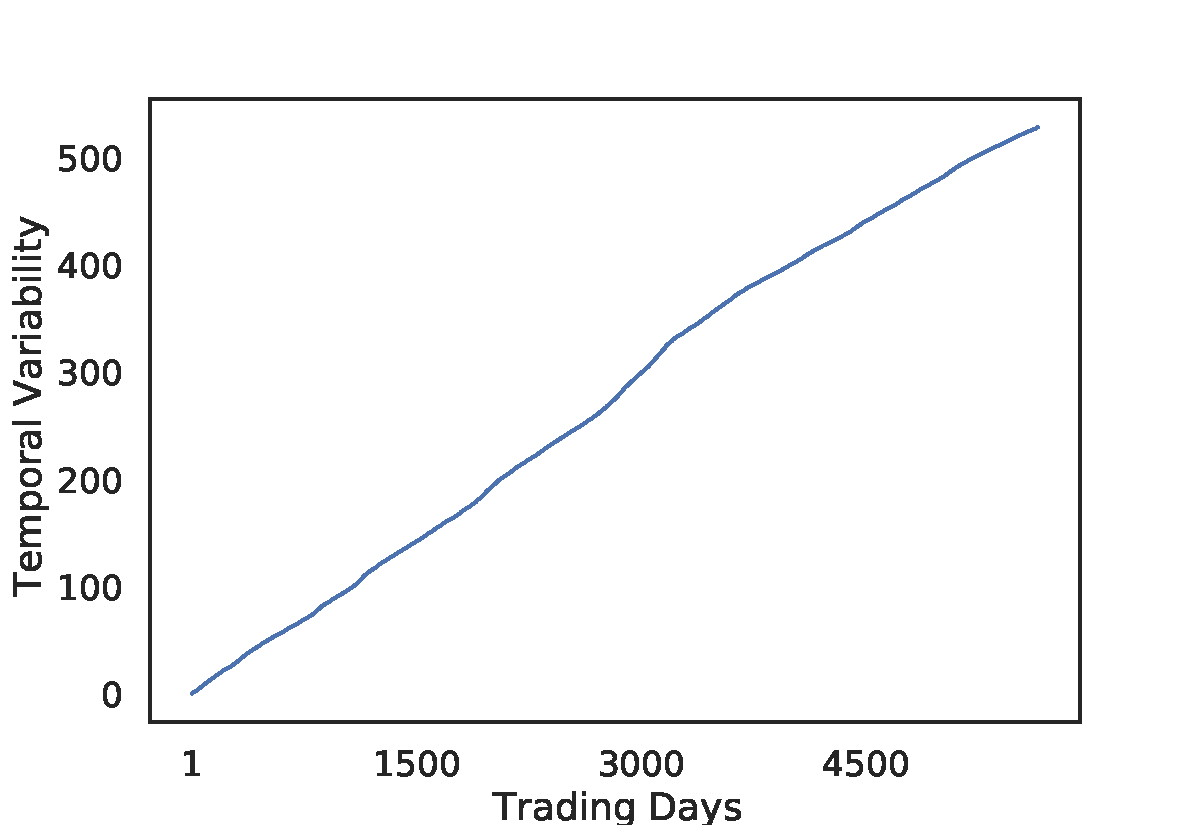
\includegraphics[width=4.5cm, keepaspectratio]{variation-functional_nyse-o} }}%
%    \,
%    \subfloat[NYSE (N)]{{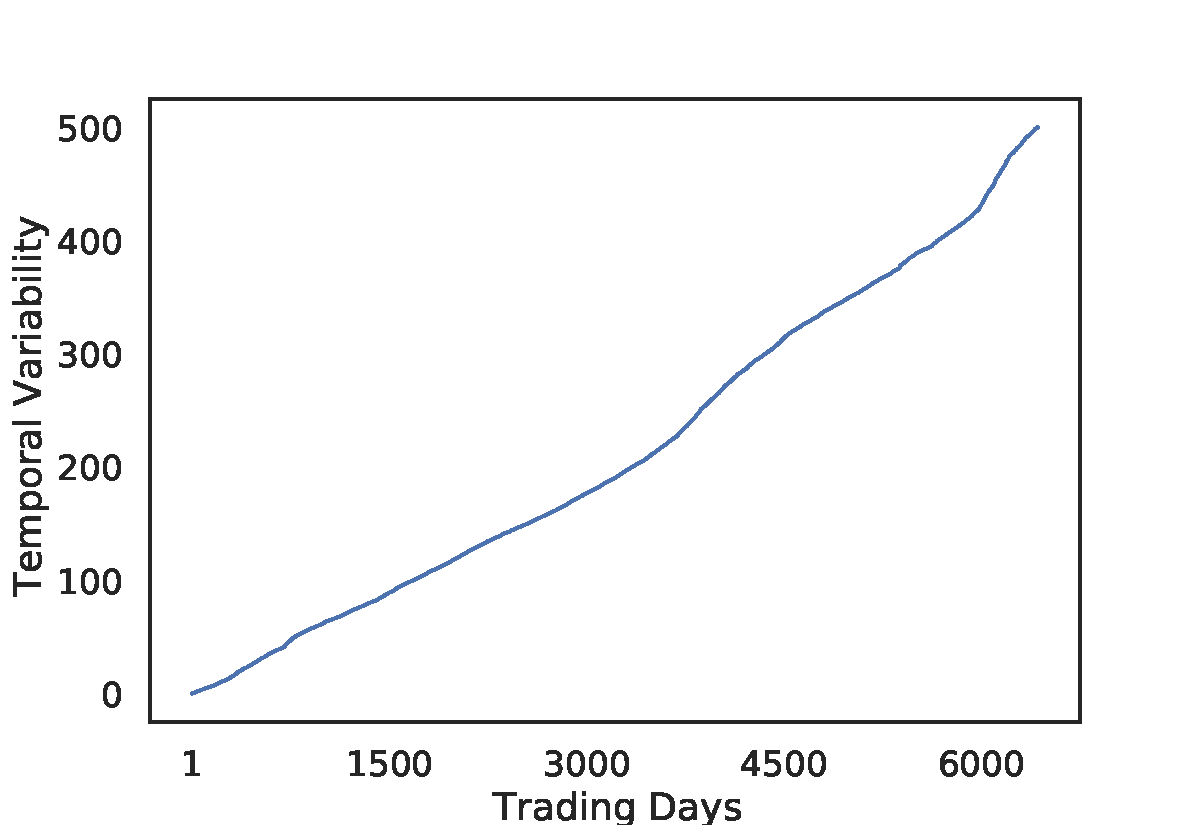
\includegraphics[width=4.5cm, keepaspectratio]{variation-functional_nyse-n} }}%
%    \,
%    \subfloat[TSE]{{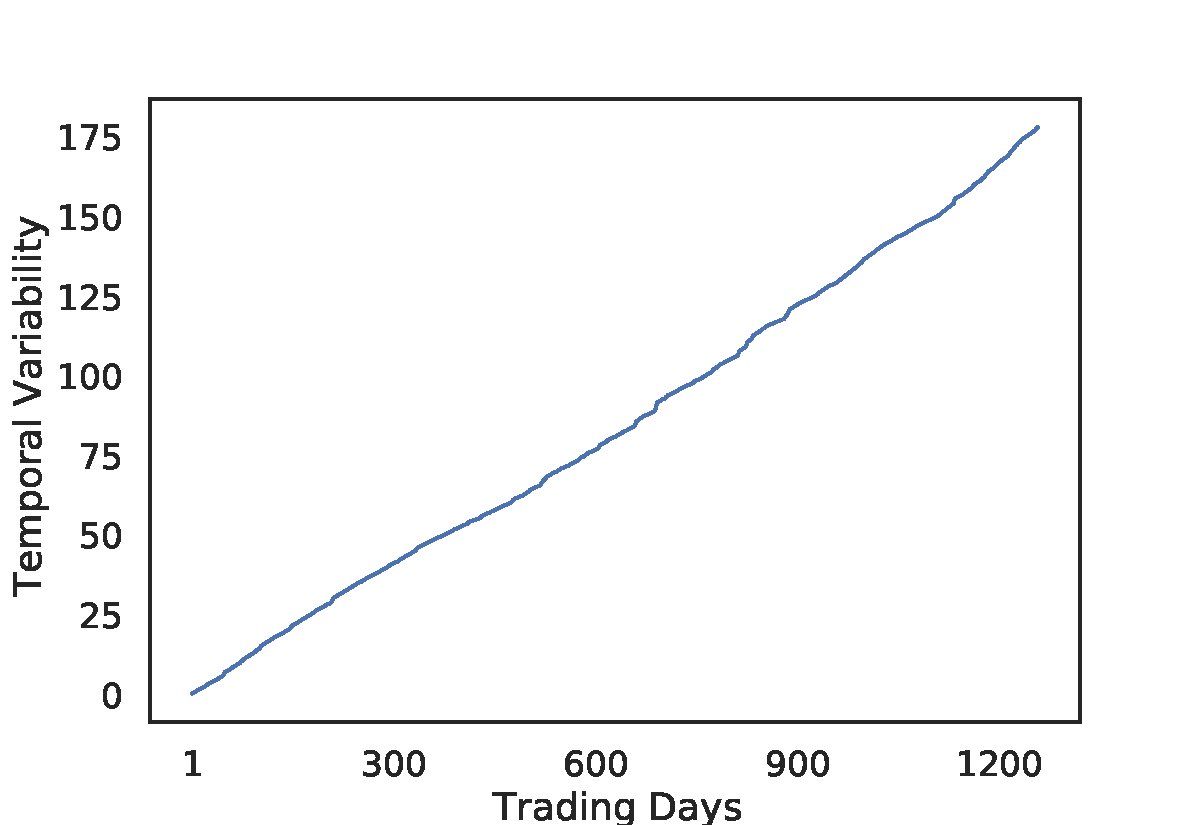
\includegraphics[width=4.5cm, keepaspectratio]{variation-functional_tse} }}%
%    
%    \subfloat[SP500]{{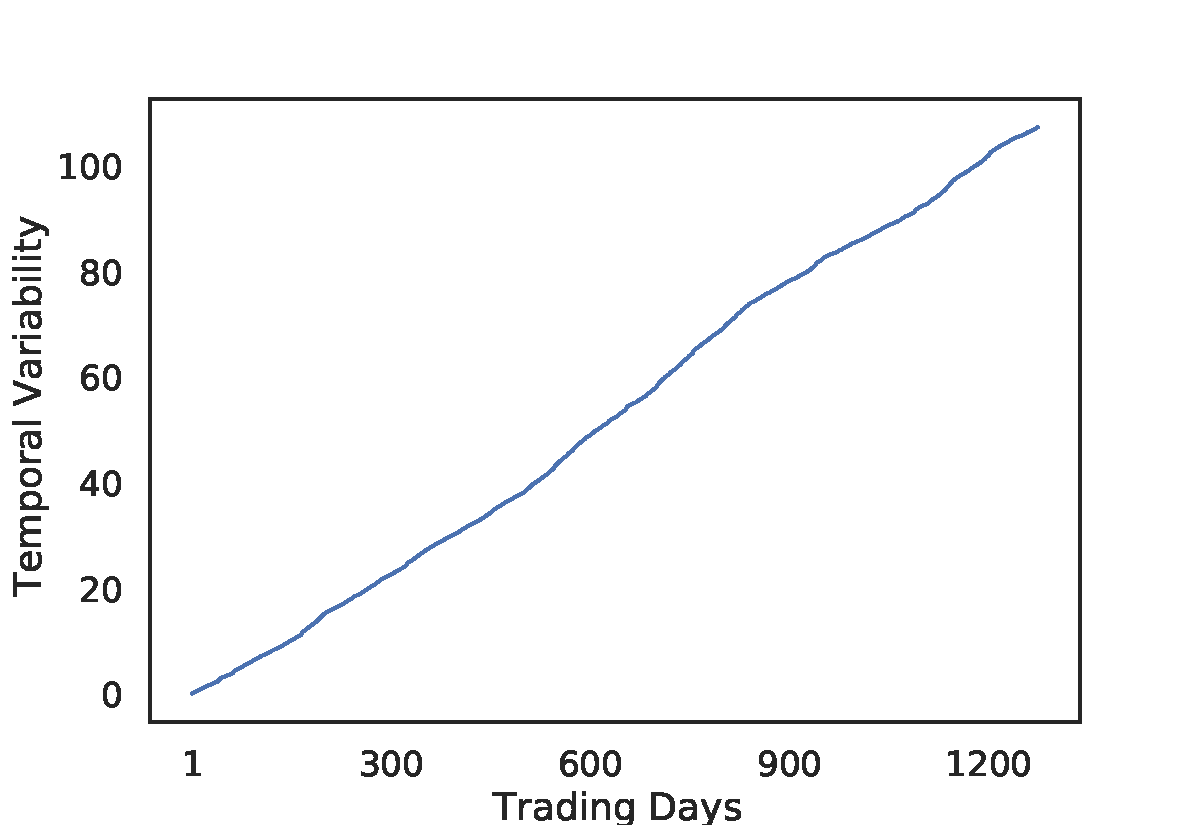
\includegraphics[width=4.5cm, keepaspectratio]{variation-functional_sp500} }}%
%    \,
%    \subfloat[MSCI]{{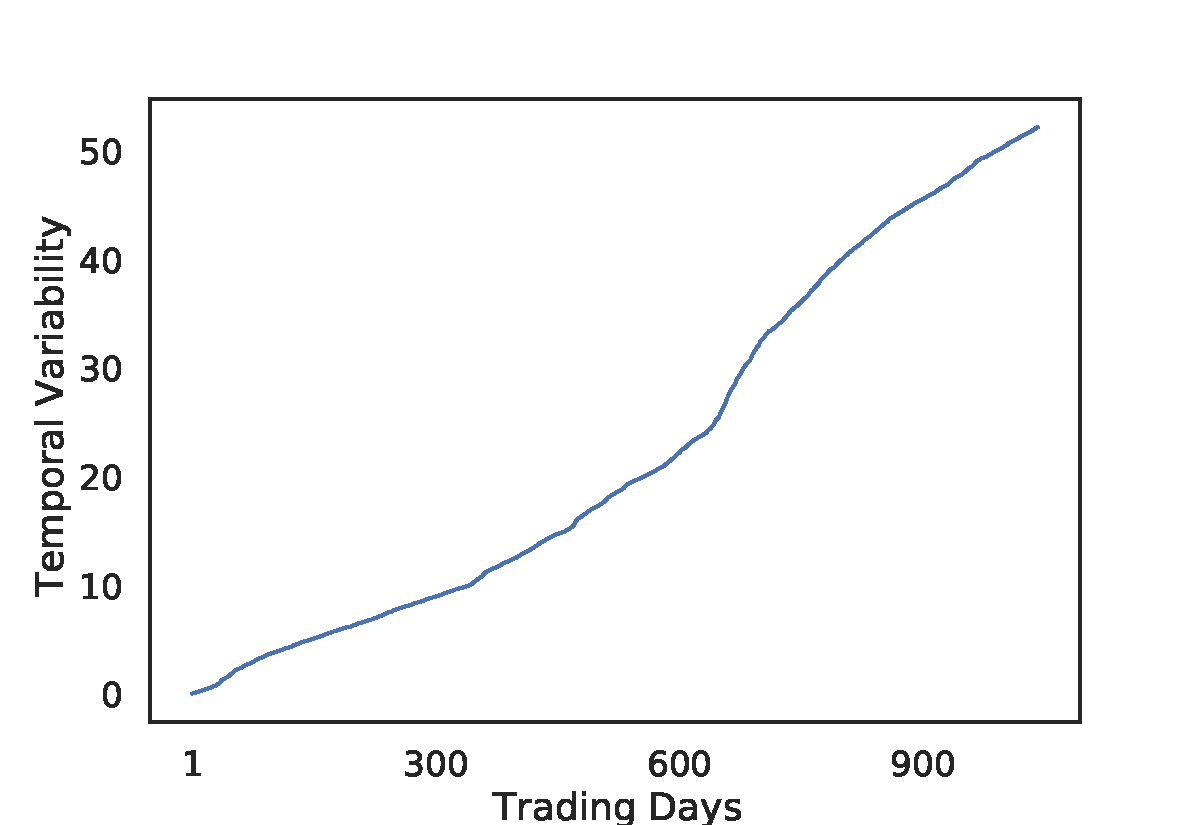
\includegraphics[width=4.5cm, keepaspectratio]{variation-functional_msci} }}%
%    \,
%    \subfloat[DJIA]{{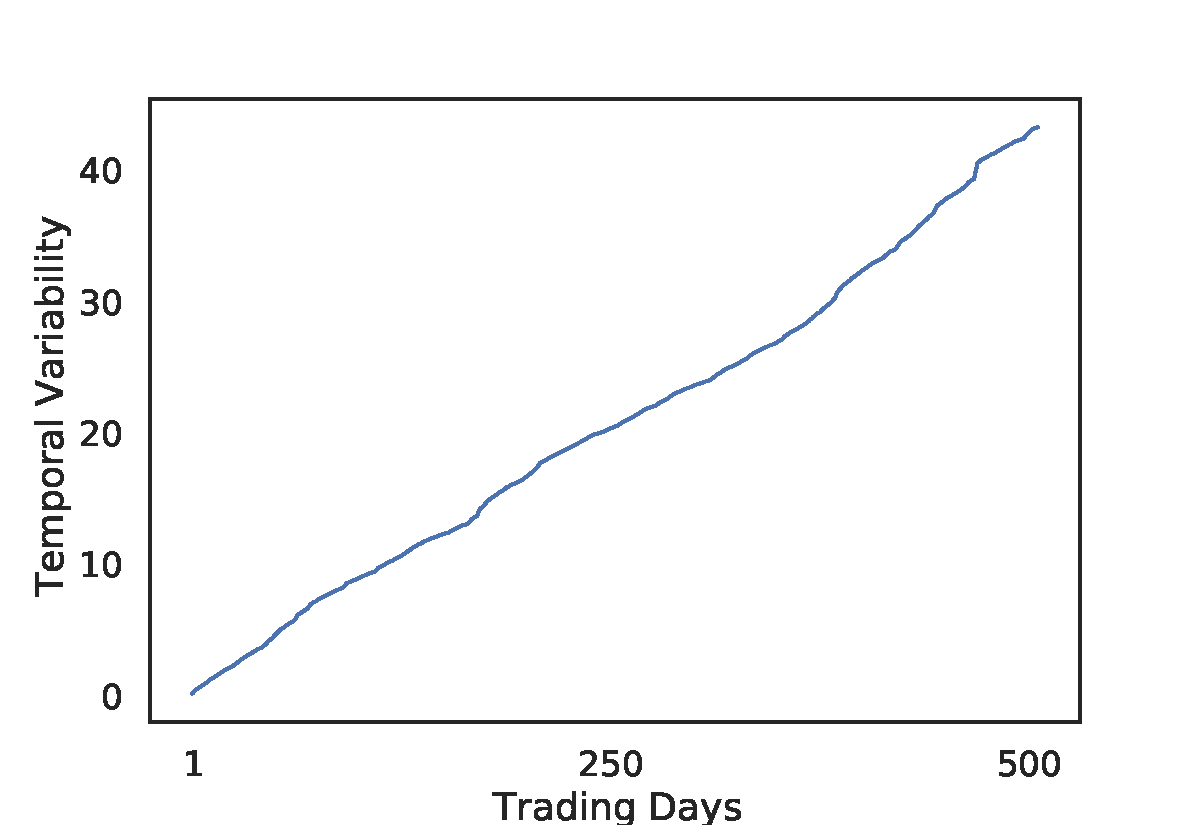
\includegraphics[width=4.5cm, keepaspectratio]{variation-functional_djia} }}%
%\end{figure}
\begin{mccorrection}
\begin{figure}[H]
\caption{Temporal variability $\mathrm{Var}(f_{1:T}) = \sum_{t=2}^T \Vert f_t - f_{t-1} \Vert_\infty$ for the six equity data sets from Table~\ref{tab:stock-datasets}. The solid red line represents the identity line (i.e. $y=x$).}
\label{fig:temporal-variation}
    \subfloat[NYSE (O)]{{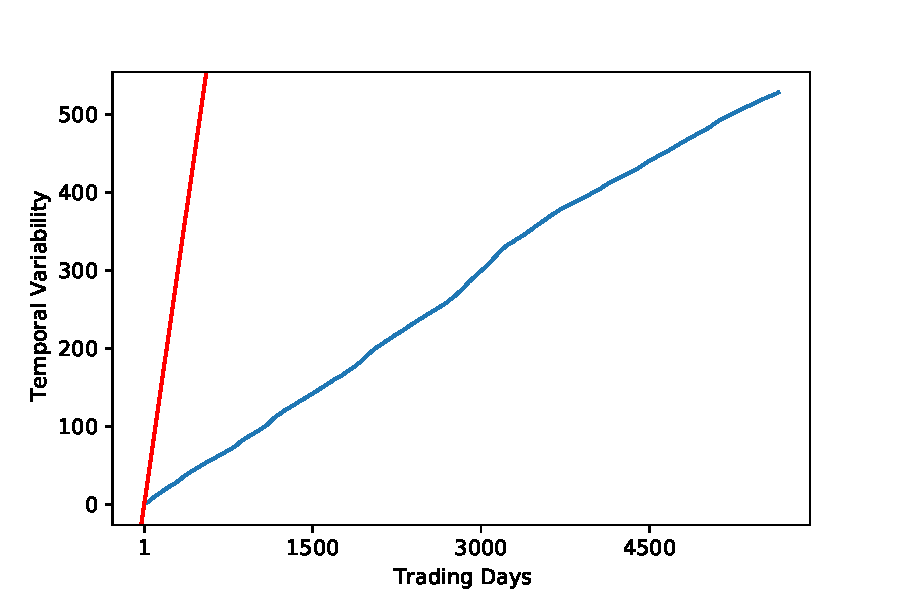
\includegraphics[width=4.5cm, keepaspectratio]{variation-functional_nyse-o_NEW} }}%
    \,
    \subfloat[NYSE (N)]{{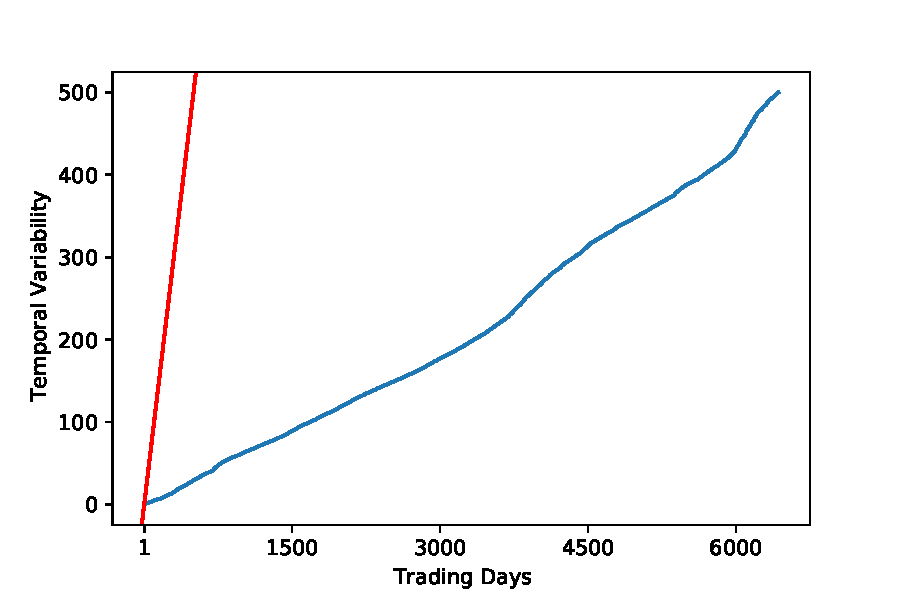
\includegraphics[width=4.5cm, keepaspectratio]{variation-functional_nyse-n_NEW} }}%
    \,
    \subfloat[TSE]{{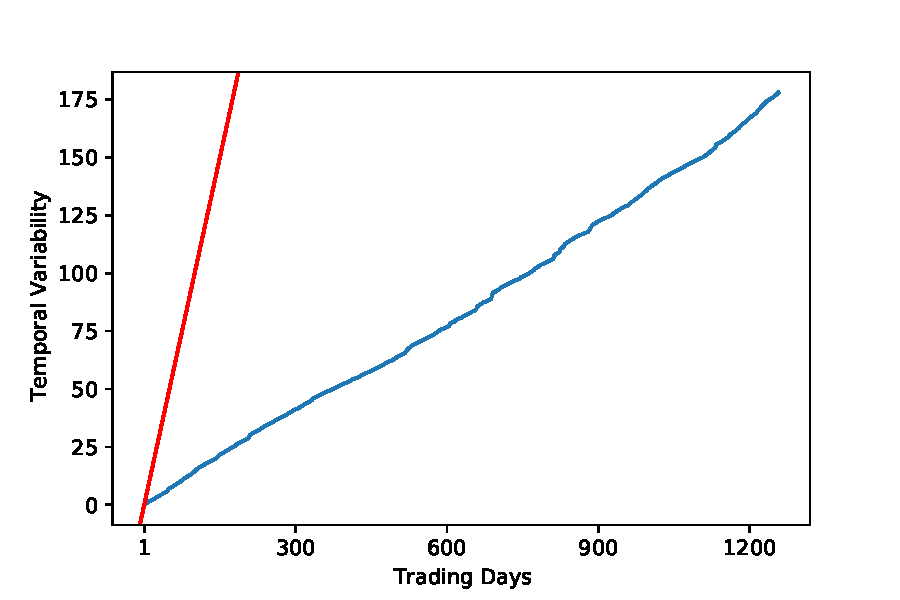
\includegraphics[width=4.5cm, keepaspectratio]{variation-functional_tse_NEW} }}%
    
    \subfloat[SP500]{{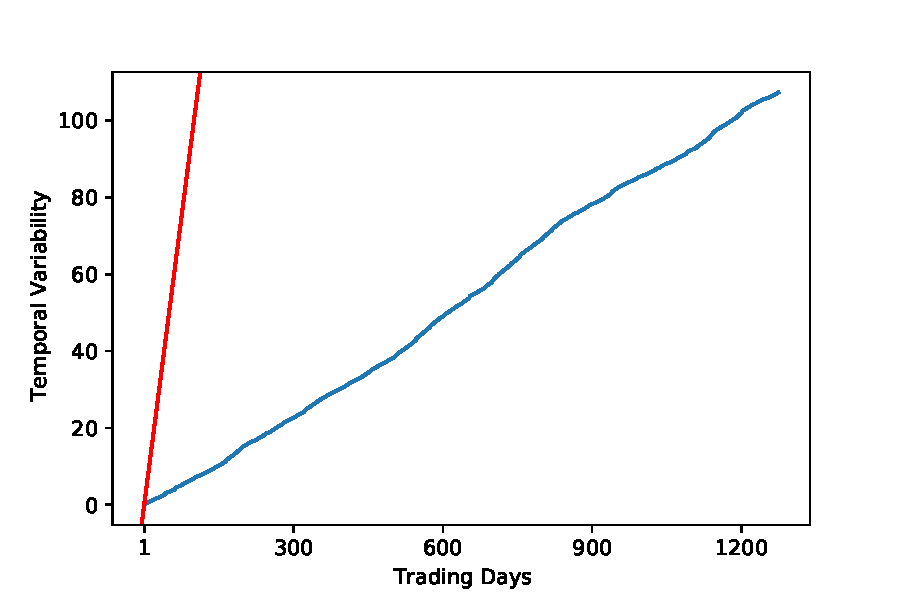
\includegraphics[width=4.5cm, keepaspectratio]{variation-functional_sp500_NEW} }}%
    \,
    \subfloat[MSCI]{{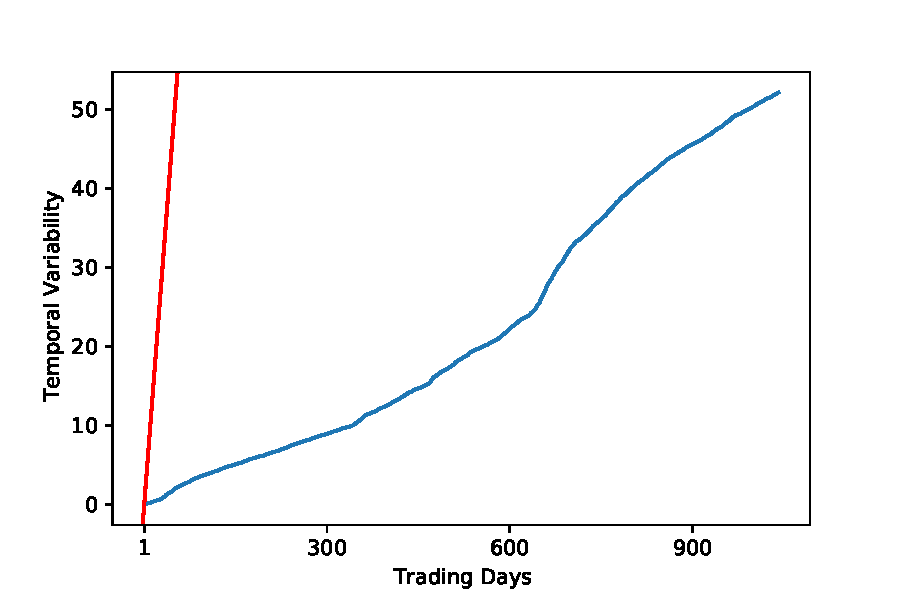
\includegraphics[width=4.5cm, keepaspectratio]{variation-functional_msci_NEW} }}%
    \,
    \subfloat[DJIA]{{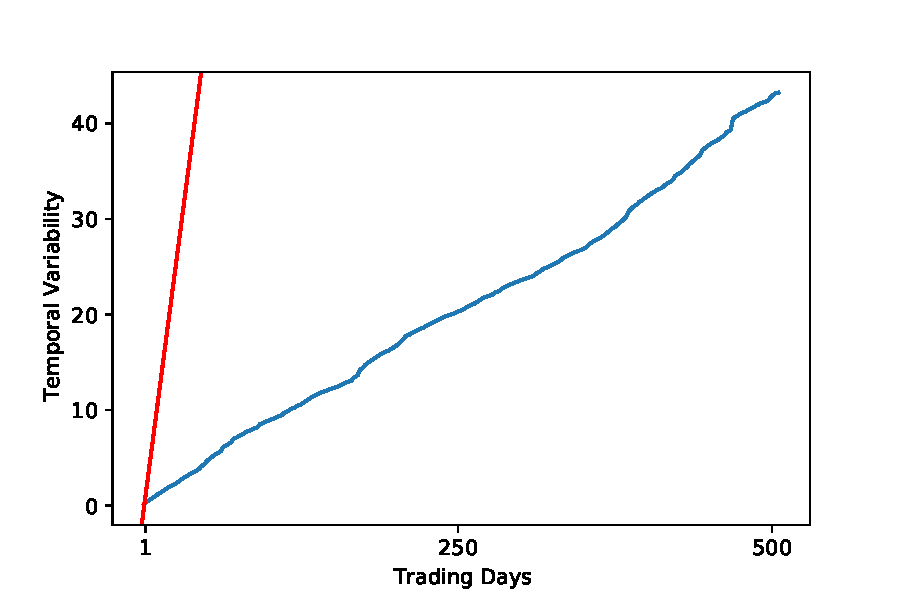
\includegraphics[width=4.5cm, keepaspectratio]{variation-functional_djia_NEW} }}%
\end{figure}
\end{mccorrection}
Figure~\ref{fig:variation-functional-boxplot} allows us to get a sense of the tracking-error magnitudes for the six equity data sets. Given the tight interquartile ranges and relatively low medians, we should not expect these to be very significant.
\begin{figure}[H]
\caption{Box plot of temporal-variability components $\Vert f_t - f_{t-1} \Vert_\infty$ across the six equity data sets presented in Table~\ref{tab:stock-datasets}.}
\label{fig:variation-functional-boxplot}
\begin{center}
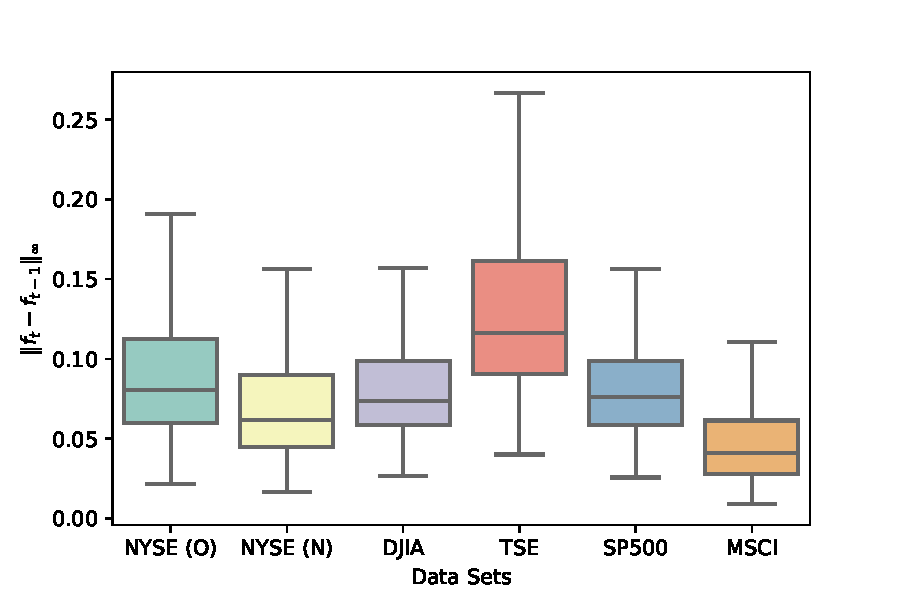
\includegraphics[width=\textwidth,height=\textheight,keepaspectratio]{variation-functional-boxplot}
\end{center}
\end{figure}

\subsection{Formulations}

\subsubsection{Single-period mean reversion}

Our single-period mean reversion algorithm, termed SingleOLMAX, is based on the single-period mean reversion ideas described in \citep[Section~4.1]{pamr}. The goal is to solve the problem in Eq. \eqref{eq:olps-problem}, with $f_t(\mathbf{b}) = \mathbf{b}^\text{T}\mathbf{x}_t$ instead of Eq. \eqref{eq:olps-loss-function}. The reason for this is because we seek to capitalise on the appreciation of poor-performing stocks, expecting their bad performance to be transient and to ultimately `revert to the mean', which calls for a \emph{follow-the-loser} investing approach.

We saw in the previous subsection that the temporal variability of the loss-function sequence is sublinear in $T$, for all the stock data sets. As shown in Proposition~\ref{prop:action-choices-dynamic-regret}, the following portfolio strategy will therefore achieve a sublinear tracking error:
\begin{equation}
\label{eq:single-olmax-criterion}
	\mathbf{b}_{t+1} \in \argmin_{\mathbf{b}\in\Delta_m}\; \mathbf{b}^\text{T}\mathbf{x}_t, \qquad t \in [T-1],
\end{equation}
with the convention that $\mathbf{b}_1 = \mathbf{1} / m$. To solve this linear program, it is convenient to first sort the components of $\mathbf{x}_t$ in ascending order, so that
\begin{equation}
	x_{t,1} \leq x_{t,2} \leq \ldots \leq x_{t,i} \leq \ldots \leq x_{t,m}.
\end{equation}
We then check the sign of $x_{t,1}$. If the latter is non-negative, then the minimal value of $\mathbf{b}^\text{T}\mathbf{x}_t$ is achieved by setting $b_{t+1,i} = 0$ for all $i\in[m]$, which, after performing the projection onto $\Delta_m$, results in the equally-weighted portfolio $\mathbf{1} / m$. Conversely, if $x_{t,1} < 0$, then the optimal weights are such that $b_{t+1,1} = 1$ and $b_{t+1,k} = 0$ for all $k > 1$. Wrapping up the two cases, we obtain the following strategy:
\begin{equation}
	b_{t+1,i} =
	\begin{cases}
		0 & \text{if } x_{t,1} \geq 0 \\
		\delta_{i1} & \text{otherwise}
	\end{cases},
	\qquad \forall\,t \in [T-1],\, \forall\,i \in [m],
\end{equation}
where $\delta_{ij}$ denotes the Kronecker delta. This choice is quite obvious: we allocate our entire budget to the investment with the lowest price relative.

The procedure is outlined in Algorithm~\ref{alg:single-period-olmax}. Note that it is completely hyperparameter-free and thereby not prone to the data-snooping bias, unlike its cousin PAMR.
\begin{algorithm}
  \caption{SingleOLMAX: Single-Period Online Maximum Reversion}
\label{alg:single-period-olmax}
  \begin{algorithmic}[1]
%    \STATE {\bfseries Input:} market sequence $\mathbf{x}_{1:T}$
    \STATE {\bfseries Initialisation:} initial portfolio $\mathbf{b}_1 = \frac{\mathbf{1}}{m}$, initial wealth $S_0 = 1$
    \FOR{$t=1, 2, \ldots, T$}
      \STATE observe stock price relatives $\mathbf{x}_t$
      \STATE update wealth:
        $
          S_t = S_{t-1} \times (\mathbf{b}_t^\text{T}\mathbf{x}_t)
        $
      \IF {$t < T$} 
        \STATE sort $\mathbf{x}_t$ in ascending order 
      \STATE update the portfolio:
	\begin{equation*}
		b_{t+1,i} =
		\begin{cases}
			0 & \text{if } x_{t,1} \geq 0 \\
			\delta_{i1} & \text{otherwise}
		\end{cases},
		\qquad i \in [m]
	\end{equation*}
	\ENDIF
    \ENDFOR
%    \STATE {\bfseries Output:} terminal wealth $S_T$
  \end{algorithmic}
\end{algorithm}

\subsubsection{Multiperiod mean reversion}

One common criticism of the single-period mean reversion assumption is that it fails to account for price reversals that occur over longer periods (see, e.g., \citep{olmar}). To overcome this limitation, we follow \citet{olmar}, and modify the SingleOLMAX criterion in Eq. \eqref{eq:single-olmax-criterion} as follows:  
\begin{equation}
\label{eq:multi-olmax-criterion}
	\mathbf{b}_{t+1} \in \argmax_{\mathbf{b}\in\Delta_m}\; \mathbf{b} \cdot \widetilde{\mathbf{x}}_{t+1}, \qquad t \in [T-1],
\end{equation}
where $\widetilde{\mathbf{x}}_{t+1}$ is a forecast of the $(t+1)$-th price-relative vector based upon the sequence $\mathbf{x}_{1:t}$ of observed price relatives. From a dynamic OCO standpoint, we can heuristically justify Eq. \eqref{eq:multi-olmax-criterion} via
\begin{equation}
	\argmax_{\mathbf{b}\in\Delta_m}\; \mathbf{b} \cdot \widetilde{\mathbf{x}}_{t+1}
	\approx \mathbf{b}_{t+1}^*,
\end{equation}
where $\mathbf{b}_{t+1}^*$ is the clairvoyant's optimal portfolio for period $(t+1)$, i.e.\ $\mathbf{b}_{t+1}^* = \argmax_{\mathbf{b}\in\Delta_m}\, \mathbf{b} \cdot \mathbf{x}_{t+1}$. By analogy with Eq. \eqref{eq:single-olmax-criterion}, after sorting $\widetilde{\mathbf{x}}_{t+1}$ in ascending order, we can write the unique solution to the optimisation problem in Eq. \eqref{eq:multi-olmax-criterion} as
\begin{equation}
	b_{t+1,i} =
	\begin{cases}
		0 & \text{if } \widetilde{x}_{t+1,m} \leq 0 \\
		\delta_{im} & \text{otherwise}
	\end{cases},
	\qquad \forall\,t \in [T-1],\, \forall\,i \in [m].
\end{equation}

We now discuss how to form the predictions $\widetilde{\mathbf{x}}_{t+1}$. The basic idea is to exploit the reversion of the current prices $\mathbf{p}_t$ to $\widetilde{\mathbf{p}}_{t+1} = \mathrm{MA}_t$, where $\mathrm{MA}_t$ denotes the moving average of price vectors at the end of period $t$. Following \citet{olmar}, we shall consider two types of moving average, namely a simple moving average (SMA)
\begin{equation}
\label{eq:sma}
	\mathrm{SMA}_t
	= \frac{1}{w}\sum_{\tau=t-w+1}^t \mathbf{p}_\tau,
\end{equation}
where $w$ denotes the size of the lookback window, and an exponential moving average (EMA)
\begin{equation}
\label{eq:ema}
	\mathrm{EMA}_t
	= \alpha\mathbf{p}_t + (1-\alpha)\mathrm{EMA}_{t-1},
\end{equation}
where $\alpha \in (0, 1)$ is the smoothing factor. The corresponding price-relative forecasts are respectively:
\begin{align}
	& \widetilde{\mathbf{x}}_{t+1}^\text{SMA}
	\equiv \frac{\mathrm{SMA}_t}{\mathbf{p}_t}
	= \frac{1}{w}\left(\frac{\mathbf{p}_t}{\mathbf{p}_t} + \frac{\mathbf{p}_{t-1}}{\mathbf{p}_t} + \ldots + \frac{\mathbf{p}_{t-w+1}}{\mathbf{p}_t}\right)
	= \frac{1}{w}\left(\mathbf{1} + \frac{1}{\mathbf{x}_t} + \ldots + \frac{1}{\bigotimes_{h=0}^{w-2}\mathbf{x}_{t-h}}\right),
	\\
	& \widetilde{\mathbf{x}}_{t+1}^\text{EMA}
	\equiv \frac{\mathrm{EMA}_t}{\mathbf{p}_t}
	= \frac{\alpha\mathbf{p}_t + (1-\alpha)\mathrm{EMA}_{t-1}}{\mathbf{p}_t}
%	= \alpha + (1-\alpha)\frac{\mathrm{EMA}_{t-1}}{\mathbf{p}_{t-1}}\frac{\mathbf{p}_{t-1}}{\mathbf{p}_t}
	= \alpha + (1-\alpha)\frac{\widetilde{\mathbf{x}}_{t}^\text{EMA}}{\mathbf{x}_t}.
\end{align}

We present the resulting two variants of our proposed multiperiod online maximum reversion (MultiOLMAX) method in Algorithm~\ref{alg:multiperiod-olmax}. Compared to their OLMAR counterparts in \citep{olmar}, they rely on a single hyperparameter instead of two, namely the window size $w$ for the SMA variant and the smoothing factor $\alpha$ for the EMA variant\footnote{OLMAR additionally depends on a reversion threshold $\epsilon$.}.
\begin{algorithm}
  \caption{MultiOLMAX: Multiperiod Online Maximum Reversion}
\label{alg:multiperiod-olmax}
  \begin{algorithmic}[1]
    \STATE {\bfseries Input:} Window size $w \geq 2$ (SMA variant), smoothing factor $0 < \alpha < 1$ (EMA variant)
    \STATE {\bfseries Initialisation:} initial portfolio $\mathbf{b}_1 = \frac{\mathbf{1}}{m}$, initial wealth $S_0 = 1$
    \FOR{$t=1, 2, \ldots, T$}
      \STATE observe stock price relatives $\mathbf{x}_t$
      \STATE update wealth:
        $
          S_t = S_{t-1} \times (\mathbf{b}_t^\text{T}\mathbf{x}_t)
        $
      \IF {$t < T$}
      	\STATE predict next price-relative vector:
	\begin{equation*}
		\widetilde{\mathbf{x}}_{t+1} =
		\begin{cases}
			\frac{1}{w}\left(\mathbf{1} + \frac{1}{\mathbf{x}_t} + \ldots + \frac{1}{\bigotimes_{h=0}^{w-2}\mathbf{x}_{t-h}}\right) & \text{(SMA variant)} \\
			\alpha + (1-\alpha)\frac{\widetilde{\mathbf{x}}_{t}}{\mathbf{x}_t} & \text{(EMA variant)}
		\end{cases}
	\end{equation*}
        \STATE sort $\widetilde{\mathbf{x}}_{t+1}$ in ascending order 
      \STATE update the portfolio:
	\begin{equation*}
		b_{t+1,i} =
	\begin{cases}
		0 & \text{if } \widetilde{x}_{t+1,m} \leq 0 \\
		\delta_{im} & \text{otherwise}
	\end{cases},
	\qquad i \in [m].
	\end{equation*}
	\ENDIF
    \ENDFOR
%    \STATE {\bfseries Output:} terminal wealth $S_T$
  \end{algorithmic}
\end{algorithm}


\section{Experiments}
\label{sec:experiments}

In this section, we will present an extensive set of empirical studies, including our experimental test bed, protocols, comparison schemes, results and a detailed empirical analysis.

\subsection{Experimental test bed on real data}

To be able to compare the empirical performance of our OLMAX framework against that of other OLPS strategies, we focus on historical daily stock prices. Earlier studies have restricted their empirical analyses to equity data as they can be readily obtained from public domains such as Yahoo! Finance and Google Finance\footnote{Yahoo! Finance: \url{https://finance.yahoo.com/}; Google Finance: \url{https://www.google.com/finance}.}, which ensures experimental reproducibility. Summarised in Table~\ref{tab:stock-datasets}, we employ six real and diverse data sets from several financial markets\footnote{The data sets from \citep{borodin04} --- NYSE (O), TSE, SP500 and DJIA --- can be found at \url{http://www.cs.technion.ac.il/~rani/portfolios/}. As for the remaining data sets and their respective composition, they can be downloaded from \url{http://www.cais.ntu.edu.sg/~chhoi/olps}.}.

The first data set, NYSE (O), is a standard data set pioneered by \citet{cover} and used in subsequent works \citep{eg, borodin04, ons, bnn}. This data set contains 5,651 daily price relatives of 36 stocks\footnote{According to \citet{eg}, the data set was originally collected by Hal Stern. The stocks are mainly those of large-cap companies listed on NYSE. However, we ignore the criteria that were used in selecting them.} from the New York Stock Exchange (NYSE) over a 22-year period from July 3, 1962 until December 31, 1984.

The second data set, NYSE (N), is an extended version of NYSE (O) collected by \citet{cwmr}. It covers the period from January 1, 1985 to June 30, 2010, i.e.\ a total of 6,431 trading days\footnote{The data before 2007 were collected by G\'{a}bor Gelencs\'{e}r \url{http://www.cs.bme.hu/~oti/portfolio/}, whereas \citet{cwmr} collected the remaining data from Yahoo! Finance.}. Note that it is limited to 23 rather than 36 stocks owing to mergers and bankruptcies.

The third and fourth data sets, TSE and SP500, were collected by \citet{borodin04}. The former consists of 88 stocks listed on the Toronto Stock Exchange (TSE) and contains price relatives over a period of 1,259 trading days, ranging from January 4, 1994 through December 31, 1998. As for SP500, it consists of the 25 stocks in the S\&P500 index with the largest market capitalisations. It ranges from January 2, 1998 to January 31, 2003 (1,276 trading days).

The fifth dataset is MSCI, which is a collection of global equity indices that constitute the MSCI World Index\footnote{The constituents of this index are available at MSCI Barra (https://www.msci.com/).}. It is made of 24 indices that represent the equity markets of 24 countries around the world and spans of a total of 1,043 trading days, ranging from April 1, 2006 to March 31, 2010. The final dataset is the DJIA dataset \citep{borodin04}, consisting of the 30 components of the Dow Jones Industrial Average index. DJIA contains 507 trading days, ranging from January 14, 2001 to January 14, 2003.

The above test bed enables us to examine the behaviour of the proposed strategies under different market circumstances. For example, it covers several well-known crises in equity markets, such as the dot-com bubble from 1995 to 2000 and the subprime mortgage crisis from 2007 to 2009. The main purpose of the five stock data sets is to test the capabilities of the proposed algorithms on regional stock markets, while the MSCI index data set aims to assess their empirical performance on global indices.

\subsection{Experimental setup and metrics}

Our experimental setup is as follows. For MultiOLMAX (Algorithm~\ref{alg:multiperiod-olmax}), we denote by MultiOLMAX-S and MultiOLMAX-E the variants with SMA and EMA forecasts, respectively. To make our results comparable to those of \citet{olmar}, we adopt their hyperparameter configuration, namely $w = 5$ and $\alpha = 0.3$, across all six equity data sets. We shall assess the sensitivity of OLMAX to hyperparameter selection in Section~\ref{sec:olmax-hyperparameter-sensitivity}.

Following the standard practice in the OLPS literature, we primarily compare different strategies in terms of terminal wealth and annualised Sharpe ratio \citep{sharpe}. In general, higher values of these metrics indicate better algorithms. To analyse a strategy's downside risk, we use the maximum drawdown (MDD) metric; the lower the MDD values, the less pronounced the strategy's downside. For convenience, we report all these metrics in Table~\ref{tab:metrics}.
\begin{table}[t]
  \caption{Summary of the performance metrics used in the evaluations.}
  \label{tab:metrics}
  \centering
  \resizebox{\textwidth}{!}{\begin{tabular}{lc}
    \toprule
    Critetion & Performance metrics \\
    \midrule
    Absolute return & Terminal wealth ($S_T$), Annual percentage yield (APY) \\
    Risk & Annualised standard deviation, Maximum drawdown (MDD) \\
    Risk-adjusted return & Annualised Sharpe ratio (SR) \\
    \bottomrule
  \end{tabular}}
\end{table}

\begin{mccorrection}
There is somewhat of a disconnect of the metrics used for benchmarking and the notion of regret, in the sense that while the performance metrics from Table~\ref{tab:metrics} are meaningful, the algorithms proposed in this thesis were devised in the spirit of regret. However, we refrained from measuring performance relative to regret as well because most of the OLPS techniques used for benchmarking purposes in this chapter do not optimise regret, but rather obey alternative optimisation criteria. Therefore, while we could have computed the regret of these OLPS methods and compare it against the regret of our proposed methods, we thought it would have been unfair towards these methods.
\end{mccorrection}

In the next subsection, we discuss one important practical issue in online portfolio selection, namely transaction costs. We defer the evaluation of the performance of OLMAX under transaction costs to Section~\ref{sec:transaction-costs}.

\subsection{Transaction costs}

While our model in Section~\ref{sec:olps-model} is concise and easy to understand, it omits the important and unavoidable issue of \emph{transaction costs}, which include commission fees and taxes imposed by brokers and governments, respectively\footnote{Besides these, other factors such as bid-ask spreads contribute to transaction costs.}.

Basically, there are two ways to handle the transaction-cost issue. The first is to omit transaction costs from the OLPS model in the first instance to then adopt the \emph{proportional transaction cost} model \citep{blum99}. The second is to directly integrate the costs into the model \citep{gyorfi08}. Since the former approach is the most common in the OLPS literature, we shall follow it here. Specifically, at the beginning of period $t$, the portfolio manager rebalances to a new portfolio $\mathbf{b}_t$ from the last close-price adjusted portfolio $\widehat{\mathbf{b}}_{t-1}$, each component of which is calculated as $\widehat{b̂}_{t-1,i} = \frac{b_{t-1,i} \times x_{t-1,i}}{\mathbf{b}_{t-1}^\text{T}\mathbf{x}_{t-1}}$. Letting $\gamma \in (0, 1)$ be the transaction-cost rate, this rebalancing step incurs a transaction cost of $\frac{\gamma}{2}\sum_{i=1}^m |b_{t,i} - \widehat{b̂}_{t-1,i}|$, with the initial portfolio being set to the zero vector. Thus, the wealth after $T$ periods can be expressed as
\begin{equation}
	S_T^\gamma
	= S_0 \prod_{t=1}^T \left[(\mathbf{b}_t^\text{T}\mathbf{x}_t) \times \left(1 - \frac{\gamma}{2}\sum_{i=1}^m |b_{t,i} - \widehat{b̂}_{t-1,i}|\right)\right].
\end{equation}

\subsection{Comparison approaches}
\label{sec:comparison-approaches}

We shall compare the proposed algorithms against a number of benchmarks and representative strategies enumerated below, all of which provide extensive empirical evaluations in their respective studies. All parameters are set to the same values used in the corresponding papers\footnote{We could tune these parameters to improve performance, but this is beyond the scope of this thesis.}. Because this chapter has an empirical focus, we omit algorithms that place an emphasis on theoretical analysis and lack thorough experimentation.
\begin{enumerate}
  \item Market: Market strategy, that is, the uniform buy-and-hold (BAH) strategy;
  \item Best stock: Stock with the best performance in hindsight throughout the $T$-period horizon;
%  \item CRP: Constant Rebalanced Portfolio strategy \citep{cover};
%  \item UCRP: Uniform Constant Rebalanced Portfolio strategy \citep{cover};
  \item BCRP: Best constant rebalanced portfolio strategy in hindsight \citep{cover};
  \item UP: Cover's universal portfolios, based on the implementation of \citet{kalai02}, in which the parameters are such that $\delta_0 = 0.004$, $\delta = 0.005$, $m = 100$ and $S = 500$;
  \item EG: Exponentiated gradient algorithm with the best learning rate $\eta = 0.05$, as suggested by \citet{eg};
  \item ONS: Online Newton step with the parameters suggested by \cite{ons}, i.e.\ $\eta = 0$, $\beta = 1$ and $\gamma = \frac{1}{8}$;
  \item Anticor: BAH$_{30}$(Anticor), i.e.\ uniform buy-and-hold investment on the algorithms Anticor$_w$ with $w = 2, 3, \ldots, 30$, which achieves the best performance among the three solutions proposed by \citet{borodin04};
  \item $\text{B}^\text{K}$: Non-parametric kernel-based moving window strategy with $W = 5$, $L = 10$ and threshold $c = 1.0$, which exhibits the best empirical performance according to \citet{bnn};
   \item $\text{B}^\text{NN}$: Non-parametric nearest-neighbour strategy with parameter values $W = 5$, $L = 10$ and $p_l = 0.02 + 0.5\frac{l-1}{L-1}$, as \citet{bnn2} suggested;
  \item CORN: Correlation-driven non-parametric learning approaches \citep{corn} with parameters $W = 5$, $P = 1$ and $\rho = 0.1$.
  \item PAMR: Passive-aggressive mean reversion \citep{pamr} with parameter $\epsilon=0.5$;
  \item CWMR: Confidence-weighted mean reversion \citep{cwmr} algorithm (exact version) with $\epsilon = 0.5$;
  \item OLMAR-S: Online moving average reversion \citep{olmar} with SMA price-relative forecasts, and parameters $\epsilon = 10$ and $w = 5$;
  \item OLMAR-E: Online moving average reversion \citep{olmar} with EMA price-relative forecasts, and parameters $\epsilon = 10$ and $\alpha = 0.3$.
%  \item RMR: Robust Median Reversion \citep{rmr} with parameters $W = 5$, $\epsilon = 10$ and $\tau = 0.001$;
%  \item OLPAPS: Online Passive-Aggressive Portfolio Selection (Algorithms~\ref{alg:olpaps-I} and~\ref{alg:olpaps-II}) with $\epsilon = 0.01$;
%  \item Kelly: \href{https://en.wikipedia.org/wiki/Kelly_criterion#Application_to_the_stock_market}{Kelly criterion};
\end{enumerate}
%The above list is also summarised in Table~\ref{olps-algos}.
%\begin{table}
%  \caption{OLPS algorithms evaluated and compared in our experiments.}
%  \label{olps-algos}
%  \centering
%  \resizebox{\textwidth}{!}{\begin{tabular}{lccc}
%    \toprule
%    Algorithm & Acronym & Type & Reference \\
%    \midrule
%    Buy and Hold & BAH & Benchmark & n/a \\
%    Constant Rebalanced Portfolio & CRP & Benchmark & \cite{cover} \\
%    Uniform CRP & UCRP & Benchmark & \cite{cover} \\
%    Best CRP & BCRP & Benchmark & \cite{cover} \\
%    Exponential Gradient & EG & Follow the Winner & \cite{eg} \\
%    Online Newton Step & ONS & Follow the Winner & \cite{ons} \\
%    Anticorrelation & Anticor & Follow the Loser & \cite{anticor} \\
%    Passive Aggressive Mean Reversion & PAMR & Follow the Loser & \cite{pamr} \\
%    Confidence Weighted Mean Reversion & CWMR & Follow the Loser & \cite{cwmr} \\
%    On-Line Moving Average Reversion & OLMAR & Follow the Loser & \cite{olmar} \\
%    Robust Median Reversion & RMR & Follow the Loser & \cite{rmr} \\
%    On-Line Passive-Aggressive Portfolio Selection & OLPAPS & Follow the Loser & this thesis \\
%    Kelly fractional betting & Kelly & Pattern Matching & \href{https://en.wikipedia.org/wiki/Kelly_criterion#Application_to_the_stock_market}{Kelly criterion} \\
%    Correlation-driven non-parametric learning & CORN & Pattern Matching & \cite{corn} \\
%    \bottomrule
%  \end{tabular}}
%\end{table}

\subsection{Experimental results -- terminal wealth}

Table~\ref{tab:terminal-wealth} reports the terminal wealth achieved by various approaches on the six equity data sets listed in Table~\ref{tab:stock-datasets}. From this perspective, the OLMAX algorithms are among the top two performers across five data sets (the exception being MSCI), and they achieve the best performance on four of them. On the well-known benchmark NYSE (O) data set, OLMAX significantly outperforms the state of the art, and likewise on the TSE and SP500 data sets. Although most existing algorithms other than Anticor and OLMAR-S perform badly on the DJIA data set, OLMAX achieves the highest final wealth, which further motivates the main idea behind the framework (see Section~\ref{sec:olmax-motivation}). Besides, the use of exponential rather than simple moving averages provides a significant performance boost on the NYSE (O) and NYSE (N) data sets.
\begin{table}[H]
  \caption{Terminal wealth achieved by various OLPS strategies on the six equity data sets from Table~\ref{tab:stock-datasets}. The top two results on each data set are highlighted in \textbf{bold}.}
  \label{tab:terminal-wealth}
  \centering
  \resizebox{\textwidth}{!}{\begin{tabular}{lcccccc}
    \toprule
    Methods & NYSE (O) & NYSE (N) & DJIA & TSE & SP500 & MSCI \\
    \midrule
	Market & 14.50 & 18.06 & 0.76 & 1.61 & 1.34 & 0.91 \\
	Best stock & 54.14 & 83.51 & 1.19 & 6.28 & 3.78 & 1.50 \\
	BCRP & 250.60 & 120.32 & 1.24 & 6.78 & 4.07 & 1.51 \\
%	UP & 26.99 & 31.07 & 0.81 & 1.59 & 1.64 & 0.92 \\
	\\
	UP & 26.68 & 31.49 & 0.81 & 1.60 & 1.62 & 0.92 \\
	EG & 27.09 & 31.00 & 0.81 & 1.59 & 1.63 & 0.93 \\
%	ONS & 109.28 & 21.43 & 1.53 & 1.62 & 3.34 & 0.86 \\
	ONS & 109.19 & 21.59 & 1.53 & 1.62 & 3.34 & 0.86 \\
	\\
	$\text{B}^\text{K}$ & 1.08E+09 & 4.64E+03 & 0.68 & 1.62 & 2.24 & 2.64 \\
	$\text{B}^\text{NN}$ & 3.35E+11 & 6.80E+04 & 0.88 & 2.27 & 3.07 & 13.47 \\
	CORN & 1.48E+13 & 5.37E+05 & 0.84 & 3.56 & 6.35 & \textbf{26.10} \\
	\\
	Anticor & 2.41E+08 & 6.21E+06 & \textbf{2.29} & 39.36 & 5.89 & 3.22 \\
	PAMR & 5.14E+15 & 1.25E+06 & 0.68 & 264.86 & 5.09 & 15.23 \\
%	CWMR & 5.55E+15 & 1.31E+06 & 0.68 & 193.86 & 4.98 & 14.93 \\
	CWMR & 6.49E+15 & 1.41E+06 & 0.68 & 332.62 & 5.90 & 17.28 \\
%	OLMAR & 7.88E+16 & 4.23E+08 & 2.26 & 58.59 & 16.37 & 14.72 \\
	\\
	OLMAR-S & 3.68E+16 & 2.54E+08 & 2.12 & 424.80 & 5.83 & 16.39 \\
	OLMAR-E & \textbf{1.09E+18} & \textbf{5.10E+08} & 1.20 & \textbf{678.44} & 8.63 & \textbf{21.21} \\
	\\
	SingleOLMAX & 4.09E+15 & 5.09E+05 & 0.59 & \textbf{1.56E+03} & 8.32 & 7.30 \\
	MultiOLMAX-S & 4.47E+16 & 3.86E+08 & \textbf{2.51} & 75.88 & \textbf{15.30} & 11.19 \\
	MultiOLMAX-E & \textbf{2.54E+18} & \textbf{4.80E+08} & 1.22 & 313.09 & \textbf{14.31} & 13.44 \\
%	\\
%	AdaPAMR & 1.08E+07 & 3.03E+05 & 0.69 & 216.69 & 6.90 & 15.06 \\
%	AdaOLMAR & 6.82E+04 & 774.05 & 2.16 & 25.33 & 5.86 & 4.10 \\
%	\\
%	MAPGRAD & 1.11E+08 & 1.79E+05 & 0.67 & 222.35 & 6.85 & 13.82 \\
    \bottomrule
  \end{tabular}}
\end{table}
In order to confirm that the above OLMAX results are not a statistical fluke, we compute the alphas and betas from the regression
\begin{equation}
	r_t^\text{OLMAX} - r_f
	= \alpha + \beta(r_t^\text{MKT} - r_f) + \varepsilon_t,
\end{equation}
where $r_t^\text{OLMAX}$ denotes the return of an OLMAX portfolio at time $t$, $r_f$ is the risk-free rate, and $r_t^\text{MKT}$ represents a passive exposure to the stock market, proxied by the return on the BAH strategy. Table~\ref{tab:stat-tests} displays the $t$-statistics and $p$-values of the estimated alphas for the MultiOLMAX-S variant. From this table, we see that the probability that the outstanding MultiOLMAX-S performance is due to luck is at most 1.31\%. Though we omitted them here, the findings are similar for other OLMAX variants. Thus, we can claim with almost absolute certainty that OLMAX outperforms the state of the art on the equity data sets.
\begin{table}[H]
  \caption{Statistical tests of the performance achieved by the MultiOLMAX-S algorithm on the stock data sets. The acronym MER stands for `mean excess return'.}
  \label{tab:stat-tests}
  \centering
  \resizebox{\textwidth}{!}{\begin{tabular}{lcccccc}
    \toprule
    Stat. Attr. & NYSE (O) & NYSE (N) & DJIA & TSE & SP500 & MSCI \\
    \midrule
	Size & 5651 & 6431 & 507 & 1259 & 1276 & 1043 \\   
	MER (MultiOLMAX-S) & 0.0073 & 0.0035 & 0.0022 & 0.0050 & 0.0026 & 0.0025 \\ 
%	MER (Market) & 0.0004 & 0.0004 & -0.0006 & 0.0003 & 0.0002 & -0.0001 \\
	MER (Market) & 0.0005 & 0.0005 & -0.0004 & 0.0004 & 0.0003 & 0.0000 \\
	Winning Ratio & 57.95\% & 55.19\% & 53.77\% & 55.15\% & 52.51\% & 55.88\% \\
	\\
	$\alpha$ & 0.0068 & 0.0031 & 0.0029 & 0.0046 & 0.0023 & 0.0026 \\   
	$\beta$ & 1.2709 & 1.1407 & 1.2540 & 1.6497 & 1.2541 & 1.1921 \\
	\\   
	$t$-stat & 15.1105 & 7.5234 & 2.4888 & 2.7452 & 2.9378 & 5.1207 \\   
	$p$-value & 0.0000 & 0.0000 & 0.0131 & 0.0061 & 0.0034 & 0.0000 \\  
    \bottomrule
  \end{tabular}}
\end{table}

\subsection{Experimental results -- risk-adjusted returns}

We now evaluate the volatility and maximum drawdown of different OLPS strategies, as well as their respective risk-adjusted returns as measured by the annualised Sharpe ratio \citep{sharpe}. Figure~\ref{fig:stock-metrics} displays these metrics for the six equity data sets. In addition to the proposed MultiOLMAX-S algorithm, we plot two benchmarks (Market and BCRP) and five state-of-the-art algorithms (Anticor, CORN, PAMR, CWMR and OLMAR\footnote{Henceforth, the acronym `OLMAR' will refer to the OLMAR-S strategy, i.e.\ the variant with SMA forecasts of price relatives.}).

In the previous paragraph, we saw that MultiOLMAX-S achieves the highest cumulative return on the majority of equity data sets. However, high return is typically associated with high risk. This is corroborated by Figures~\ref{fig:stock-metrics}(a) and (b), which show that the proposed method is one the riskiest in terms of volatility and maximum drawdown, respectively.

However, in spite of its high risk, MultiOLMAX-S yields a highly competitive Sharpe ratio, as illustrated by Figure~\ref{fig:stock-metrics}(c). This encouraging finding demonstrates that the proposed method is able to strike a good balance between risk and return, even though we do not explicitly account for risk in its formulation.

\begin{figure}[htp]
\caption{\footnotesize Risk and risk-adjusted performance of various OLPS strategies on the six stock data sets. In each diagram, the rightmost bar represents the result of our proposed strategy.}
\label{fig:stock-metrics}
\centering

\subfloat[Volatility Risk]{%
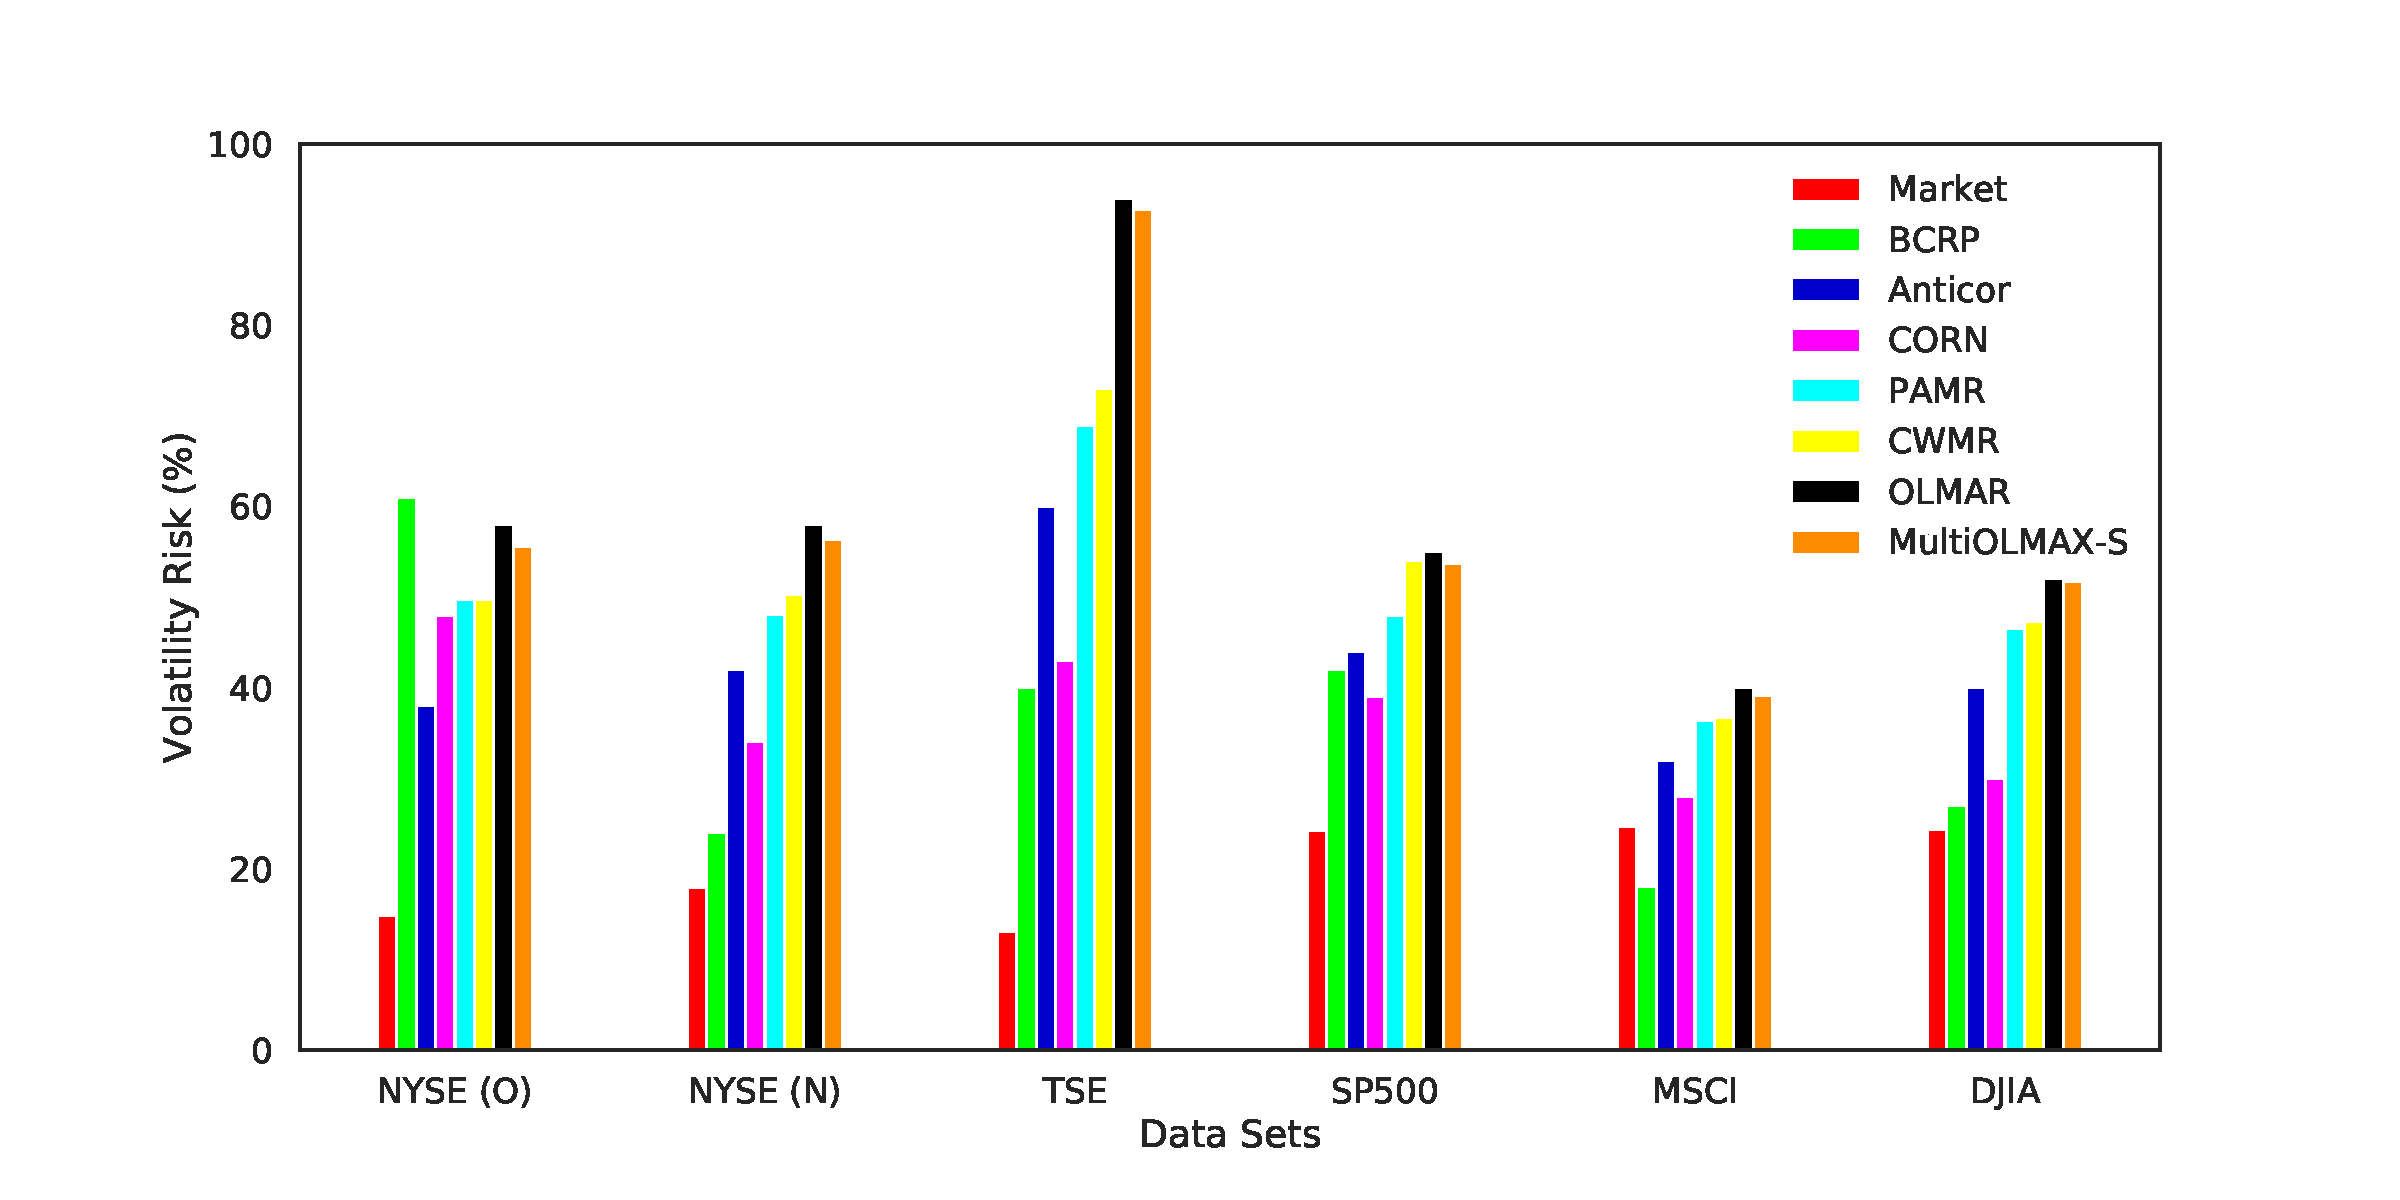
\includegraphics[width=\textwidth,height=\textheight,keepaspectratio]{vols}%
}

\subfloat[Drawdown Risk]{%
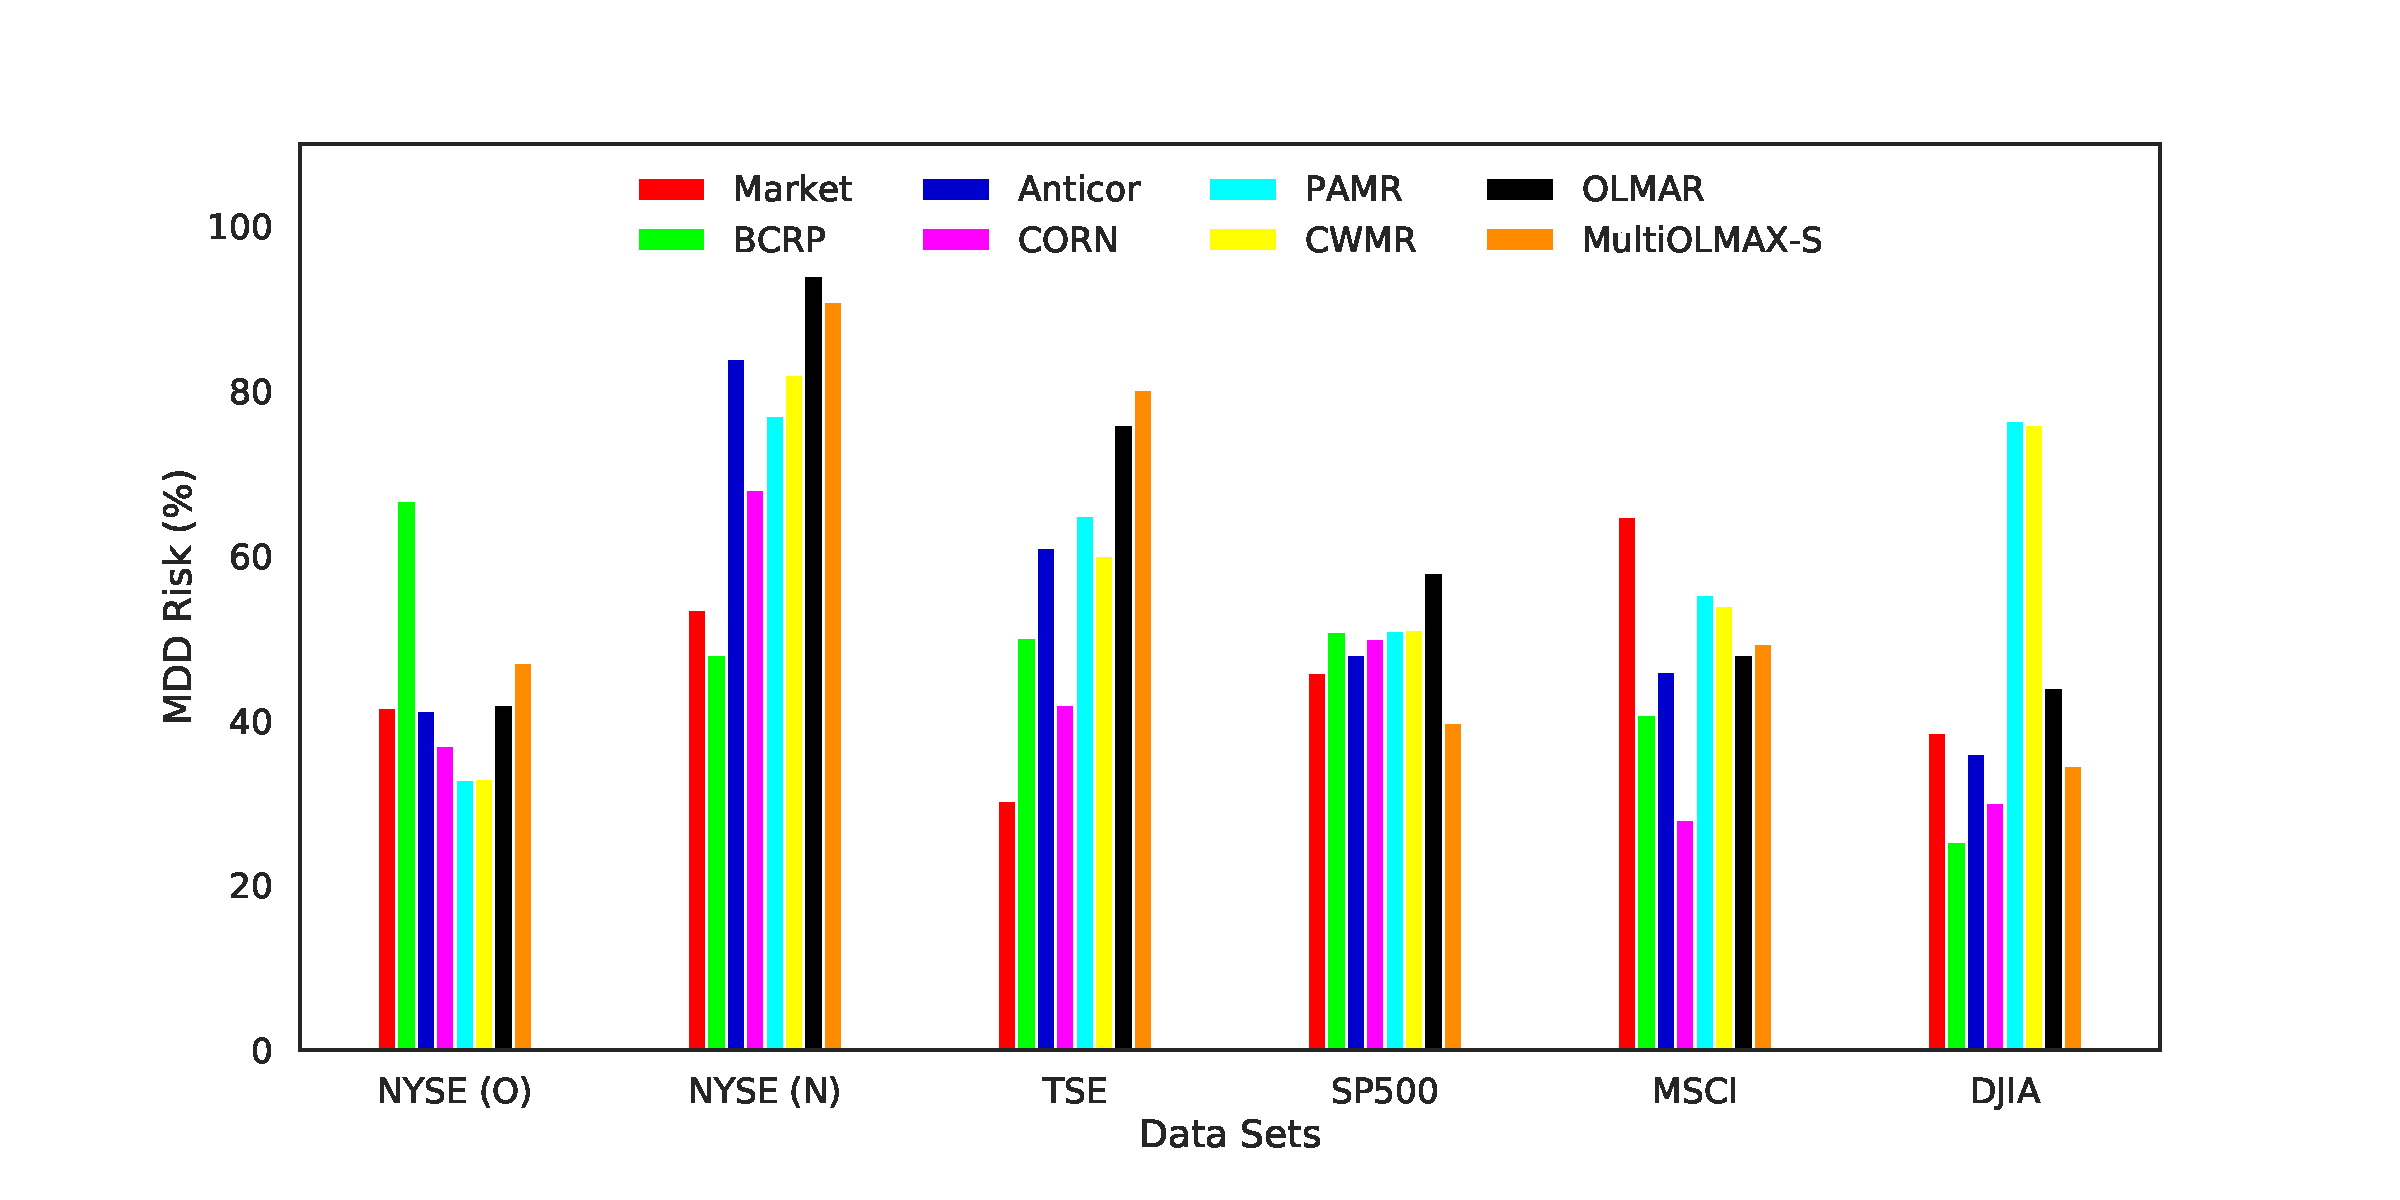
\includegraphics[width=\textwidth,height=\textheight,keepaspectratio]{mdds}%
}

\subfloat[Sharpe Ratio]{%
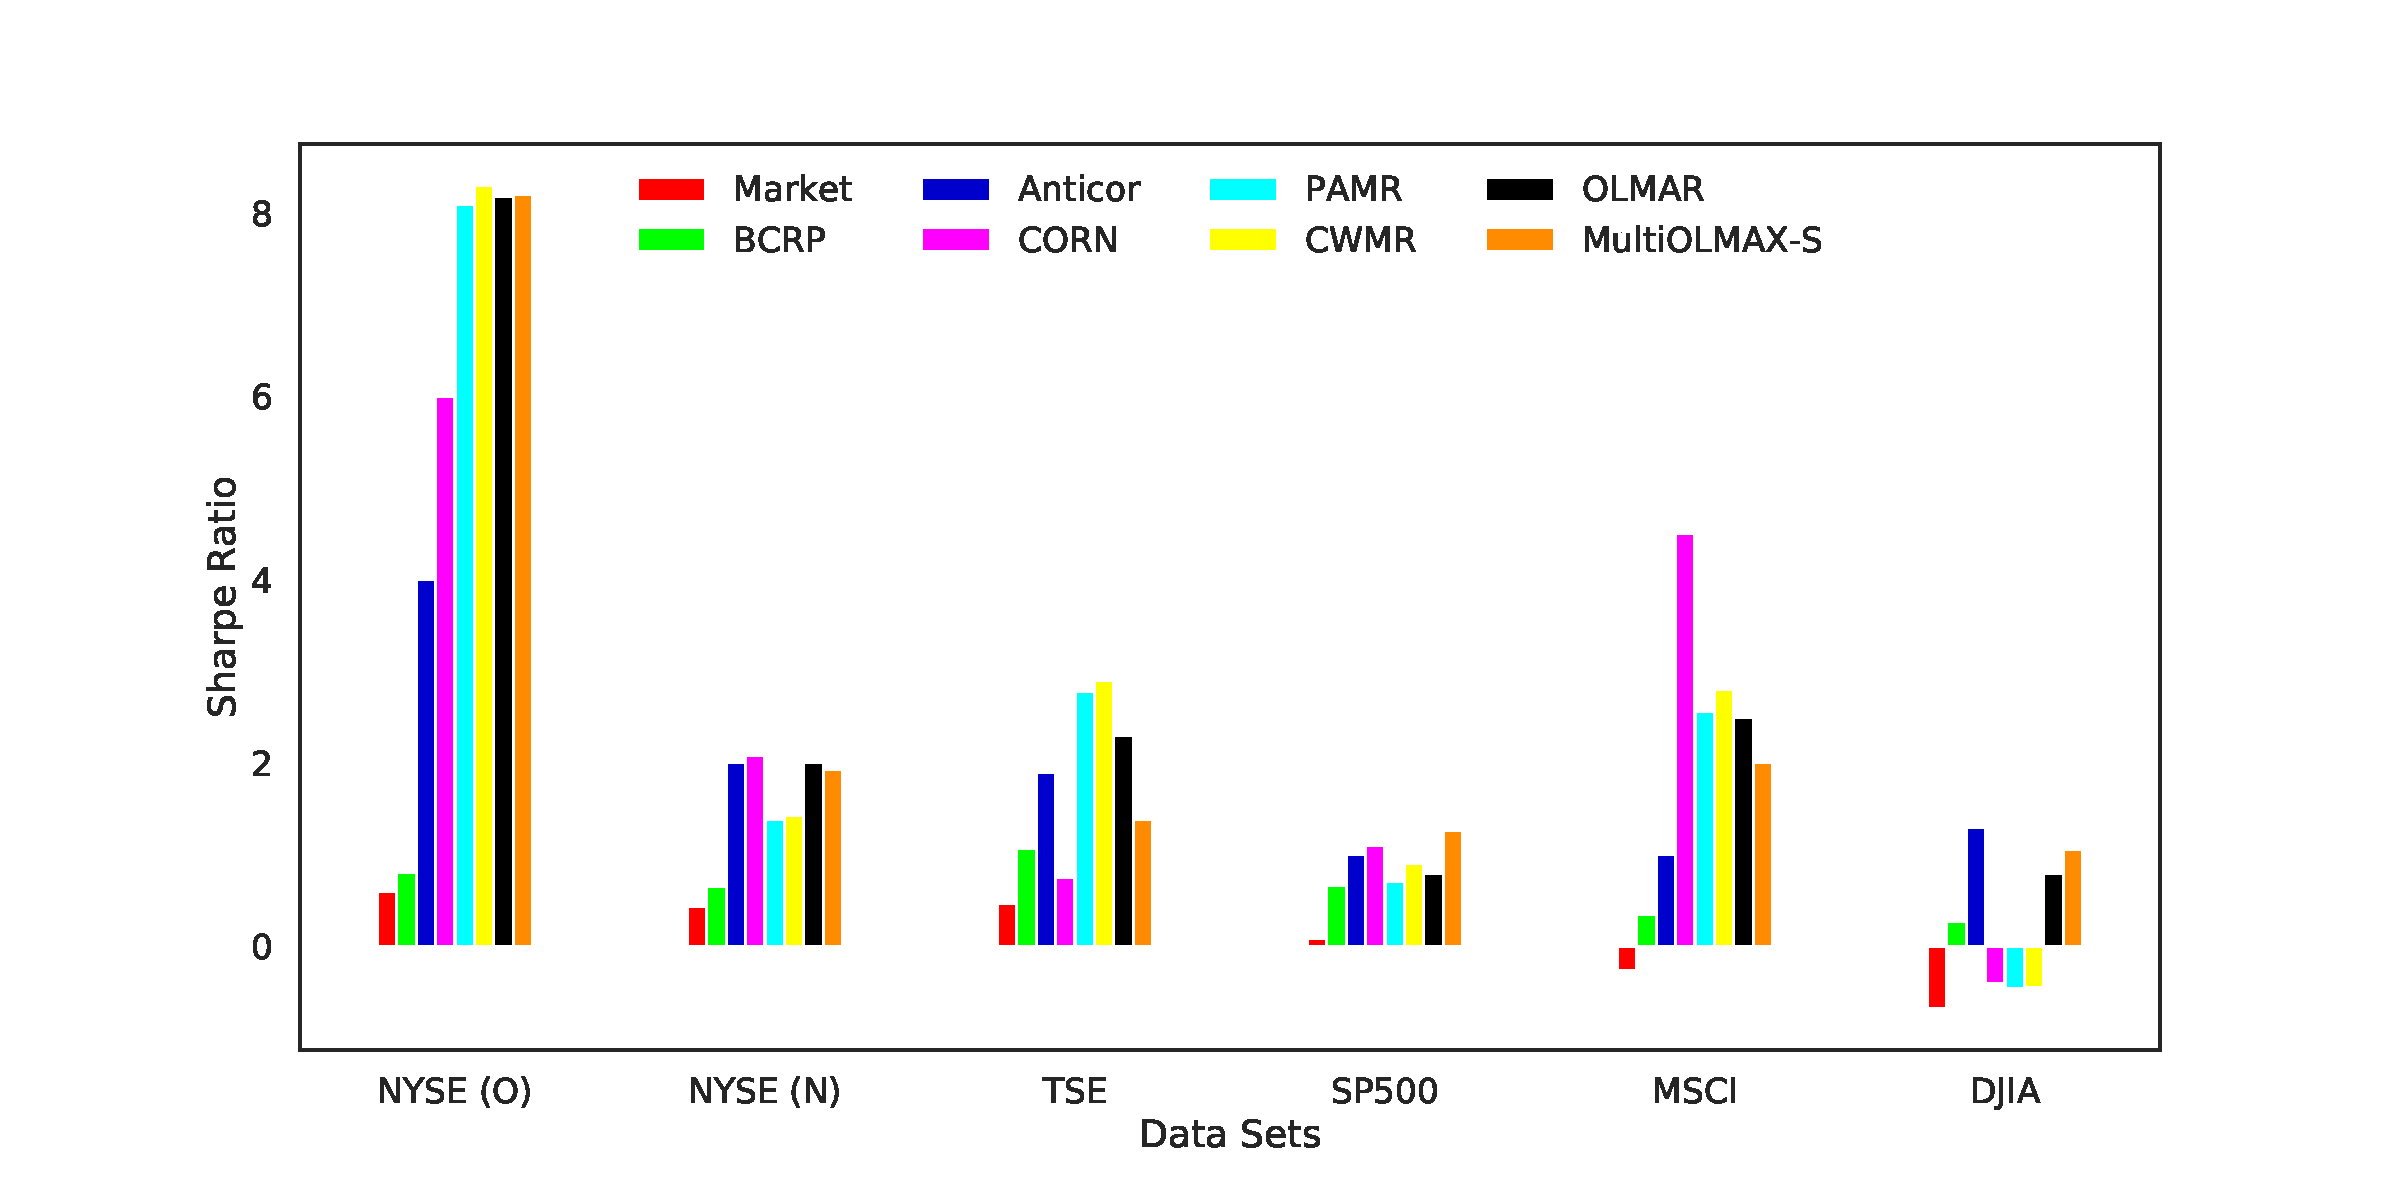
\includegraphics[width=\textwidth,height=\textheight,keepaspectratio]{sharpes}%
}
\end{figure}

\subsection{Hyperparameter sensitivity}
\label{sec:olmax-hyperparameter-sensitivity}

Next we assess the sensitivity of OLMAX with respect to its hyperparameters, namely the lookback window $w$ in the MultiOLMAX-S variant and the smoothing factor $\alpha$ in its MultiOLMAX-E counterpart. These are depicted in Figures~\ref{fig:multiolmax-sensitivity} and~\ref{fig:multiolmax2-sensitivity}, respectively.

From Figure~\ref{fig:multiolmax-sensitivity}, we see that as $w$ increases, the performance deteriorates on the NYSE (O), NYSE (N) and, following an initial spike, the MSCI data sets. As for TSE and SP500, MultiOLMAX-S attains the highest terminal wealth for $w = 35$ and $w = 65$, respectively, while on DJIA we observe a multi-modal pattern. It is remarkable that for most choices of $w$, the total wealth generated by MultiOLMAX-S exceeds that of the Market and BCRP benchmarks by a significant margin.

As for the MultiOLMAX-E variant, we observe in Figure~\ref{fig:multiolmax2-sensitivity} that on most data sets, terminal wealth is consistently high across a wide range of values for $\alpha$, the two extreme endpoints $\alpha = 0$ and $\alpha = 1$ being the exception. We can see why this is so, as follows. If $\alpha = 1$, then all expected price relatives are always 1 and MultiOLMAX-E outputs $\mathbf{b}_{t+1} = \mathbf{b}_t$ on each trading period $t$. Since, by convention, we use the equally-weighted portfolio $\mathbf{1}/m$ for initialisation purposes, this amounts to rebalancing the MultiOLMAX-E portfolio to the equally-weighted one on each trading period, which explains the poor performance. On the other hand, when $\alpha = 0$, the expected vector of price relatives equals $\widetilde{\mathbf{x}}_{t+1} = \frac{1}{\bigotimes_{\tau=1}^{t}\mathbf{x}}_{\tau}}$, i.e.\ it inversely relates to the entire history of price relatives, and should thereby not be expected to produce excellent results.

\begin{figure}%
\caption{Sensitivity of MultiOLMAX-S with respect to its lookback window $w$.}
\label{fig:multiolmax-sensitivity}
    \subfloat[NYSE (O)]{{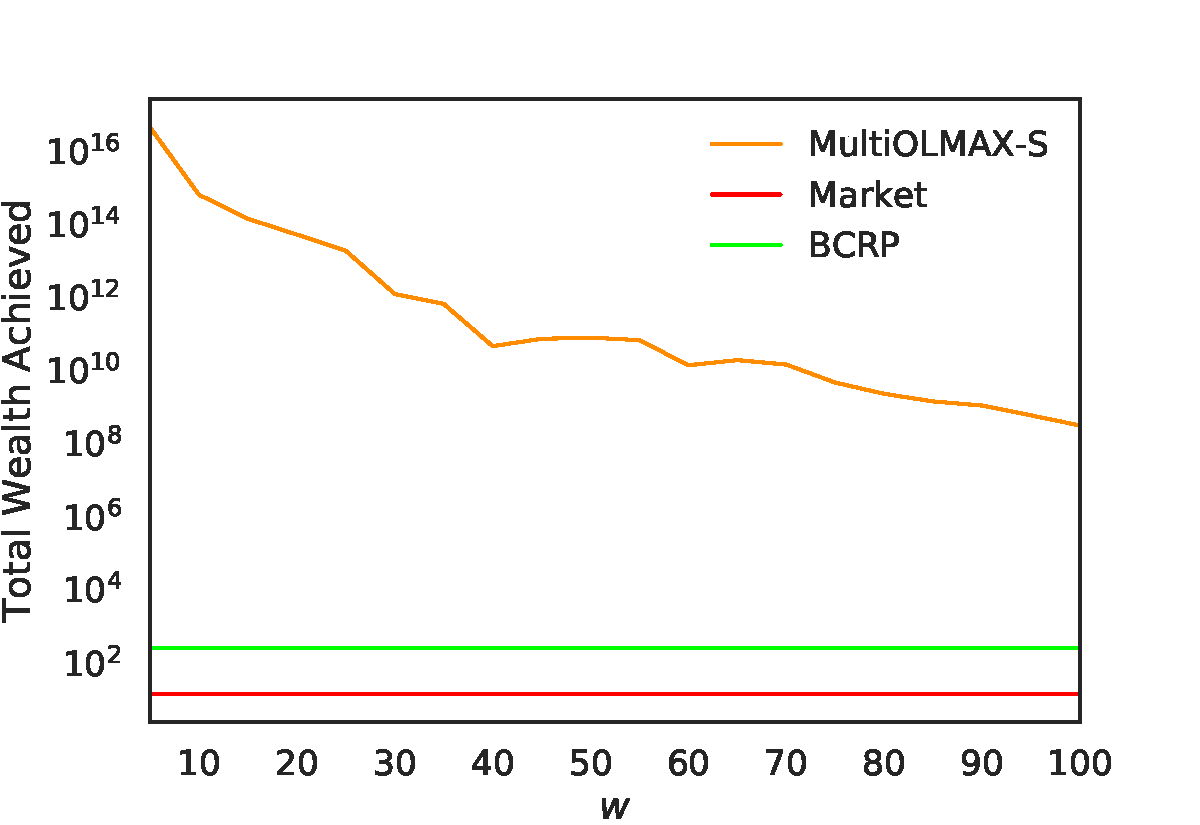
\includegraphics[width=4.5cm, keepaspectratio]{multiolmax-sensitivity_nyse-o} }}%
    \,
    \subfloat[NYSE (N)]{{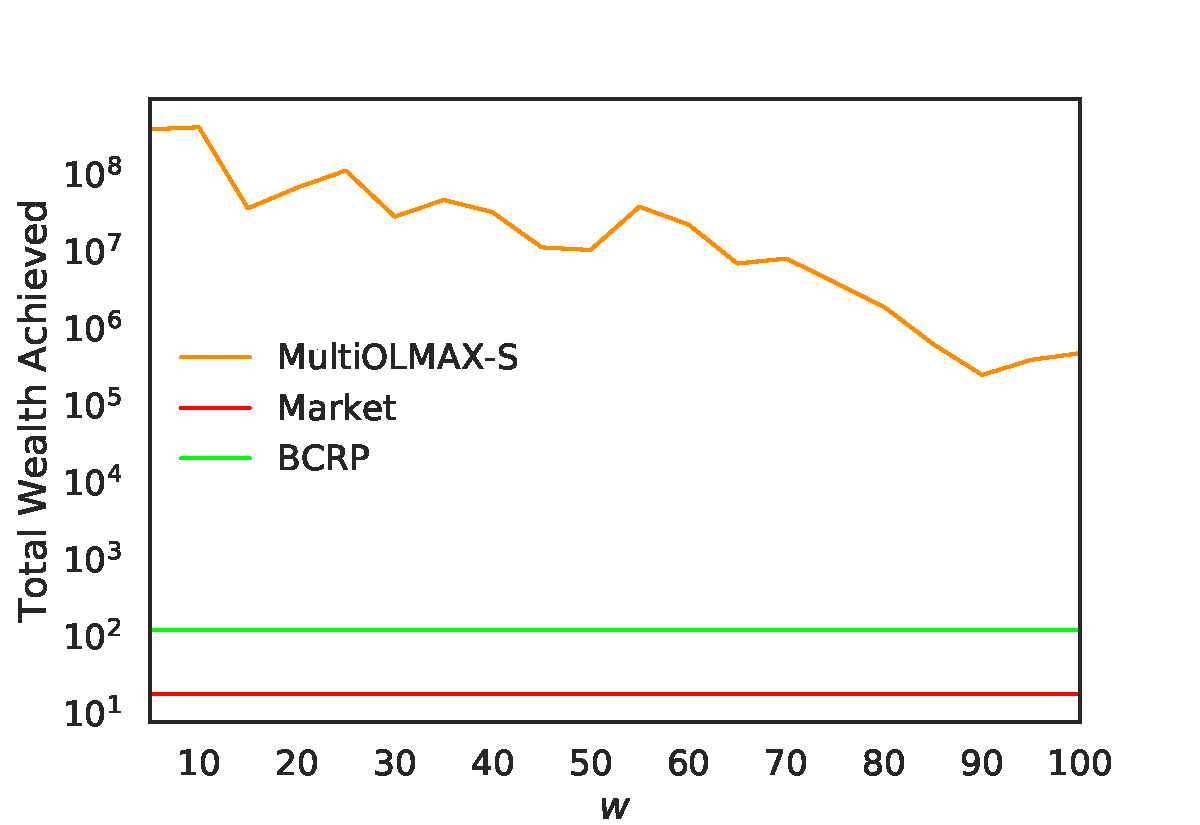
\includegraphics[width=4.5cm, keepaspectratio]{multiolmax-sensitivity_nyse-n} }}%
    \,
    \subfloat[TSE]{{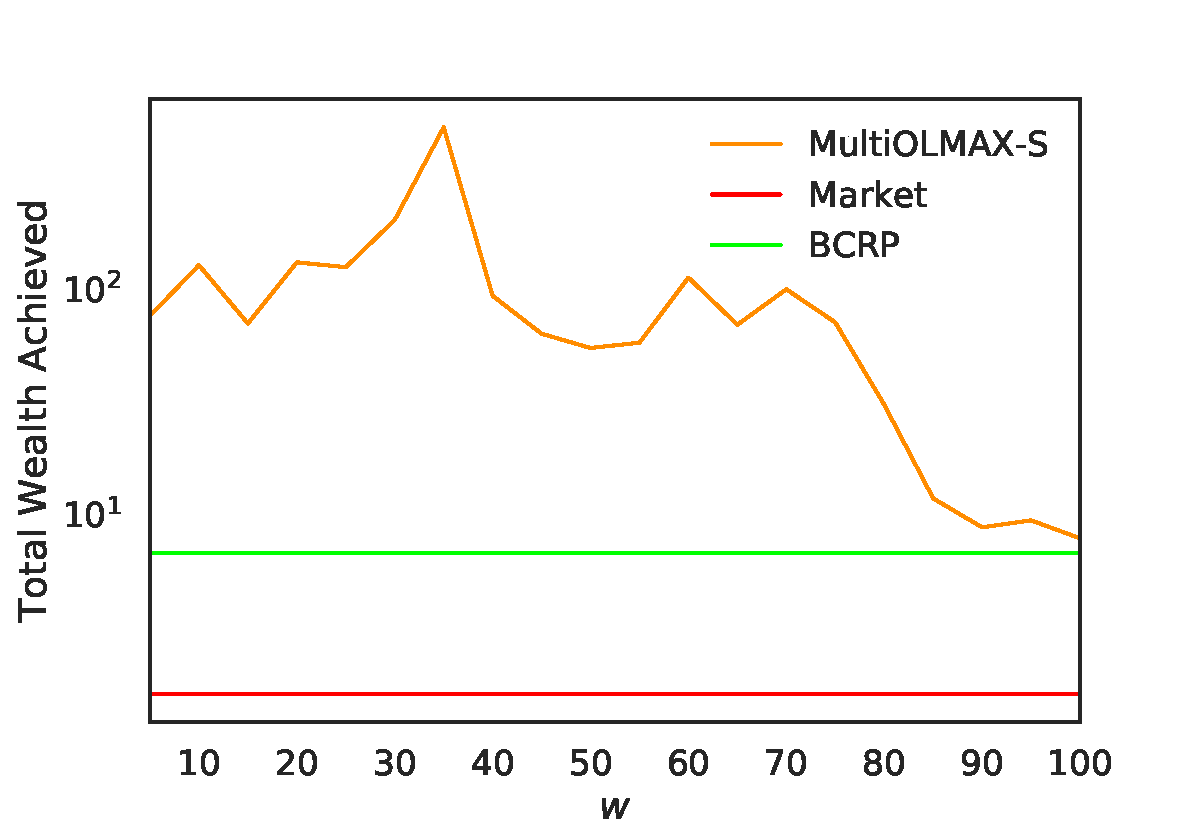
\includegraphics[width=4.5cm, keepaspectratio]{multiolmax-sensitivity_tse} }}%
    
    \subfloat[SP500]{{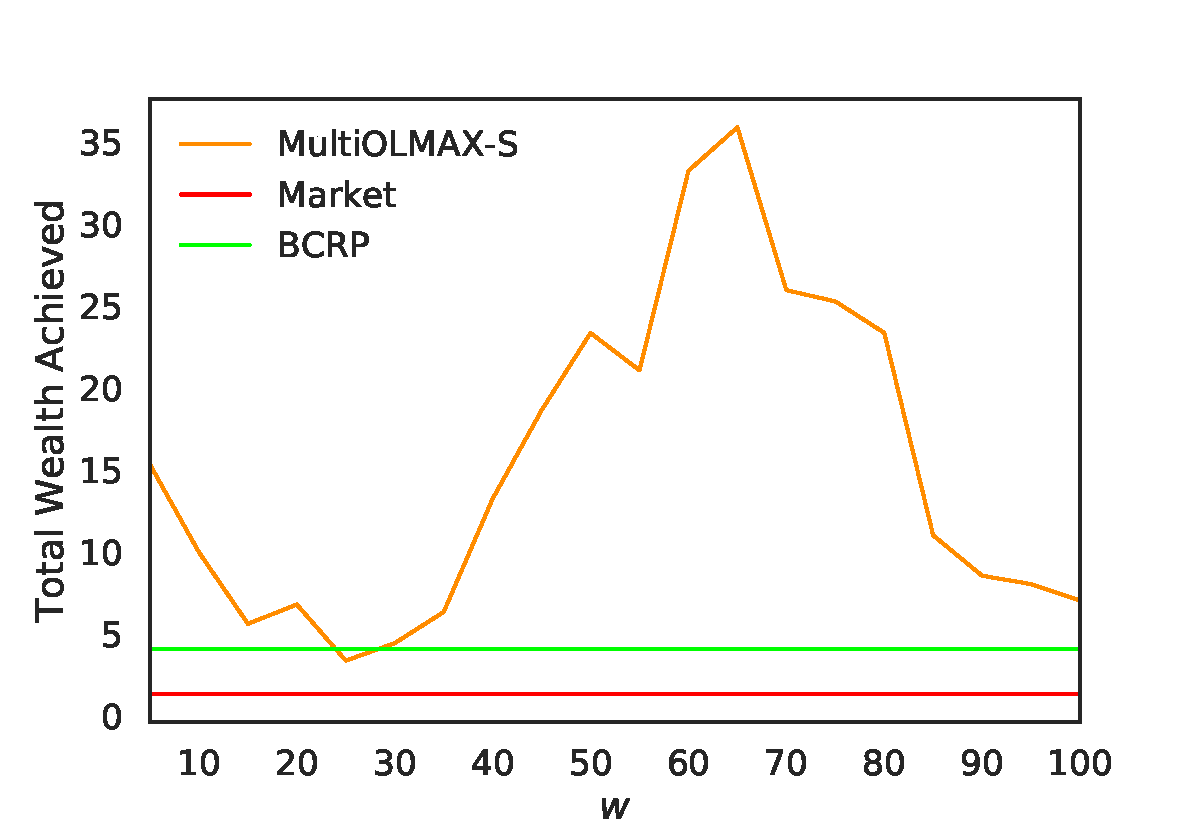
\includegraphics[width=4.5cm, keepaspectratio]{multiolmax-sensitivity_sp500} }}%
    \,
    \subfloat[MSCI]{{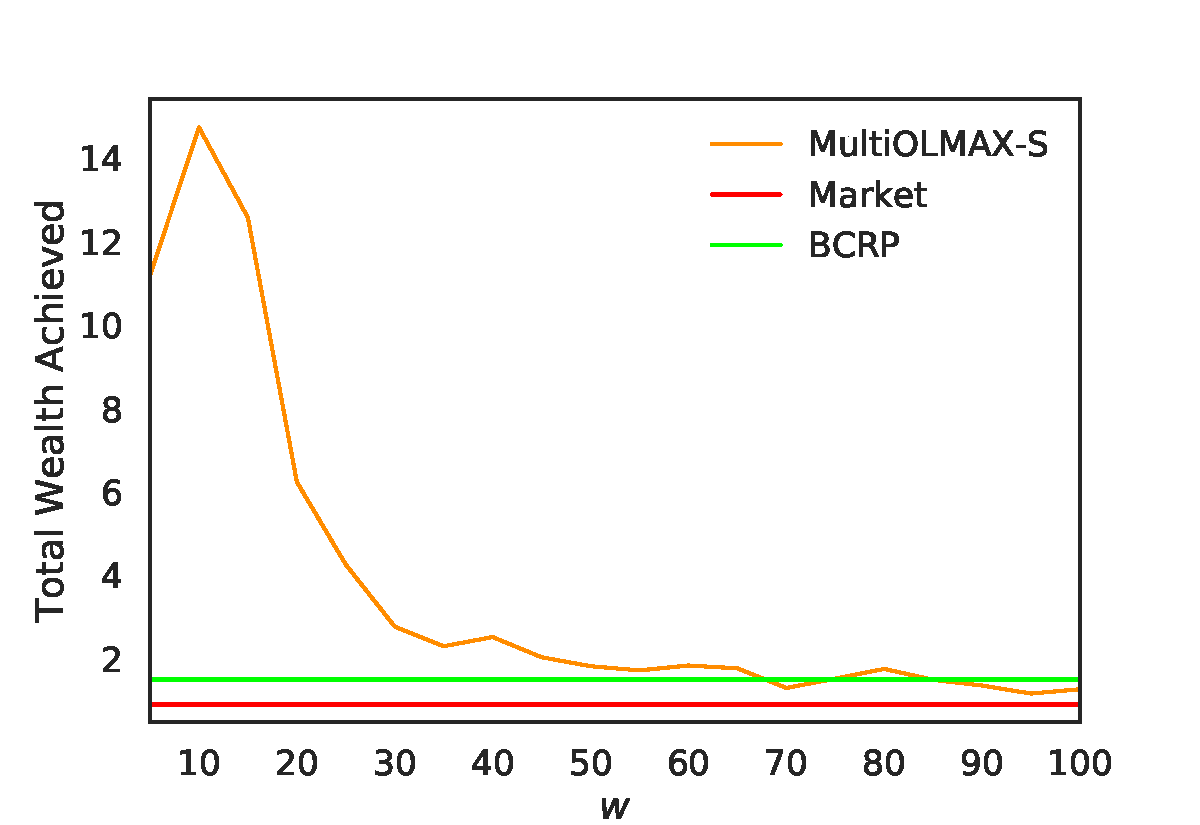
\includegraphics[width=4.5cm, keepaspectratio]{multiolmax-sensitivity_msci} }}%
    \,
    \subfloat[DJIA]{{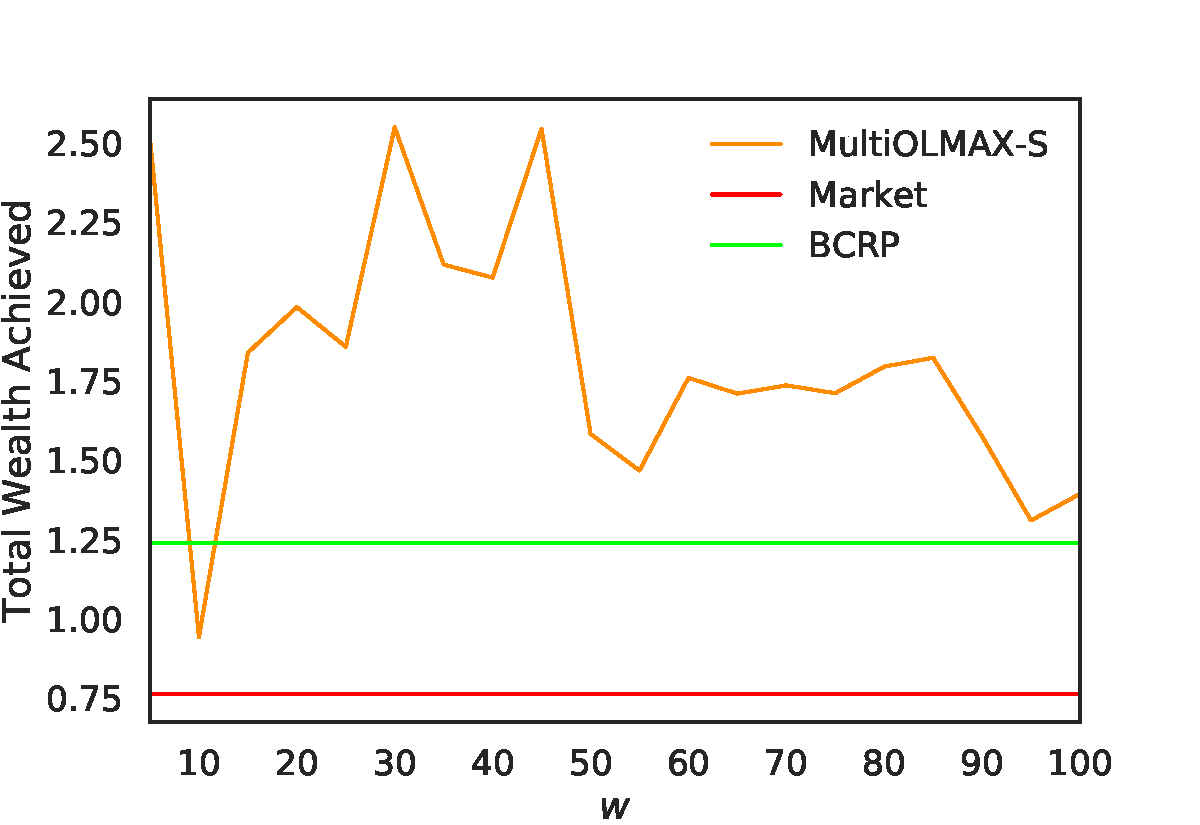
\includegraphics[width=4.5cm, keepaspectratio]{multiolmax-sensitivity_djia} }}%
\end{figure}

\begin{figure}%
\caption{Sensitivity of MultiOLMAX-E with respect to its smoothing factor $\alpha$.}
\label{fig:multiolmax2-sensitivity}
    \subfloat[NYSE (O)]{{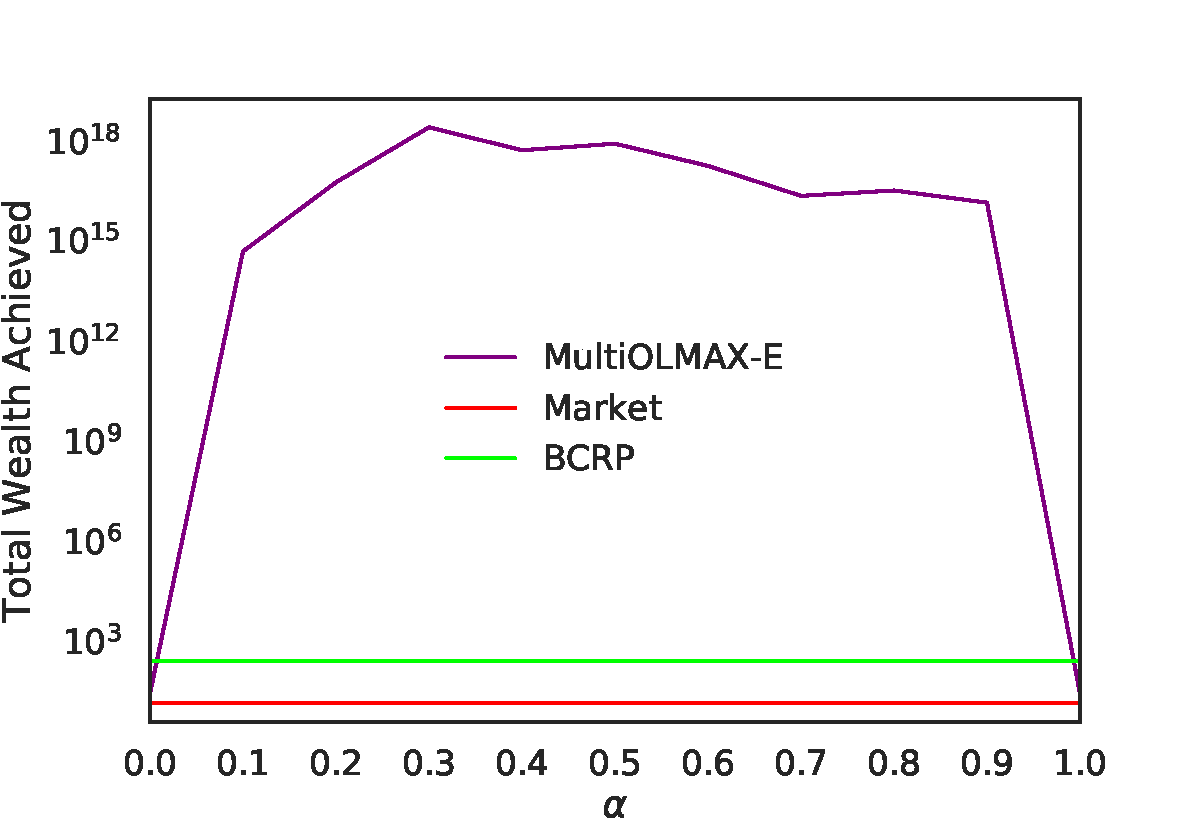
\includegraphics[width=4.5cm, keepaspectratio]{multiolmax2-sensitivity_nyse-o} }}%
    \,
    \subfloat[NYSE (N)]{{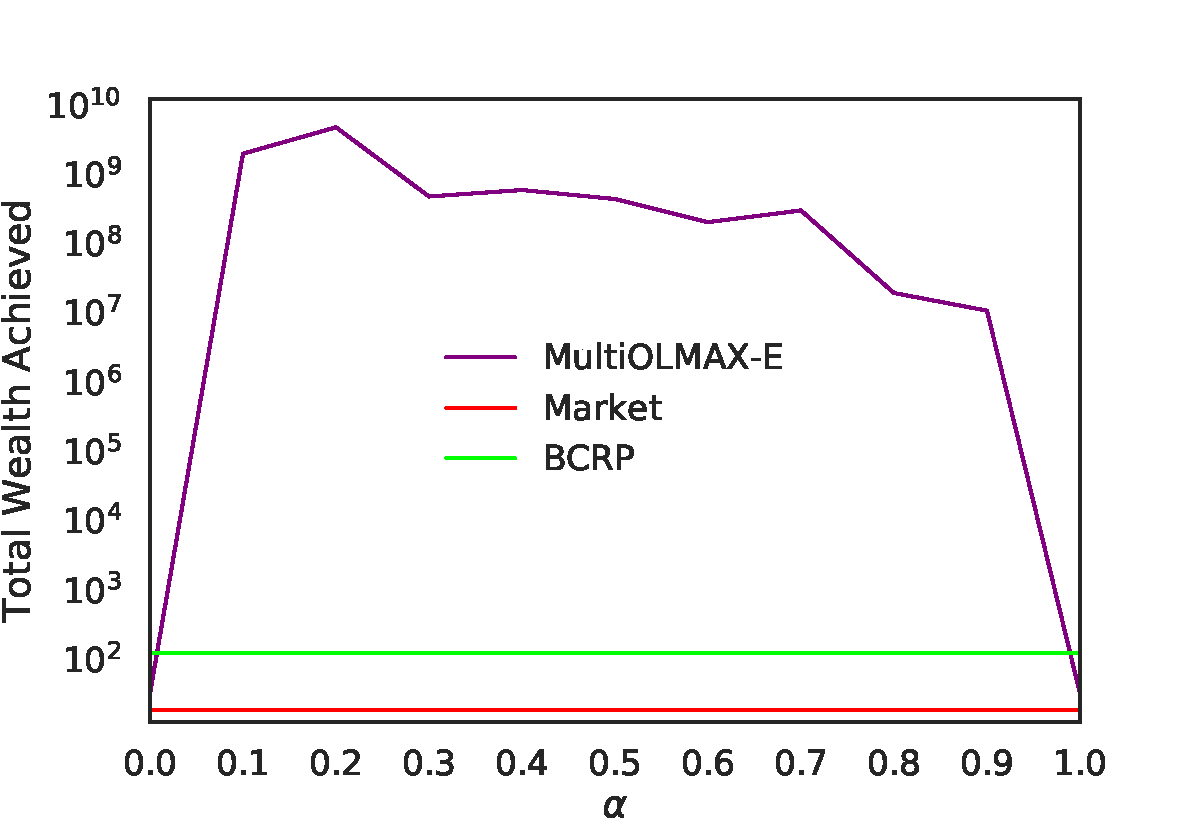
\includegraphics[width=4.5cm, keepaspectratio]{multiolmax2-sensitivity_nyse-n} }}%
    \,
    \subfloat[TSE]{{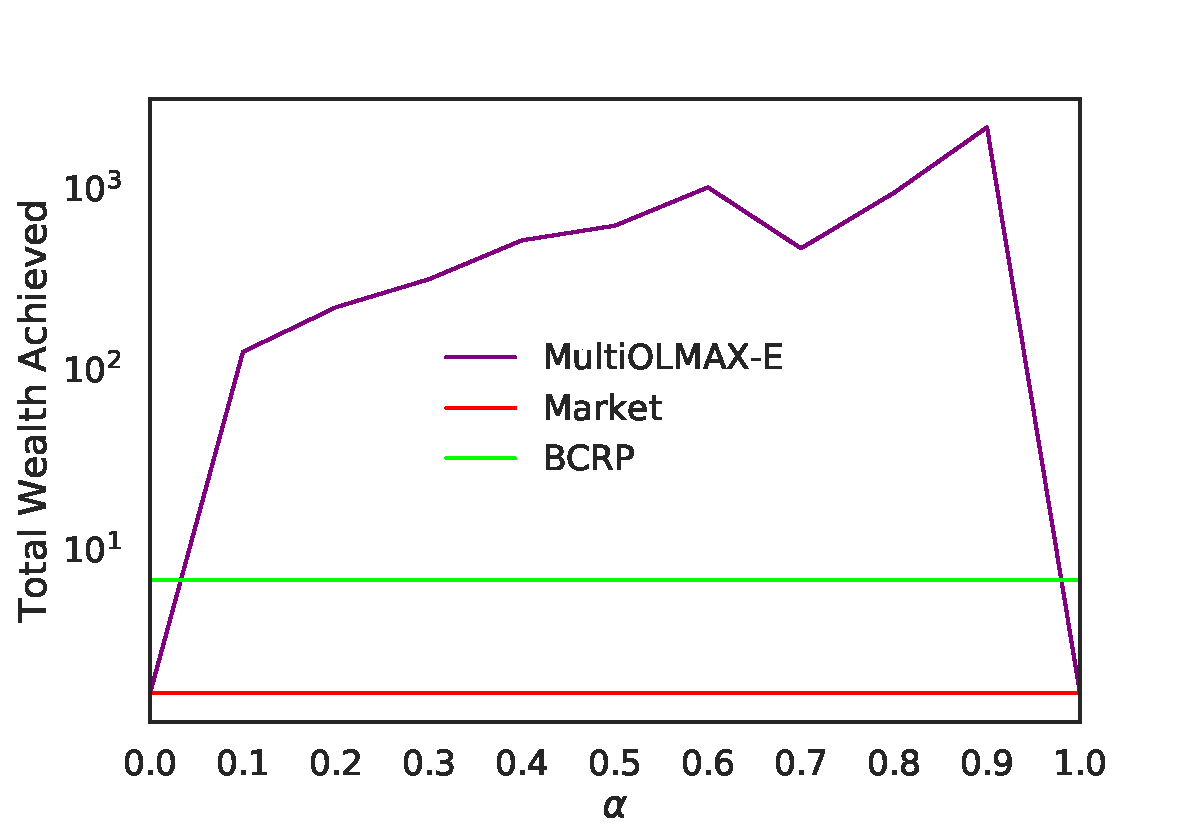
\includegraphics[width=4.5cm, keepaspectratio]{multiolmax2-sensitivity_tse} }}%
    
    \subfloat[SP500]{{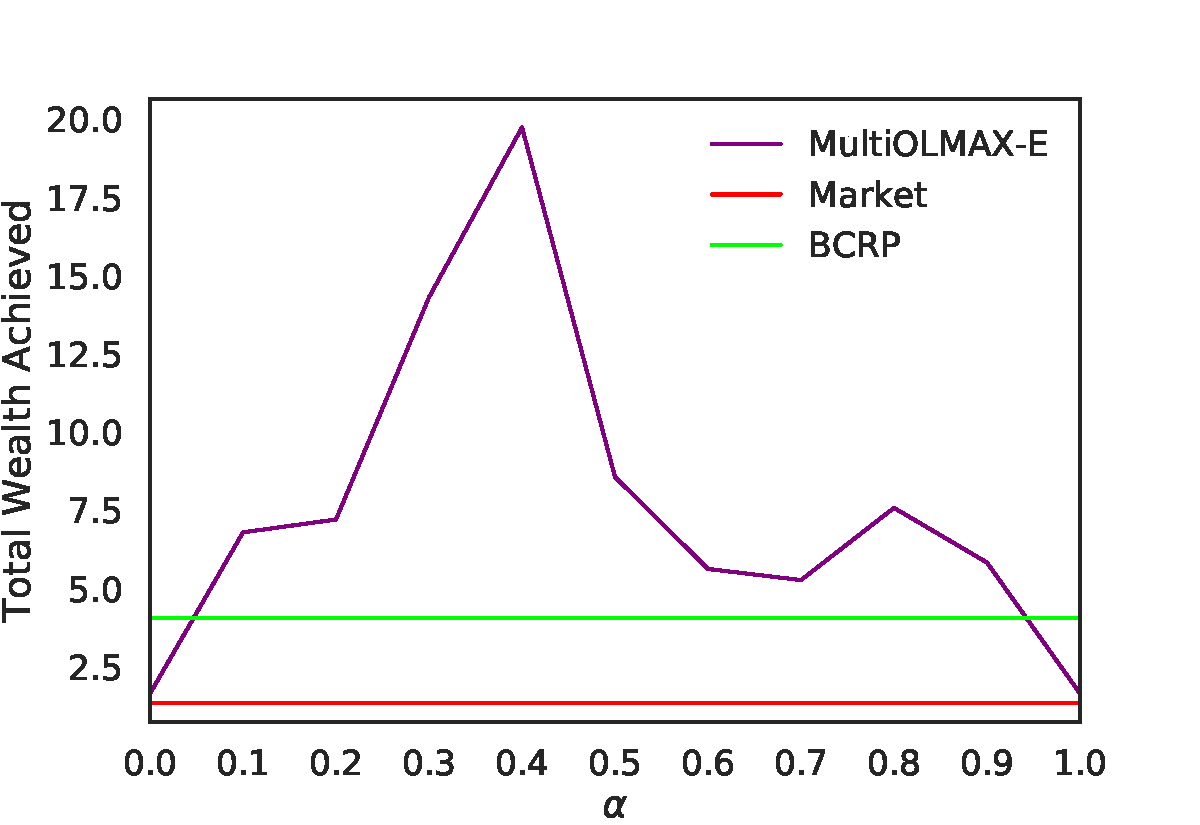
\includegraphics[width=4.5cm, keepaspectratio]{multiolmax2-sensitivity_sp500} }}%
    \,
    \subfloat[MSCI]{{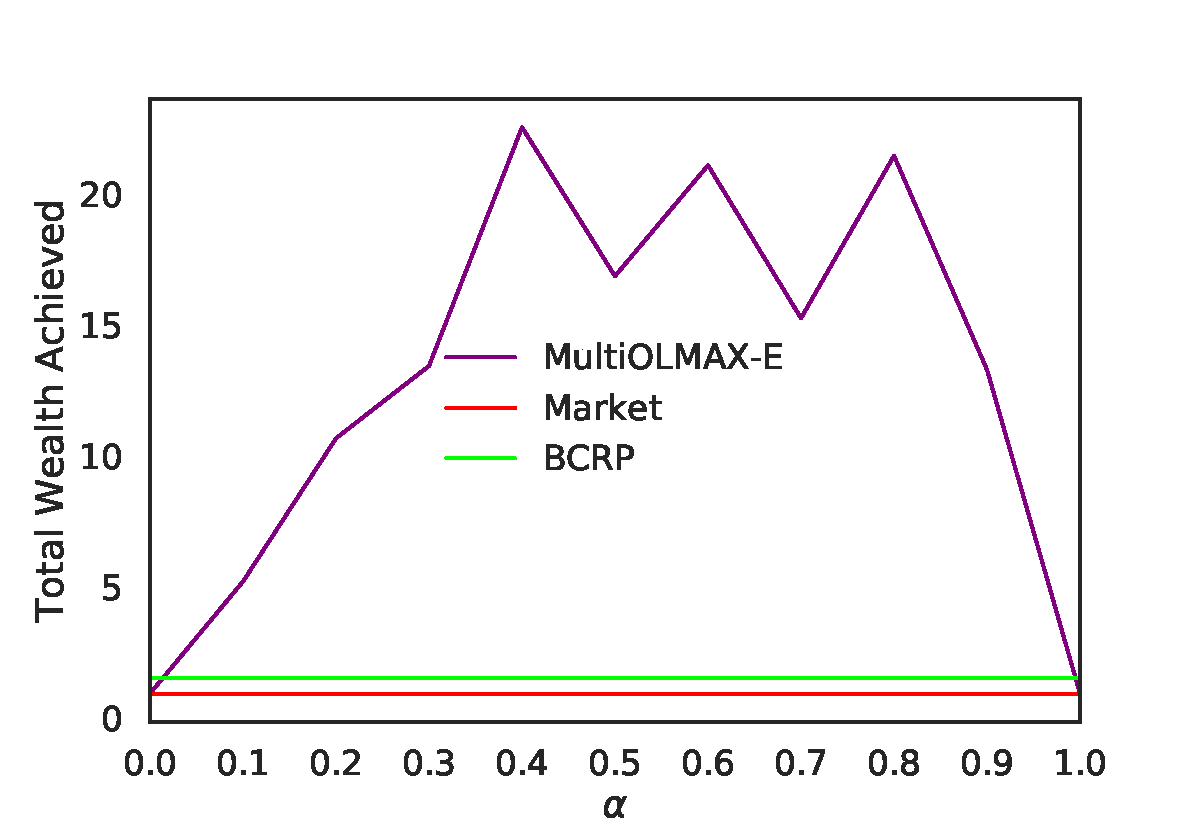
\includegraphics[width=4.5cm, keepaspectratio]{multiolmax2-sensitivity_msci} }}%
    \,
    \subfloat[DJIA]{{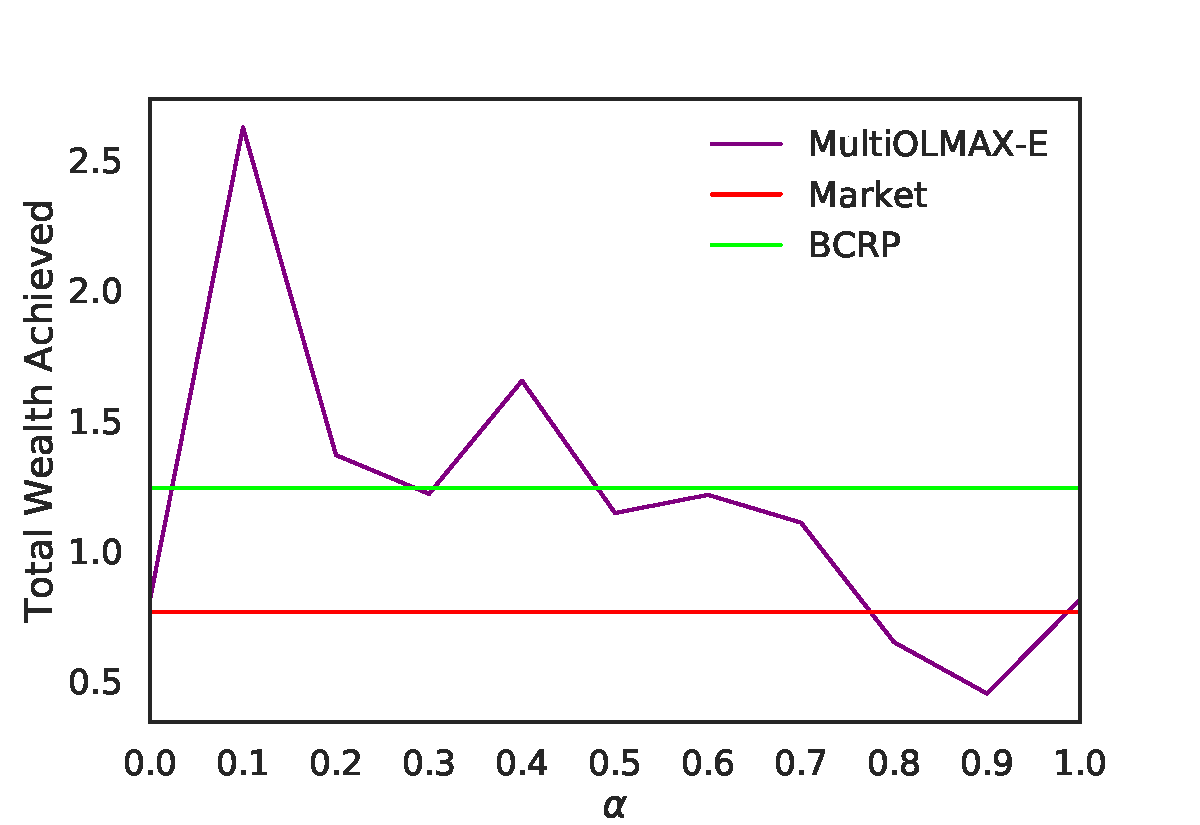
\includegraphics[width=4.5cm, keepaspectratio]{multiolmax2-sensitivity_djia} }}%
\end{figure}

\subsection{Practical performance under transaction costs}
\label{sec:transaction-costs}

To evaluate the practical applicability of the OLMAX framework, we analyse its robustness to proportional transaction fees \citep{borodin04}. Figure~\ref{fig:multiolmax-transaction-cost-sensitivity} illustrates the final wealth achieved by the MultiOLMAX-S method as a function of the transaction-cost rate $\gamma$, along with the corresponding results for the Market and BCRP benchmarks.
\begin{figure}%
\caption{Scalability of the proposed strategy with respect to the transaction-cost rate ($\gamma$).}
\label{fig:multiolmax-transaction-cost-sensitivity}
    \subfloat[NYSE (O)]{{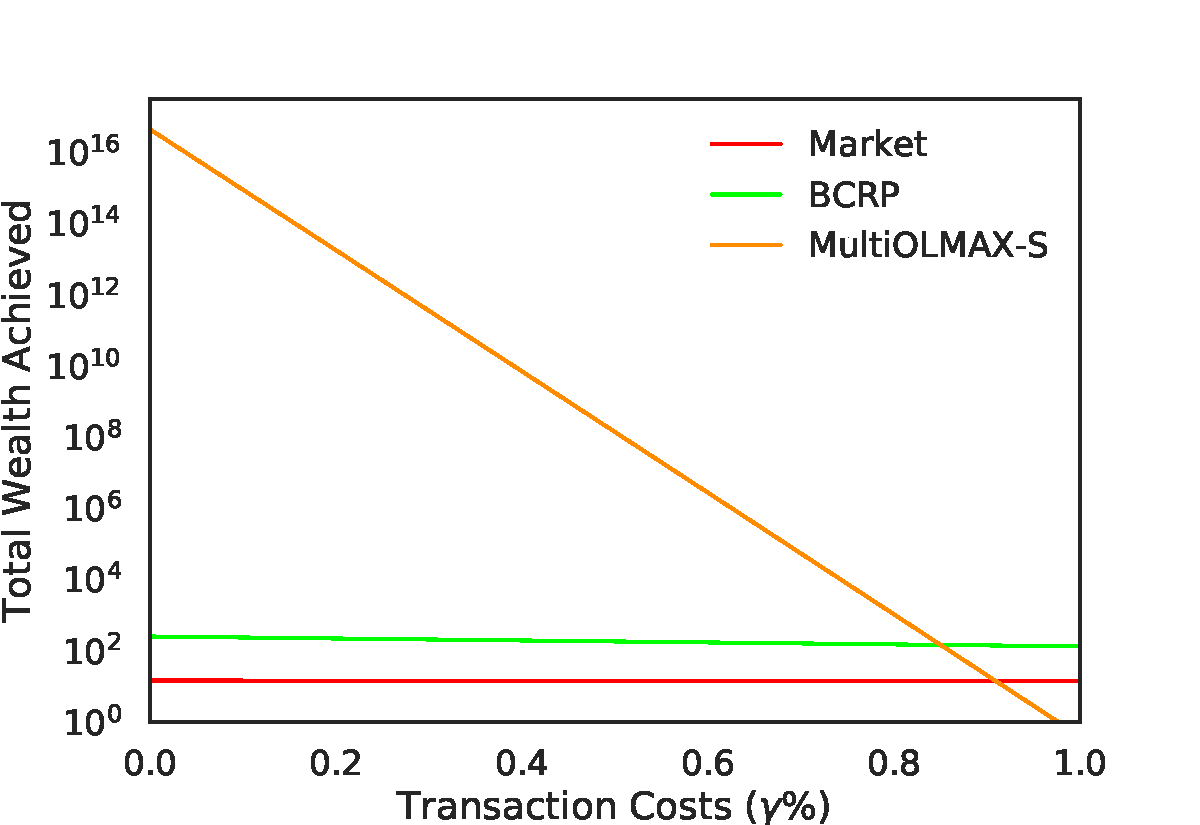
\includegraphics[width=4.5cm, keepaspectratio]{transaction-costs_nyse-o} }}%
    \,
    \subfloat[NYSE (N)]{{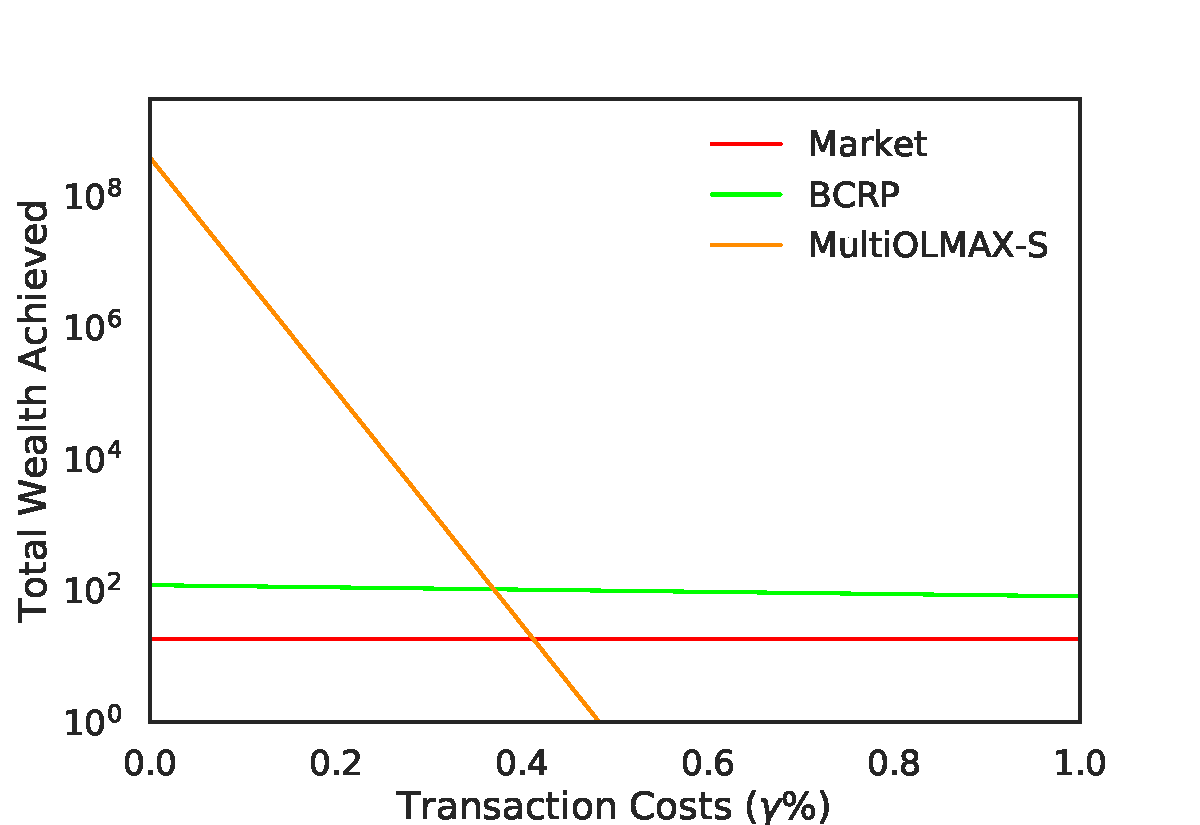
\includegraphics[width=4.5cm, keepaspectratio]{transaction-costs_nyse-n} }}%
    \,
    \subfloat[TSE]{{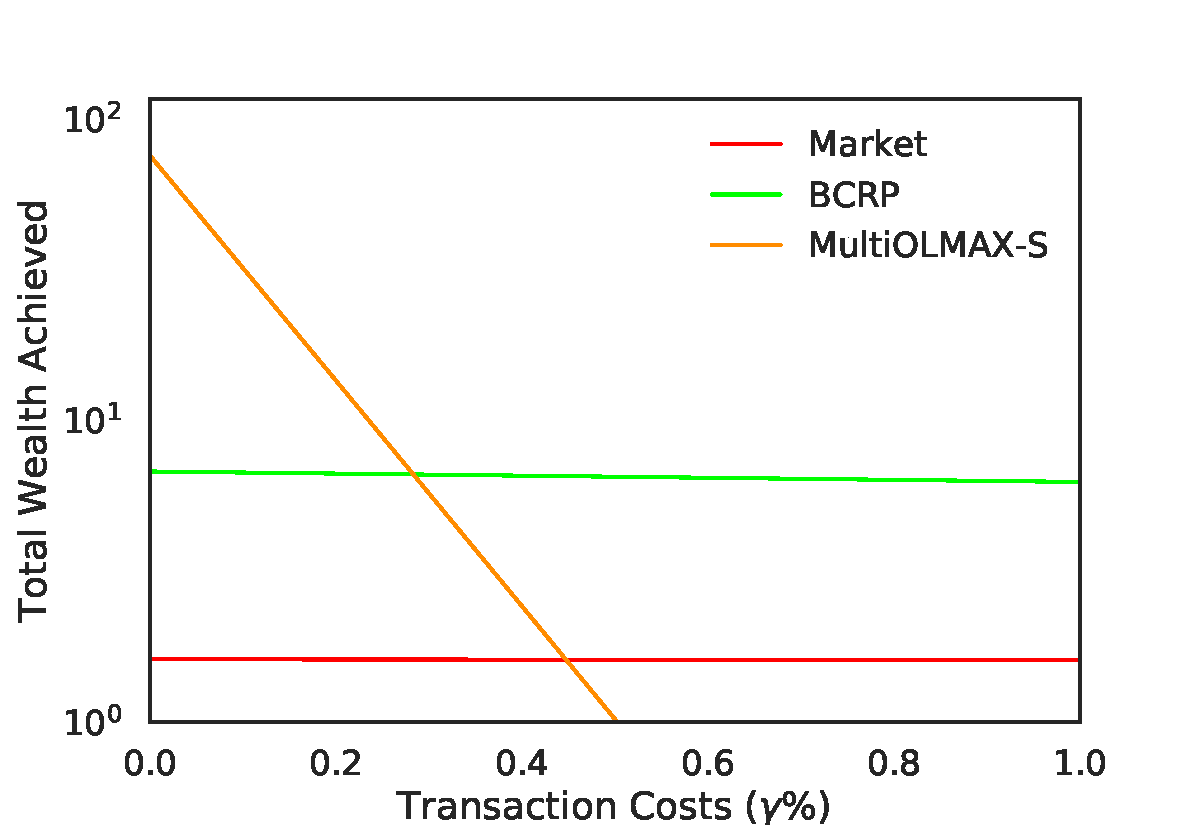
\includegraphics[width=4.5cm, keepaspectratio]{transaction-costs_tse} }}%
    
    \subfloat[SP500]{{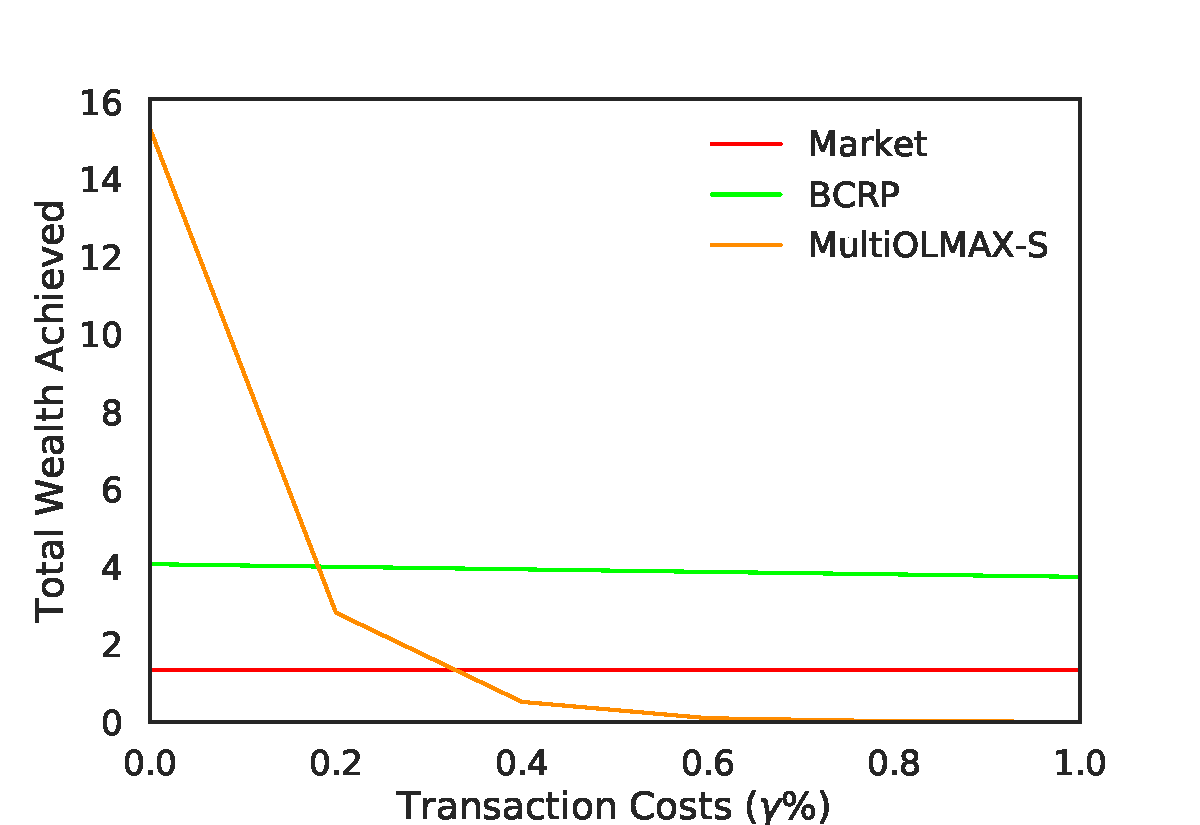
\includegraphics[width=4.5cm, keepaspectratio]{transaction-costs_sp500} }}%
    \,
    \subfloat[MSCI]{{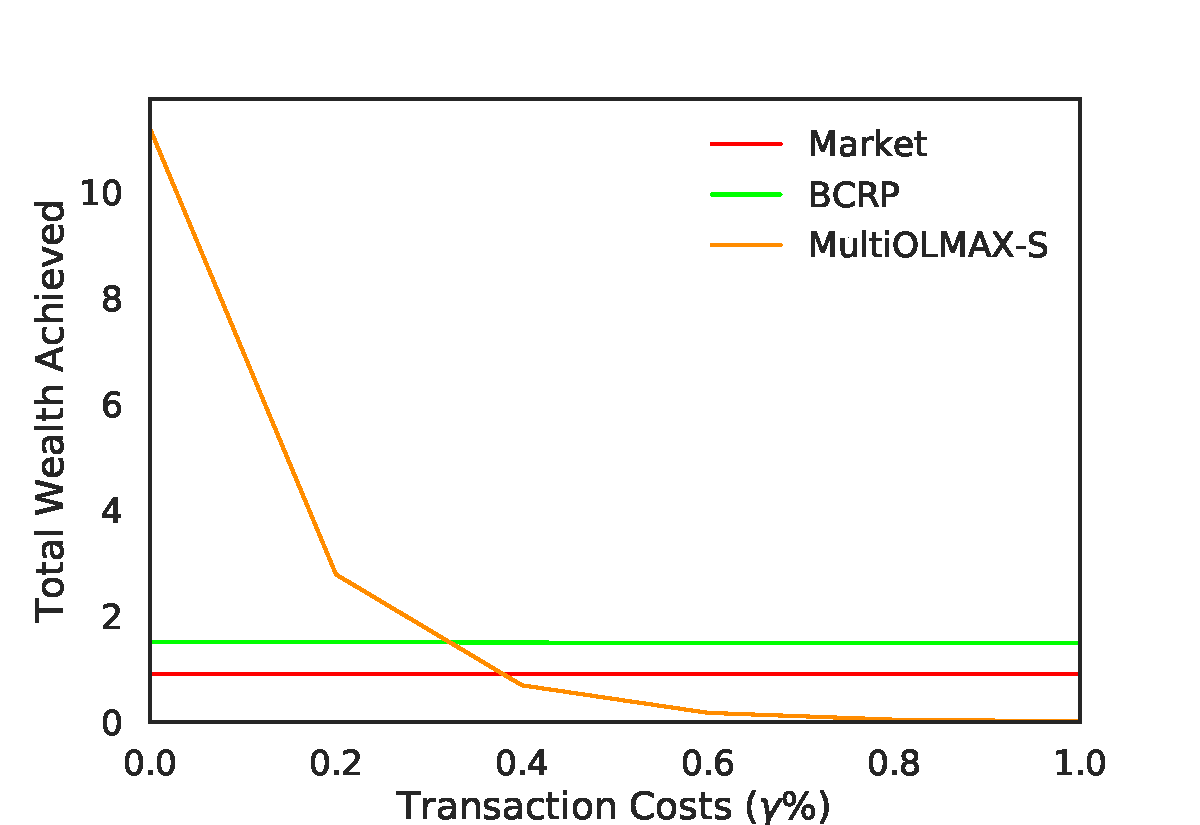
\includegraphics[width=4.5cm, keepaspectratio]{transaction-costs_msci} }}%
    \,
    \subfloat[DJIA]{{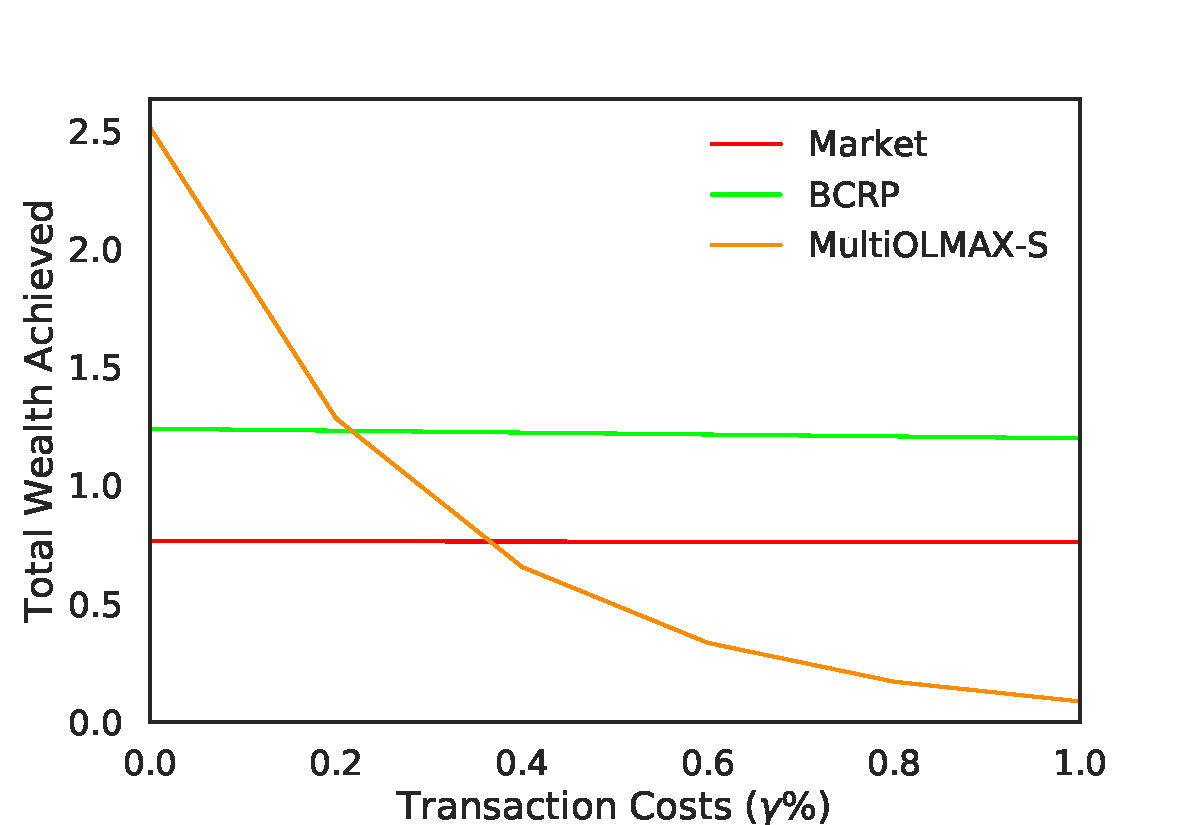
\includegraphics[width=4.5cm, keepaspectratio]{transaction-costs_djia} }}%
\end{figure}

On one hand, Figure~\ref{fig:multiolmax-transaction-cost-sensitivity} clearly shows that MultiOLMAX-S can withstand reasonable transaction costs, as it often has high break-even capability relative to the market. On the other hand, it can outperform the benchmarks under various transaction-cost assumptions. Consequently, MultiOLMAX-S exhibits outstanding performance even when trading is not frictionless, which provides further support to its practical applicability.

%\subsection{Evaluation of computational cost}

\section{Adaptive Online Mean Reversion}
\label{sec:ada-mr}

\subsection{Motivation}

Despite the effectiveness of the proposed OLMAX framework, one cannot help but notice that the corresponding experiments suffer from \emph{selection bias}, in the sense that they fail to cover asset classes other than equities. The same caveat holds for the CWMR, PAMR and OLMAR strategies, among others. The purpose of this subsection is to demonstrate that, in a portfolio that is broadly diversified in terms of asset classes, the aforementioned algorithms no longer exhibit a stellar performance after adding arguably reasonable fees of $0.1\%$ per transaction (corresponding to $\$1$ for every $\$1,000$ of bought/sold asset units). Additionally, we shall perform a sensitivity analysis suggesting that this practical limitation is related to the data-snooping bias from which these strategies suffer.

The first issue that we face concerns the best way to form a diversified portfolio. Since this lies outside the scope of this thesis, we shall simply follow the approach of David Swensen\footnote{David Swensen has been the chief investment officer of Yale University's endowment fund since 1985, and is highly regarded in the asset management community.}, who suggests a portfolio composed of six different asset classes, as follows: US equities (30\% weighting), international equities (15\%), emerging markets (10\%), Treasury inflation-protected securities (TIPS) (15\%), US treasuries (15\%) and real-estate investment trusts (REITs) (15\%) \citep{swensen}. Since we are not concerned with portfolio construction, we will use a set of highly liquid exchange-traded funds (ETFs) as vehicles for these asset classes. These are listed in Table~\ref{tab:etf-dataset}.
\begin{table}[H]
  \caption{Exchange-traded fund (ETF) dataset used in our empirical evaluation. Daily adjusted closing prices for these ETFs were obtained from \href{https://finance.yahoo.com/}{Yahoo! Finance}, for the period from January 1, 2005 until June 3, 2019 inclusive.}
  \label{tab:etf-dataset}
  \centering
  \resizebox{\textwidth}{!}{\begin{tabular}{llccc}
    \toprule
    Ticker & Name & Asset Class & Region & Number of Holdings \\
    \midrule
    VTI & Vanguard Total Stock Market ETF & Equity & US & 3629 \\
    EFA & iShares MSCI EAFE ETF & Equity & Europe, Australia, Asia \& the Far East & 937 \\
    EEM & iShares MSCI Emerging Markets ETF & Equity & Emerging markets & 857 \\
    TLT & iShares 20+ Year Treasury Bond ETF & Fixed Income & US & 30 \\
    TIP & iShares TIPS Bond ETF & Fixed Income & US & 38 \\
    VNQ & Vanguard Real Estate ETF & Equity & US & 184 \\
    \bottomrule
\end{tabular}}
\end{table}

Figure~\ref{fig:etf-cumwealth} clearly illustrates the lack of robustness with respect to transaction costs of PAMR, CWMR, OLMAR, SingleOLMAX and MultiOLMAX\footnote{Henceforth, the acronym `MultiOLMAX' will be used as a shorthand for the MultiOLMAX-S strategy, whose price-relative forecasts are based on simple moving averages.}. Under the absence of transaction costs, these methods exhibit decent performance in terms of cumulative wealth, and even exceed the benchmarks (including Swensen's recommended portfolio) by a highly significant margin. However, the picture changes drastically when one introduces fees of 0.1\% per transaction, and none of these algorithms manages to beat any of the benchmarks. Worse, they all stagnate around 2010 and their performance starts deteriorating in 2011 or a couple of years thereafter.
\begin{figure}[H]
    \subfloat[Without fees]{{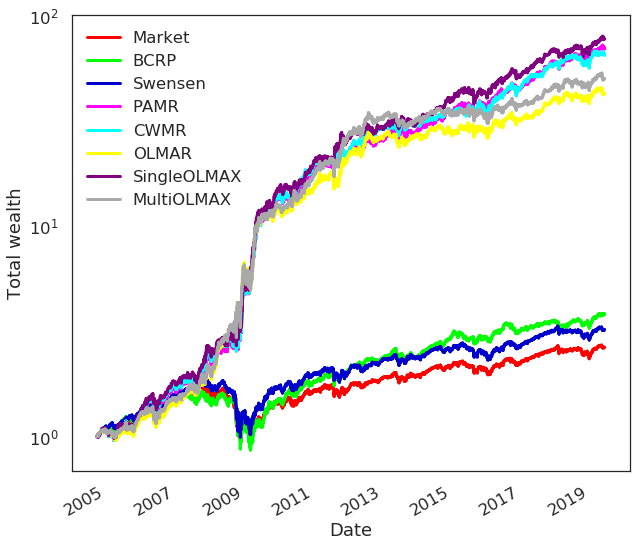
\includegraphics[width=0.5\textwidth, keepaspectratio]{etf-cumwealth-no-fees} }}%
    \,
    \subfloat[Subject to fees of 0.1\%]{{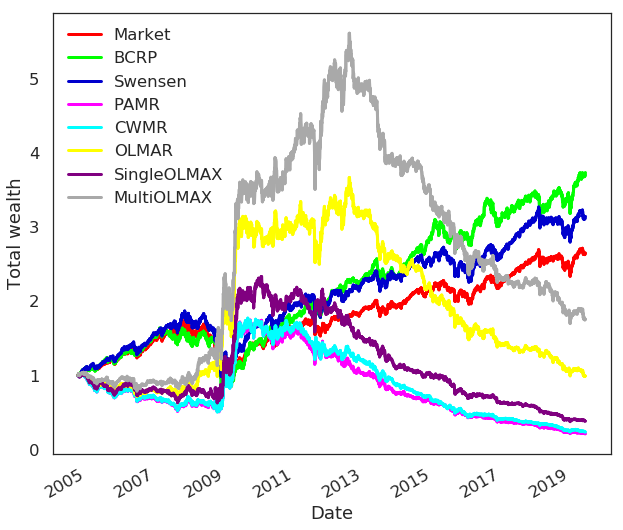
\includegraphics[width=0.5\textwidth, keepaspectratio]{etf-cumwealth-with-fees} }}%
\caption{Trends of cumulative wealth achieved by various strategies during the entire trading periods associated with the ETF data set (see Table~\ref{tab:etf-dataset}). Panel \textbf{(a)} illustrates these trends under the assumption of no transaction costs, whereas panel \textbf{(b)} depicts them net of fees of 0.1\% per transaction.}
\label{fig:etf-cumwealth}
\end{figure}

A deeper analysis reveals that the underperformance documented above may be due to data-snooping bias. Let us focus on OLMAR, for the sake of argument. In Figure~\ref{fig:olmar-sensitivity}, we see with hindsight that the optimal terminal wealth does not occur at the default values $\epsilon = 10$ and $w = 5$ of the underlying parameters, where, as a reminder, $\epsilon$ is the reversion threshold and $w$ the lookback window used in the computation of the price-relative forecasts. For instance, if we keep $\epsilon$ fixed at 10, the optimal window yielding the highest final wealth is $w = 20$. Once we implement the OLMAR algorithm with these parameter values optimised with the benefit of hindsight, we are able to improve its \emph{net} performance (i.e.\ net of transaction fees) beyond that of the benchmarks, as illustrated in Figure~\ref{fig:optimised-olmar}.

\begin{figure}[H]
\caption{Parameter sensitivity of OLMAR on the ETF data set, with respect to \textbf{(a)} $\epsilon$ with fixed $w$ ($w = 5$) and \textbf{(b)} $w$ with fixed $\epsilon$ ($\epsilon = 10$).}
\label{fig:olmar-sensitivity}
    \subfloat[]{{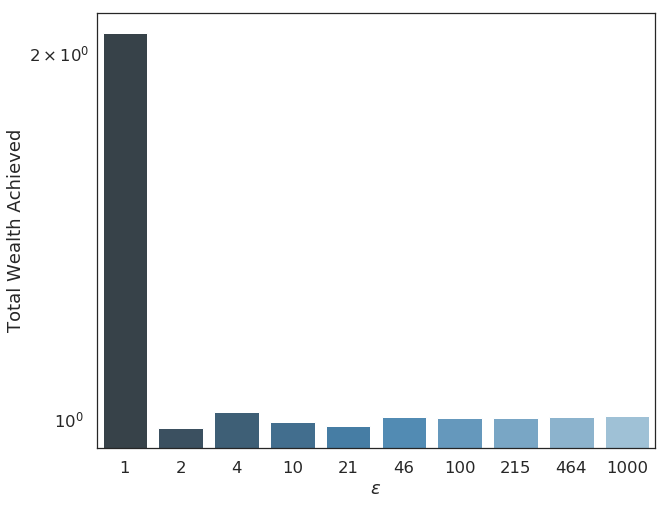
\includegraphics[width=0.5\textwidth, keepaspectratio]{olmar-sensitivity-epsilon_etfs} }}%
    \subfloat[]{{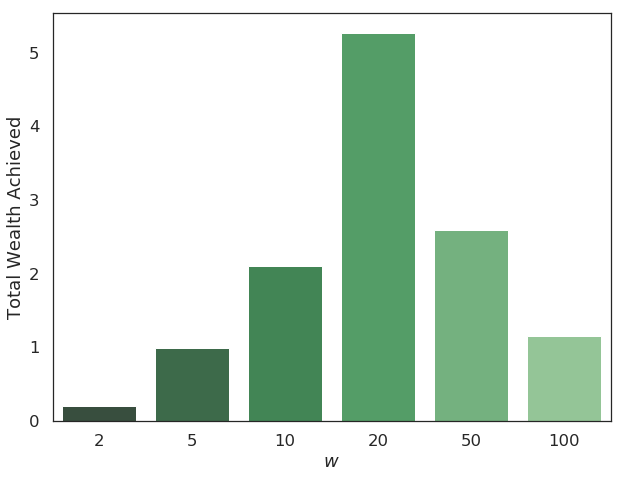
\includegraphics[width=0.5\textwidth, keepaspectratio]{olmar-sensitivity-window_etfs} }}%
\end{figure}

\begin{figure}[H]
\centering
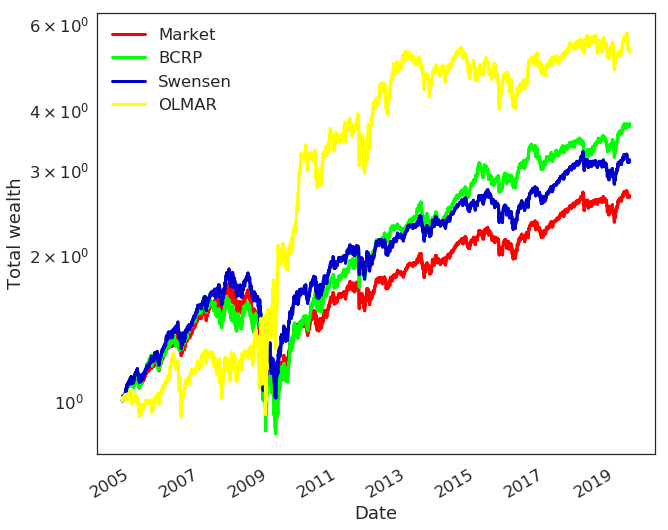
\includegraphics[width=\textwidth, height=\textheight, keepaspectratio]{etf-cumwealth-optolmar-with-fees}
\caption{Cumulative wealth achieved by OLMAR optimised in hindsight (with parameters $\epsilon = 10$ and $w = 20$) vs benchmarks on the ETF data set, subject to transaction fees of 0.1\%.}
\label{fig:optimised-olmar}
\end{figure}

\subsection{Proposed algorithms}

Armed with the insights from Figures~\ref{fig:olmar-sensitivity} and~\ref{fig:optimised-olmar}, we turn now to explore \emph{adaptive} variants of PAMR and OLMAR that are governed by no and a smaller number of hyperparameters, respectively. To this end, we cast the underlying optimisation problems into a, roughly speaking, equivalent OGD-criterion representation (see Eq. \eqref{eq:ogd-criterion}) whose learning rate can be made adaptive via the application of the MAPGRAD algorithm (i.e.\ Algorithm~\ref{alg:mapgrad}).

To start with, let us consider the PAMR strategy. As proposed in \citep{pamr}, the standard variant is formulated as the following constrained optimisation problem:
\begin{equation}
\label{eq:pamr-optpb}
	\min_{\mathbf{b}\in\Delta_m} \; \frac{1}{2}\Vert\mathbf{b} - \mathbf{b}_t\Vert_2^2
	\qquad \text{s.t.} \qquad \mathbf{b} \cdot \mathbf{x}_t \leq \epsilon,
\end{equation}
for $t \in [T-1]$, with the convention $\mathbf{b}_1 = \mathbf{1} / m$. Instead of this problem, we will consider the following proximal problem:
\begin{equation}
\label{eq:pamr-optpb-ogdform}
	\min_{\mathbf{b}\in\Delta_m} \; \Big\{\eta(\mathbf{b} \cdot \mathbf{x}_t) + \frac{1}{2}\Vert\mathbf{b} - \mathbf{b}_t\Vert_2^2\Big\}
	= \min_{\mathbf{b}\in\Delta_m} \; \Big\{\mathbf{b} \cdot \mathbf{x}_t + \frac{1}{2\eta}\Vert\mathbf{b} - \mathbf{b}_t\Vert_2^2\Big\},
\end{equation}
for some $\eta > 0$.
Roughly speaking, the PAMR problem \eqref{eq:pamr-optpb} and the proximal problem \eqref{eq:pamr-optpb-ogdform} have the same solutions for appropriate choices of the parameters $\epsilon$ and $\eta$.
%More precisely, every solution of the proximal problem \eqref{eq:pamr-optpb-ogdform} is also a solution of the PAMR problem \eqref{eq:pamr-optpb} for some choice of $\epsilon$. Conversely, every solution of the PAMR problem \eqref{eq:pamr-optpb} is either a minimiser of
However, the formulation \eqref{eq:pamr-optpb-ogdform} has the form of the OGD criterion in Eq. \eqref{eq:ogd-criterion}, meaning the portfolio weights that solve \eqref{eq:pamr-optpb-ogdform} satisfy the OGD update rule \eqref{eq:ogd}:
\begin{equation}
\label{eq:pamr-portfolio}
	\mathbf{b}_{t+1} = \Pi_{\Delta_m}(\mathbf{b}_t - \eta\mathbf{x}_t),
\end{equation}
where, as a reminder, $\Pi_{\Delta_m}(\mathbf{b})$ signifies the point in $\Delta_m$ that is closest to $\mathbf{b}$.
In order to marginalise the dependence on $\eta$ of the portfolio updates in Eq. \eqref{eq:pamr-portfolio}, we employ the MAPGRAD method outlined in Algorithm~\ref{alg:mapgrad}. The latter prescribes the data-dependent learning-rate schedule $\{\eta_t = m / \Vert\sum_{\tau=1}^{t}\mathbf{x}_\tau\Vert^2_2\,\}_{t=1}^{T-1}$ which, when plugged into Eq. \eqref{eq:pamr-portfolio}, yields the strategy
\begin{equation}
\label{eq:adapamr-portfolio}
	\mathbf{b}_{t+1}
	= \Pi_{\Delta_m}\left(\mathbf{b}_t - \frac{m}{\Vert\sum_{\tau=1}^{t}\mathbf{x}_\tau\Vert^2_2}\,\mathbf{x}_t\right),
	\qquad t \in [T-1],
\end{equation}
subject to the initialisation condition $\mathbf{b}_1 = \mathbf{1} / m$.
For obvious reasons, we shall refer to the latter as \emph{adaptive passive-aggressive mean reversion} strategy, or AdaPAMR for short. The procedure is outlined in Algorithm~\ref{alg:adapamr}.
\begin{algorithm}
  \caption{AdaPAMR: Adaptive Passive-Aggressive Mean Reversion}
\label{alg:adapamr}
  \begin{algorithmic}[1]
    \STATE {\bfseries Initialisation:} initial portfolio $\mathbf{b}_1 = \frac{\mathbf{1}}{m}$, initial wealth $S_0 = 1$, initial gradient sum $\boldsymbol{\theta}_0 = \mathbf{0}$
    \FOR{$t=1, 2, \ldots, T$}
      \STATE observe stock price relatives $\mathbf{x}_t$
      \STATE update wealth:
        $
          S_t = S_{t-1} \times (\mathbf{b}_t^\text{T}\mathbf{x}_t)
        $
      \IF {$t < T$}
        \STATE update the gradient sum: $\boldsymbol{\theta}_t = \boldsymbol{\theta}_{t-1} + \mathbf{x}_t$
        \STATE compute the learning rate:
        \begin{equation*}
        	\eta_t = \frac{m}{\Vert\boldsymbol{\theta}_{t}\Vert^2_2}
        \end{equation*}
        \STATE update the portfolio:
	\begin{equation*}
		\mathbf{b}_{t+1} = 	\mathbf{b}_{t} - \eta_t\mathbf{x}_t
	\end{equation*}
		\STATE normalise the portfolio:
		\begin{equation*}
			\mathbf{b}_{t+1} = \Pi_{\Delta_m}(\mathbf{b}_{t+1})
			= \argmin_{\mathbf{b}\in\Delta_m} \; \Vert\mathbf{b} - \mathbf{b}_{t+1}\Vert_2^2
		\end{equation*}
	\ENDIF
    \ENDFOR
  \end{algorithmic}
\end{algorithm}

The derivation of the adaptive OLMAR (AdaOLMAR) algorithm is similar, so our exposition thereof will be brief. We replace the OLMAR optimisation problem
\begin{equation}
\label{eq:olmar-optpb}
	\min_{\mathbf{b}\in\Delta_m} \; \frac{1}{2}\Vert\mathbf{b} - \mathbf{b}_t\Vert_2^2
	\qquad \text{s.t.} \qquad \mathbf{b} \cdot \widetilde{\mathbf{x}}_{t+1} \geq \epsilon
\end{equation}
with the proximal problem\footnote{Note the negative sign preceding the loss term $\mathbf{b} \cdot \widetilde{\mathbf{x}}_{t+1}$. This is required because OLMAR's key constraint is $\mathbf{b} \cdot \widetilde{\mathbf{x}}_{t+1} \geq \epsilon$, i.e.\ it has a \emph{greater-or-equal} sign, unlike PAMR's key constraint $\mathbf{b} \cdot \mathbf{x}_t \leq \epsilon$. However, it can easily be rewritten in this form, by multiplying both of its sides times $-1$, which gives $-\mathbf{b} \cdot \widetilde{\mathbf{x}}_{t+1} \leq \delta$, where $\delta \equiv -\epsilon$.}
\begin{equation}
\label{eq:olmar-optpb-ogdform}
	\min_{\mathbf{b}\in\Delta_m} \; \Big\{-\mathbf{b} \cdot \widetilde{\mathbf{x}}_{t+1} + \frac{1}{2\eta}\Vert\mathbf{b} - \mathbf{b}_t\Vert_2^2\Big\},
\end{equation}
whose unique solution is given by
\begin{equation}
\label{eq:olmar-portfolio}
	\mathbf{b}_{t+1}
	= \Pi_{\Delta_m}(\mathbf{b}_t + \eta\,\widetilde{\mathbf{x}}_{t+1}).
\end{equation}
As before, we can automatically adjust the learning rate $\eta$ by means of the MAPGRAD algorithm. Doing so produces the AdaOLMAR portfolio weights:
\begin{equation}
\label{eq:adaolmar-portfolio}
	\mathbf{b}_{t+1}
	= \Pi_{\Delta_m}\left(\mathbf{b}_t + \frac{m}{\Vert\sum_{\tau=1}^{t}\widetilde{\mathbf{x}}_{\tau+1}\Vert^2_2}\,\widetilde{\mathbf{x}}_{t+1}\right),
	\qquad t \in [T-1].
\end{equation}
The entire AdaOLMAR strategy is presented in Algorithm~\ref{alg:adaolmar}. As is the case for OLMAR, there are two variants depending on whether one wants to use SMA or EMA-based price-relative forecasts.
\begin{algorithm}
  \caption{AdaOLMAR: Adaptive Online Moving Average Reversion}
\label{alg:adaolmar}
  \begin{algorithmic}[1]
    \STATE {\bfseries Input:} Window size $w \geq 2$ (SMA variant), smoothing factor $0 < \alpha < 1$ (EMA variant)
    \STATE {\bfseries Initialisation:} initial portfolio $\mathbf{b}_1 = \frac{\mathbf{1}}{m}$, initial wealth $S_0 = 1$, initial gradient sum $\boldsymbol{\theta}_0 = \mathbf{0}$
    \FOR{$t=1, 2, \ldots, T$}
      \STATE observe stock price relatives $\mathbf{x}_t$
      \STATE update wealth:
        $
          S_t = S_{t-1} \times (\mathbf{b}_t^\text{T}\mathbf{x}_t)
        $
      \IF {$t < T$}
      	\STATE predict next price-relative vector:
	\begin{equation*}
		\widetilde{\mathbf{x}}_{t+1} =
		\begin{cases}
			\frac{1}{w}\left(\mathbf{1} + \frac{1}{\mathbf{x}_t} + \ldots + \frac{1}{\bigotimes_{h=0}^{w-2}\mathbf{x}_{t-h}}\right) & \text{(SMA variant)} \\
			\alpha + (1-\alpha)\frac{\widetilde{\mathbf{x}}_{t}}{\mathbf{x}_t} & \text{(EMA variant)}
		\end{cases}
	\end{equation*}
        \STATE update the gradient sum: $\boldsymbol{\theta}_t = \boldsymbol{\theta}_{t-1} + \widetilde{\mathbf{x}}_{t+1}$
        \STATE compute the learning rate:
        \begin{equation*}
        	\eta_t = \frac{m}{\Vert\boldsymbol{\theta}_{t}\Vert^2_2}
        \end{equation*}
        \STATE update the portfolio:
	\begin{equation*}
		\mathbf{b}_{t+1} = 	\mathbf{b}_{t} + \eta_t \, \widetilde{\mathbf{x}}_{t+1}
	\end{equation*}
		\STATE normalise the portfolio:
		\begin{equation*}
			\mathbf{b}_{t+1} = \Pi_{\Delta_m}(\mathbf{b}_{t+1})
			= \argmin_{\mathbf{b}\in\Delta_m} \; \Vert\mathbf{b} - \mathbf{b}_{t+1}\Vert_2^2
		\end{equation*}
	\ENDIF
    \ENDFOR
  \end{algorithmic}
\end{algorithm}

%\subsection{Empirical evaluation}
%
%We now turn to implement the AdaPAMR and AdaOLMAR algorithms on the ETFs mentioned in Table~\ref{tab:etf-dataset}. Figure~\ref{fig:etf-cumwealth-with-adaAlgos} illustrates their respective cumulative wealth net of a transaction fee of 0.1\%, along with those achieved by the three benchmarks (Market, BCRP and the Swensen portfolio) and the non-adaptive reversion strategies (CWMR, PAMR, OLMAR, SingleOLMAX and MultiOLMAX). In comparison to the benchmarks, both the AdaPAMR and AdaOLMAR methods would have realised big gains at the end of the subprime mortgage crisis and, unlike their non-adaptive counterparts, managed to maintain that positive momentum all along thereafter, especially AdaPAMR. This explains the large discrepancy between their respective terminal wealths and that of all the other strategies plotted in the chart.
%\begin{figure}[H]
%\centering
%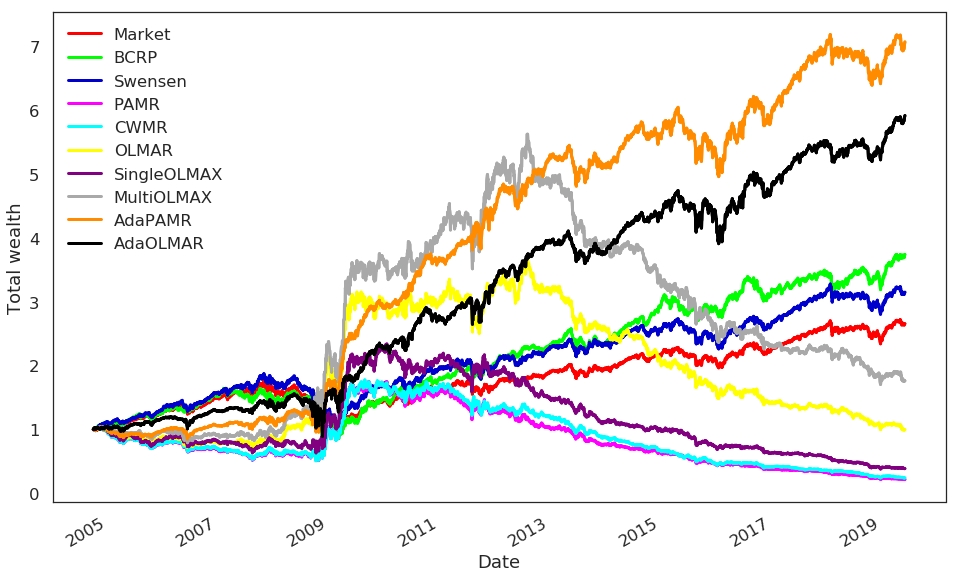
\includegraphics[width=\textwidth, height=\textheight, keepaspectratio]{etf-cumwealth-with-fees-and-adaAlgos}
%\caption{Cumulative wealth net of 0.1\% fees achieved by various strategies during the entire trading periods associated with the ETF data set (see Table~\ref{tab:etf-dataset}).}
%\label{fig:etf-cumwealth-with-adaAlgos}
%\end{figure}
%
%Table~\ref{tab:olps-metrics-etfs} reports the performance metrics of all the aforementioned algorithms on the ETF data set, in addition to the remaining ones enumerated in Section~\ref{sec:comparison-approaches}. As one would expect from Figure~\ref{fig:etf-cumwealth-with-adaAlgos}, AdaPAMR and AdaOLMAR dominate in terms of annual percentage yield. Furthermore, AdaPAMR is the least risky from a drawdown perspective, and exhibits the highest Sharpe ratio, AdaOLMAR having the third highest. The table also reveals that online Newton step (ONS) is a very competitive strategy in this setting, being the second best in terms of maximum drawdown risk and Sharpe ratio.
%
%\begin{table}
%  \caption{Performance metrics achieved by various OLPS algorithms on the ETF data set from Table~\ref{tab:etf-dataset}, subject to transaction fees of 0.1\%. The top two results are highlighted in \textbf{bold}.}
%  \label{tab:olps-metrics-etfs}
%  \centering
%  \resizebox{\textwidth}{!}{\begin{tabular}{lcccc}
%      \toprule
%      Algorithm & APY (\%) & Volatility Risk (\%) & MDD Risk (\%) & Sharpe Ratio \\
%      \midrule
%Market	& 6.87 & 14.90 & 45.33 & 0.45 \\
%Best stock & 8.83 & 18.47 & 55.45 & 0.46 \\
%BCRP & 9.39	& 18.81 & 47.97 & 0.48 \\
%Swensen	& 8.12 & 17.33 & 47.31 & 0.45 \\
%\\
%UP & 7.74 & \textbf{14.61} & 42.04 & 0.51 \\
%EG & 7.83 & \textbf{14.61} & 41.72 & 0.52 \\
%ONS & 10.14 & 15.22 & \textbf{32.64} & \textbf{0.63} \\
%\\
%PAMR & -9.95 & 24.54 & 87.74 & -0.43 \\
%CWMR & -9.29 & 24.75 & 86.54 & -0.39 \\
%OLMAR & -0.04 & 24.87 & 73.10 & -0.00 \\
%\\
%SingleOLMAX	& -6.29 & 24.61 & 83.81 & -0.26 \\
%MultiOLMAX-S & 3.93	& 24.62 & 69.71 & 0.16 \\
%MultiOLMAX-E & 5.84	& 24.84 & 66.34 & 0.23 \\
%\\
%AdaPAMR	& \textbf{14.24} & 18.87 & \textbf{26.79} & \textbf{0.71} \\
%AdaOLMAR & \textbf{12.86} & 21.13 & 42.81 & 0.57 \\
%      \bottomrule
%  \end{tabular}}
%\end{table}
%
%We end this chapter by recommending AdaPAMR as a general-purpose online portfolio selection algorithm that offers transaction-cost robustness and versatility to handle different asset classes and market regimes thanks to its hyperparameter-free nature.


\subsection{Empirical evaluation}
\label{sec:adapamr-eval}

\begin{mccorrection}
We now turn to implement the AdaPAMR and AdaOLMAR algorithms on the ETFs mentioned in Table~\ref{tab:etf-dataset}. Figure~\ref{fig:etf-cumwealth-with-adaAlgos} illustrates their respective cumulative wealth net of a transaction fee of 0.1\%, along with those achieved by the three benchmarks (Market, BCRP and the Swensen portfolio) and the non-adaptive reversion strategies (CWMR, PAMR, OLMAR, SingleOLMAX and MultiOLMAX). Furthermore, in order to empirically motivate the benefits of our approach, we include analogous variants of AdaPAMR and AdaOLMAR in which the learning rate is fixed to a schedule of $1/\sqrt{t}$, as in \citep{zinkevich03}. Perhaps at the expense of an abuse of terminology, we named these `AdaPAMR with $1/\sqrt{t}$ annealing' and `AdaOLMAR  with $1/\sqrt{t}$ annealing', respectively.

In comparison to the benchmarks, both the AdaPAMR and AdaOLMAR methods would have realised big gains at the end of the subprime mortgage crisis and, unlike their non-adaptive counterparts, managed to maintain that positive momentum all along thereafter, especially AdaPAMR. This explains the large discrepancy between their respective terminal wealths and that of all the other strategies plotted in the chart. Additionally, we notice that the variants of AdaPAMR and AdaOLMAR with Zinkevich's learning-rate schedule of $1/\sqrt{t}$ barely beat the Swensen portfolio, making them unattractive choices.
\end{mccorrection}
\begin{figure}[H]
\centering
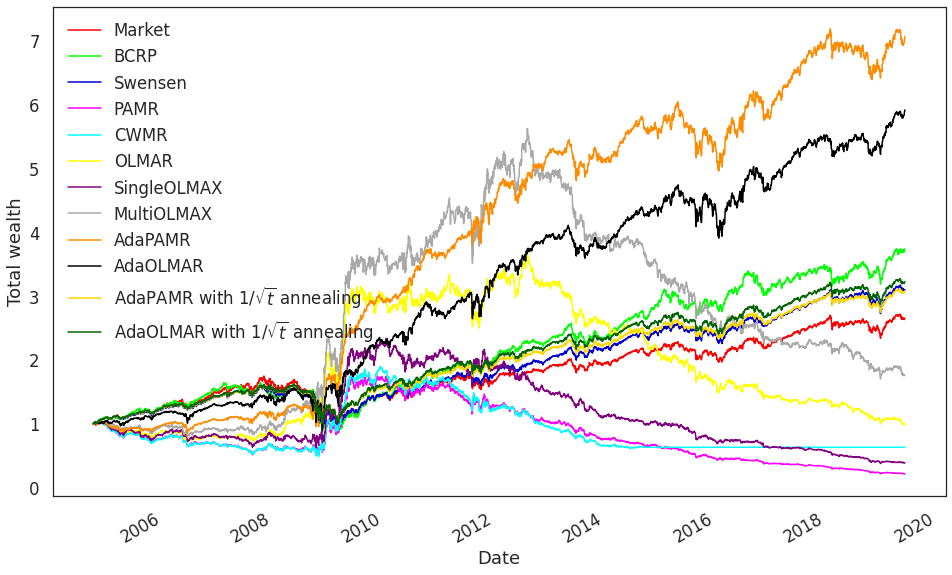
\includegraphics[width=\textwidth, height=\textheight, keepaspectratio]{etf-cumwealth-with-fees-and-adaAlgos-NEW}
\caption{Cumulative wealth net of 0.1\% fees achieved by various strategies during the entire trading periods associated with the ETF data set (see Table~\ref{tab:etf-dataset}).}
\label{fig:etf-cumwealth-with-adaAlgos}
\end{figure}

\begin{mccorrection}
Table~\ref{tab:olps-metrics-etfs} reports the performance metrics of all the aforementioned algorithms on the ETF data set, in addition to the remaining ones enumerated in Section~\ref{sec:comparison-approaches}. As one would expect from Figure~\ref{fig:etf-cumwealth-with-adaAlgos}, AdaPAMR and AdaOLMAR dominate in terms of annual percentage yield. Furthermore, AdaPAMR is the least risky from a drawdown perspective, and exhibits the highest Sharpe ratio.
\end{mccorrection}
\begin{table}
  \caption{Performance metrics achieved by various OLPS algorithms on the ETF data set from Table~\ref{tab:etf-dataset}, subject to transaction fees of 0.1\%. The top two results are highlighted in \textbf{bold}.}
  \label{tab:olps-metrics-etfs}
  \centering
  \resizebox{\textwidth}{!}{\begin{tabular}{lcccc}
      \toprule
      Algorithm & APY (\%) & Volatility Risk (\%) & MDD Risk (\%) & Sharpe Ratio \\
      \midrule
Market	& 6.87 & 14.90 & 45.33 & 0.45 \\
Best stock & 8.83 & 18.47 & 55.45 & 0.46 \\
BCRP & 9.39	& 18.81 & 47.97 & 0.48 \\
Swensen	& 8.12 & 17.33 & 47.31 & 0.45 \\
\\
UP & 7.74 & 14.61 & 42.04 & 0.51 \\
EG & 7.83 & 14.61 & 41.72 & 0.52 \\
ONS & 10.14 & 15.22 & \textbf{32.64} & 0.63 \\
\\
PAMR & -9.95 & 24.54 & 87.74 & -0.43 \\
CWMR & -9.29 & 24.75 & 86.54 & -0.39 \\
OLMAR & -0.04 & 24.87 & 73.10 & -0.00 \\
\\
SingleOLMAX	& -6.29 & 24.61 & 83.81 & -0.26 \\
MultiOLMAX-S & 3.93	& 24.62 & 69.71 & 0.16 \\
MultiOLMAX-E & 5.84	& 24.84 & 66.34 & 0.23 \\
\\
AdaPAMR with $1/\sqrt{t}$ annealing	& 8.50 & \textbf{12.95} & 37.07 & \textbf{0.66} \\
AdaOLMAR with $1/\sqrt{t}$ annealing	& 8.93 &	 \textbf{13.79} & 38.16 & 0.65 \\
AdaPAMR	& \textbf{14.24} & 18.87 & \textbf{26.79} & \textbf{0.71} \\
AdaOLMAR & \textbf{12.86} & 21.13 & 42.81 & 0.57 \\
      \bottomrule
  \end{tabular}}
\end{table}

We end this chapter by recommending AdaPAMR as a general-purpose online portfolio selection algorithm that offers transaction-cost robustness and versatility to handle different asset classes and market regimes thanks to its hyperparameter-free nature.